\section{Componenti}
\subsection{Introduzione}
 Partendo da quanto descritto nel documento di \textit{Specifica Tecnica}, è stato fatto uno studio approfondito delle tecnologie da utilizzare, in modo da poter scendere ad un livello di dettaglio tale da permettere di definire con chiarezza e precisione (seppure mantenendo la sintassi UML) la codifica dell'applicazione da parte dei programmatori.\\
 Questo si nota ed esempio all'interno del \textit{ViewPkg}: l'utilizzo di React, ha permesso:
 \begin{itemize}
	\item buon riutilizzo di codice, consentendo di ridurre fortemente il numero di componenti presentazionali che erano state progettate ad alto livello;
	\item semplificazione della procedura di costruzione dell'interfaccia grafica, grazie al principio di React "lifting state up", che consente la strutturazione dell'interfaccia in maniera fortemente modulare dal punto di vista puramente presentazionale, ma centralizzata dal punto di vista delle informazioni.
\end{itemize}
% v: 17
\subsection{DeGeOP}
\label{pkg::DeGeOP}
\begin{figure}[H]
	\centering
	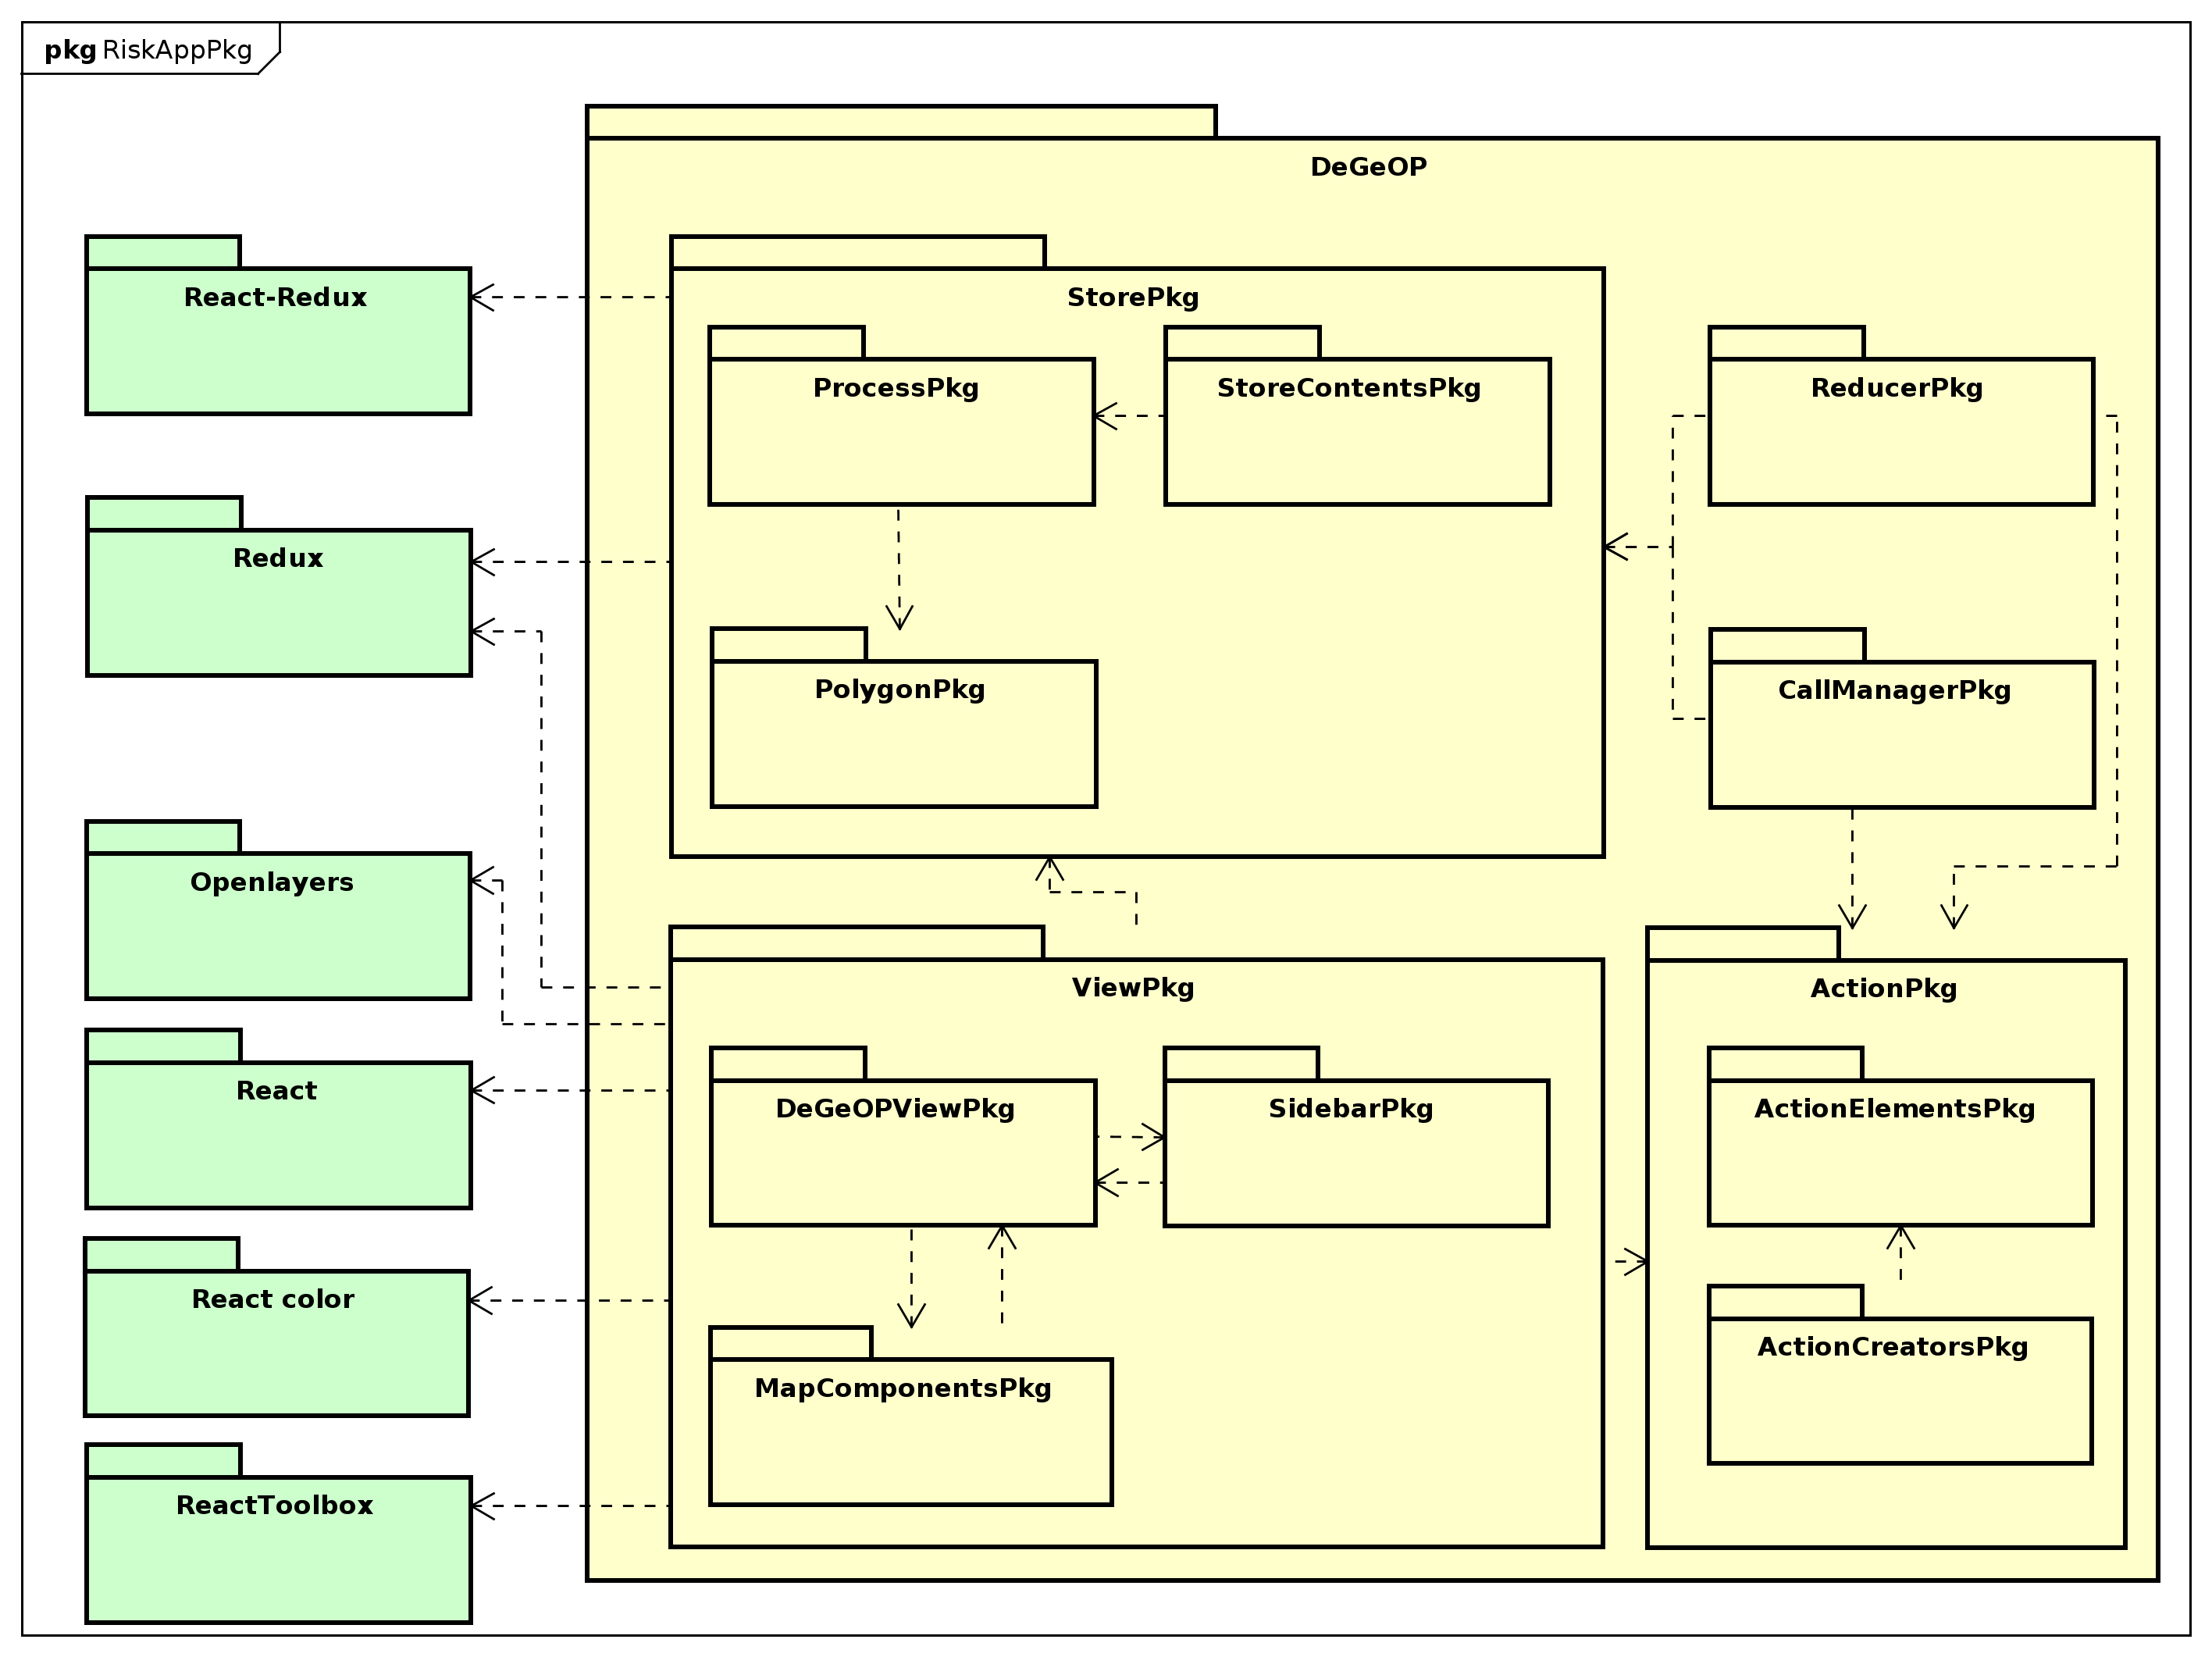
\includegraphics[width=\textwidth]{img/PkgDiagram/DeGeOPPkg.png}
	\caption{Schema componente DeGeOP}
\end{figure}
\subsubsection{Informazioni sul package}
\begin{itemize}
	\item \textbf{descrizione:} racchiude tutte le componenti necessarie per il front-end del prodotto;
	\item \textbf{package contenuti:}
	\begin{itemize}
		\item DeGeOP::\hyperref[pkg::ActionPkg]{ActionPkg};
		\item DeGeOP::\hyperref[pkg::CallManagerPkg]{CallManagerPkg};
		\item DeGeOP::\hyperref[pkg::ReducerPkg]{ReducerPkg};
		\item DeGeOP::\hyperref[pkg::StorePkg]{StorePkg};
		\item DeGeOP::\hyperref[pkg::ViewPkg]{ViewPkg}.
	\end{itemize}
\end{itemize}
\newpage
\subsection{DeGeOP::StorePkg}
\label{pkg::StorePkg}
\begin{figure}[H]
	\centering
	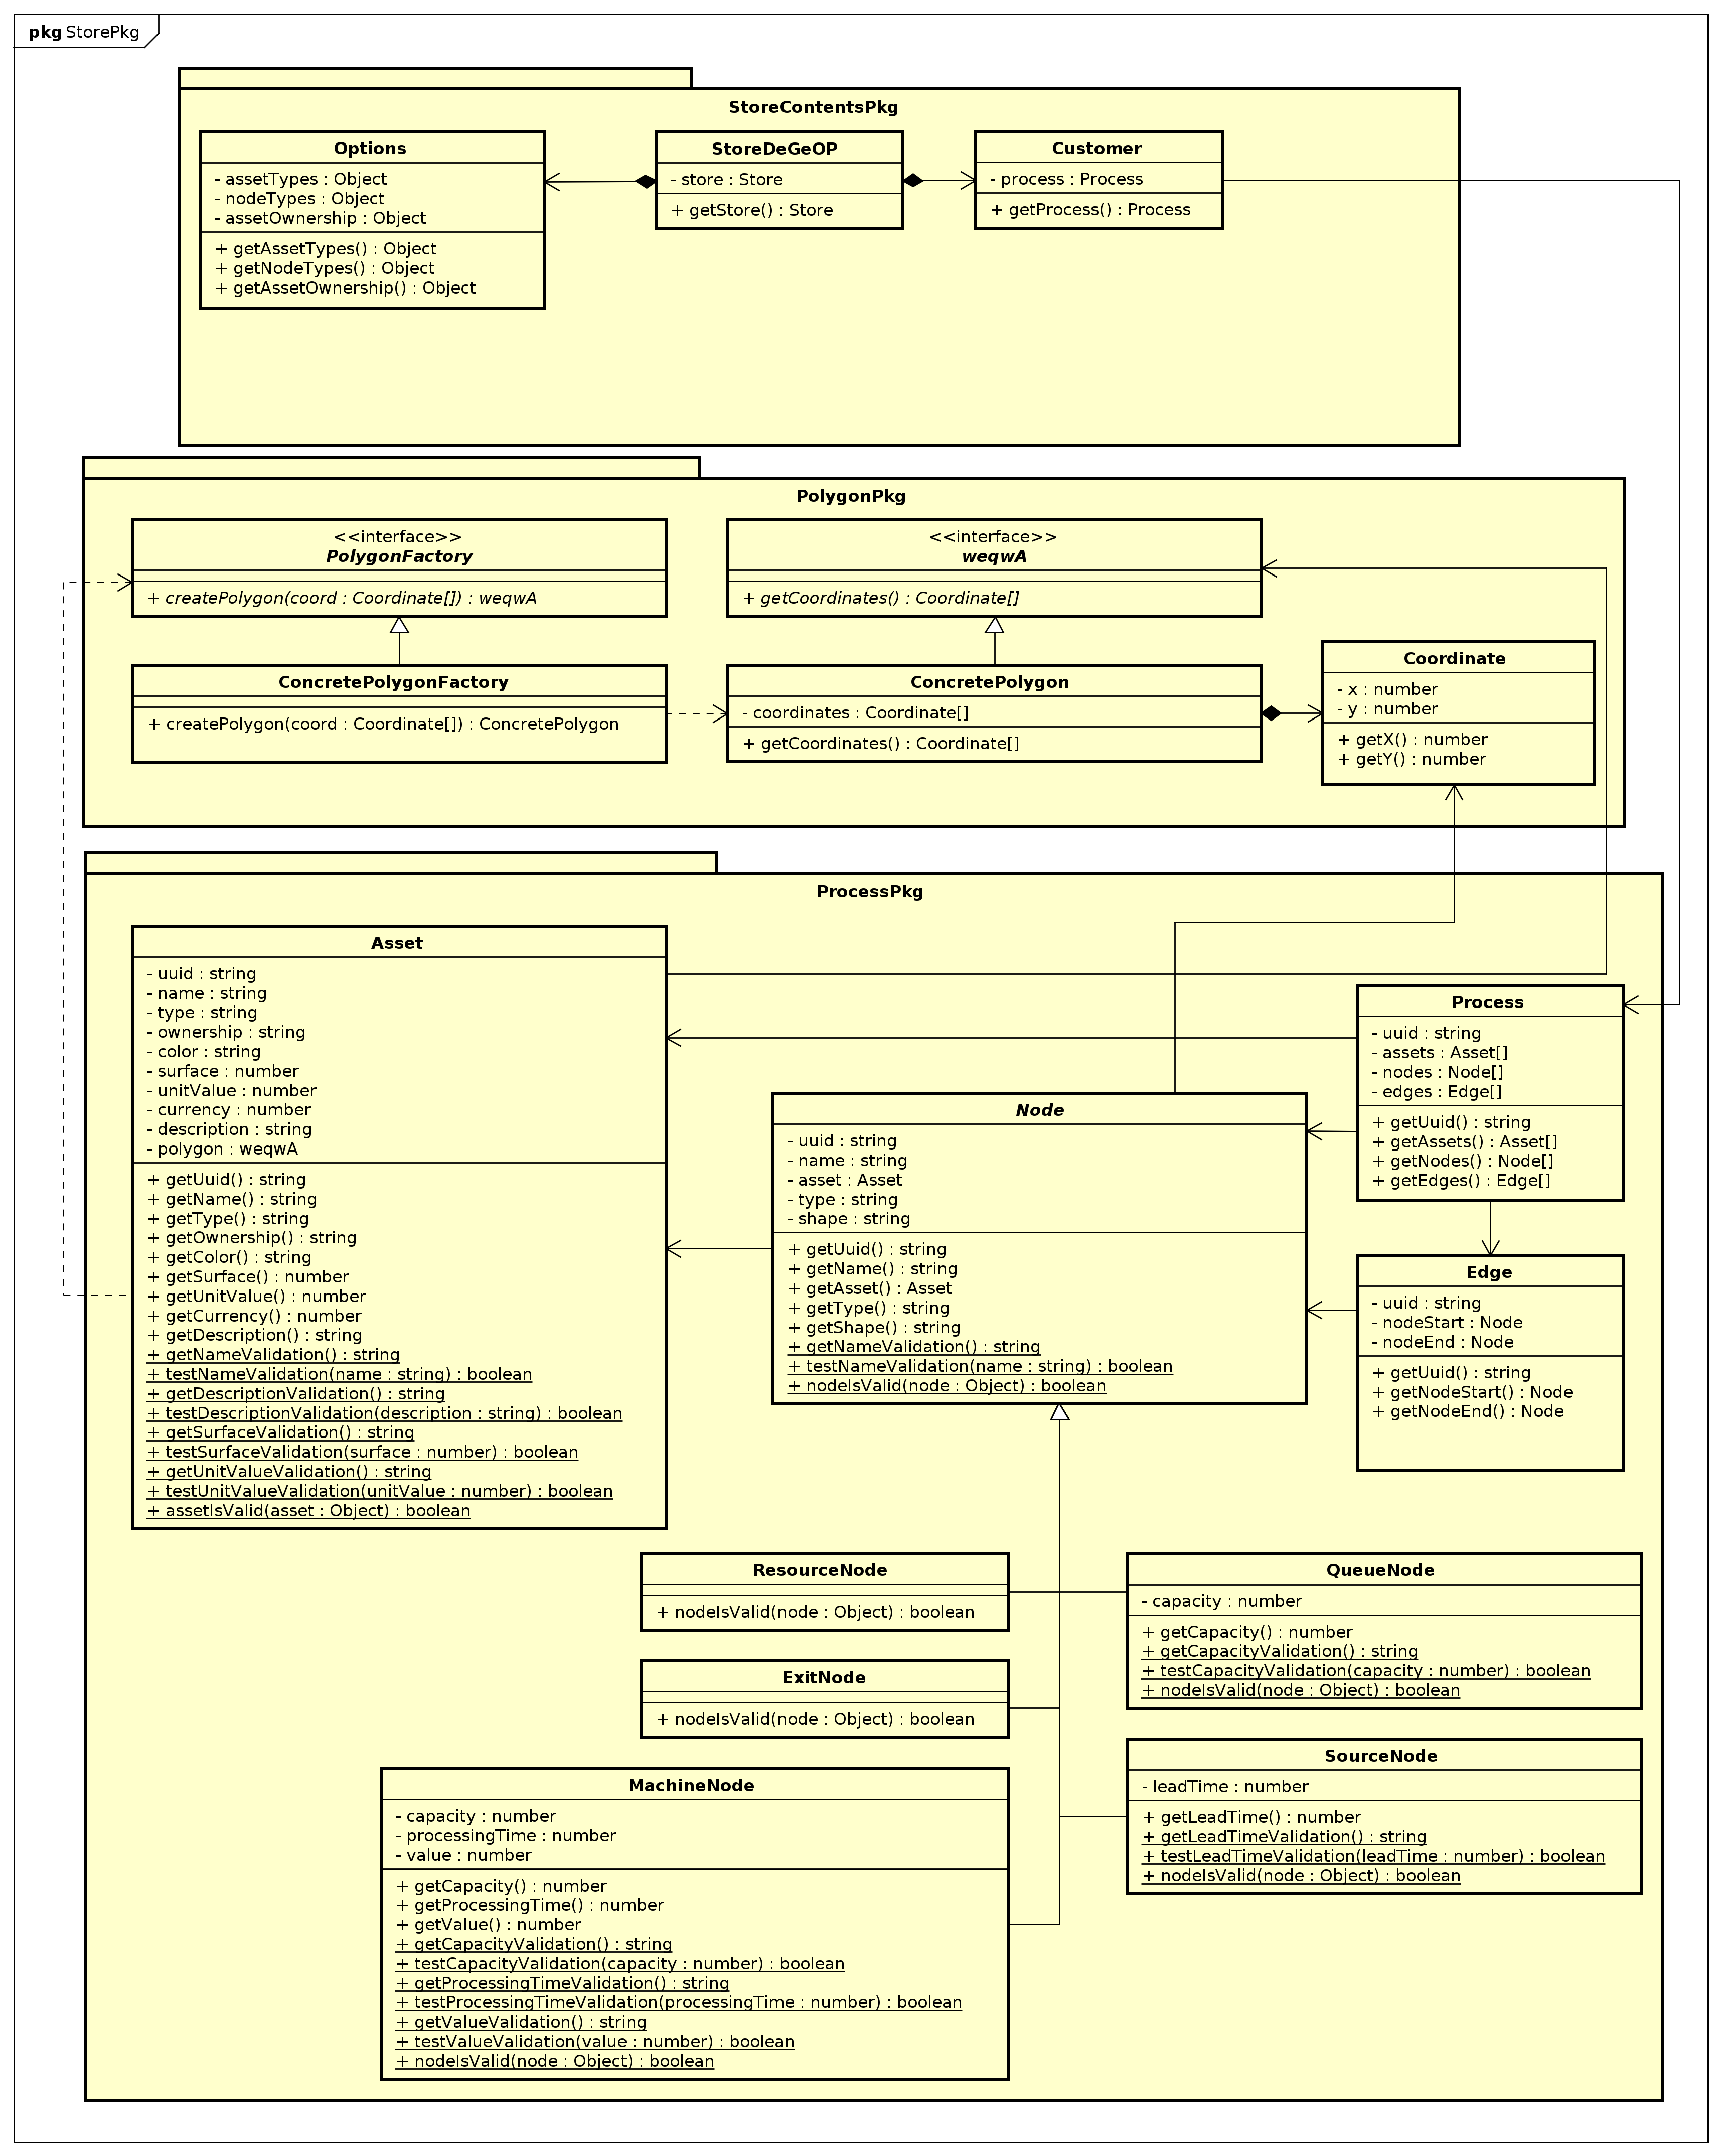
\includegraphics[width=\textwidth]{img/PkgDiagram/StorePkg.png}
	\caption{Schema componente DeGeOP::StorePkg}
\end{figure}
\subsubsection{Informazioni sul package}
\begin{itemize}
	\item \textbf{descrizione:} racchiude le componenti utilizzate per la memorizzazione e rappresentazione dei dati;
	\item \textbf{padre:} \hyperref[pkg::DeGeOP]{DeGeOP};
	\item \textbf{package contenuti:}
	\begin{itemize}
		\item StorePkg::\hyperref[pkg::PolygonPkg]{PolygonPkg};
		\item StorePkg::\hyperref[pkg::ProcessPkg]{ProcessPkg};
		\item StorePkg::\hyperref[pkg::StoreContentsPkg]{StoreContentsPkg}.
	\end{itemize}
	\item \textbf{interazioni con altri package:} 
	\begin{itemize}
		\item IN CallManagerPkg: subscribe sullo store;
		\item IN ReducerPkg: applicazione di cambiamenti di stato;
		\item IN ViewPkg: subscribe sullo store;
		\item OUT React-Redux: utilizzo di Provider per evitare di passare lo store come proprietà alle componenti React;
		\item OUT Redux: creazione Store utilizzando il metodo createStore().
	\end{itemize}
\end{itemize}
\newpage
\subsection{DeGeOP::StorePkg::StoreContentsPkg}
\label{pkg::StoreContentsPkg}
\subsubsection{Informazioni sul package}
\begin{itemize}
	\item \textbf{descrizione:} racchiude le componenti che implementano il concetto di store dell'architettura Redux;
	\item \textbf{padre:} \hyperref[pkg::StorePkg]{StorePkg};
	\item \textbf{interazioni con altri package:} 
	\begin{itemize}
		\item OUT AnalysisPkg: riferimento ad analisi di danno;
		\item OUT ProcessPkg: riferimento a processo;
		\item OUT React-Redux: utilizzo del Provider;
		\item OUT Redux: creazione store.
	\end{itemize}
	\item \textbf{classi contenute:}
	\begin{itemize}
		\item Customer;
		\item Options;
		\item StoreDeGeOP.
	\end{itemize}
\end{itemize}
\subsubsection{Classi}
\paragraph{Customer}
\begin{itemize}
	\begin{figure}[H]
		\centering
		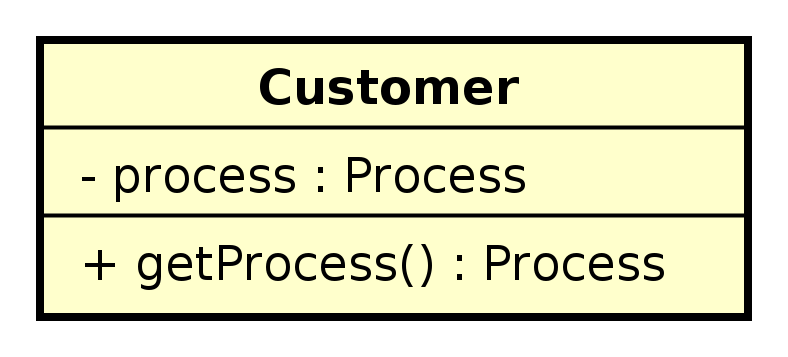
\includegraphics[width=0.3\textwidth]{./img/Customer.png}
		\caption{Diagramma classe Customer}
	\end{figure}
	\item \textbf{descrizione:} rappresenta l'assicurando;
	\item \textbf{utilizzo:} viene utilizzato nello Store per memorizzare l'assicurando;
	\item \textbf{attributi:}
	\begin{itemize}
		\item -process : Process\begin{itemize}
			\item rappresenta il processo produttivo dell'assicurando.\end{itemize}
	\end{itemize}
	\item \textbf{metodi:}
	\begin{itemize}
		\item +getProcess() : Process\newline
		il metodo restituisce il processo produttivo dell'assicurando
	\end{itemize}
\end{itemize}
\paragraph{Options}
\begin{itemize}
	\begin{figure}[H]
		\centering
		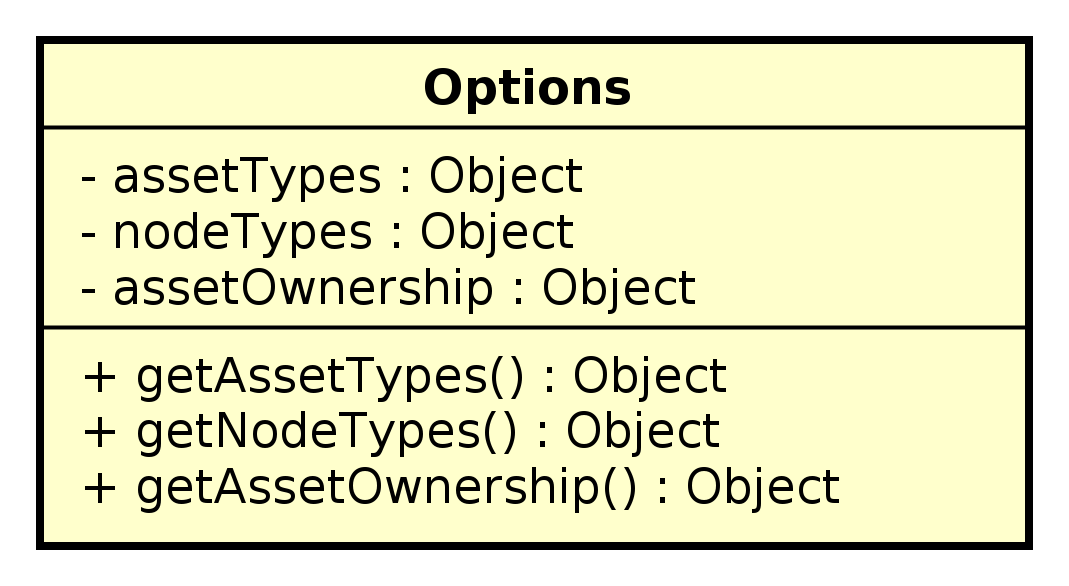
\includegraphics[width=0.3\textwidth]{./img/Options.png}
		\caption{Diagramma classe Options}
	\end{figure}
	\item \textbf{descrizione:} classe contenente le associazioni tra codice e valore dei campi dati degli altri elementi dello store;
	\item \textbf{utilizzo:} viene utilizzata per associare codice e valore dei campi dati degli altri elementi dello store;
	\item \textbf{attributi:}
	\begin{itemize}
		\item -assetOwnership : Object\begin{itemize}
			\item associazione chiave valore delle tipologie di soggetti di appartenenza dell'asset.\end{itemize}
		\item -assetTypes : Object\begin{itemize}
			\item associazione chiave valore delle tipologie di materiale dell'asset.\end{itemize}
		\item -nodeTypes : Object\begin{itemize}
			\item associazione chiave valore delle tipologie di materiale del nodo.\end{itemize}
	\end{itemize}
	\item \textbf{metodi:}
	\begin{itemize}
		\item +getAssetOwnership() : Object\newline
		il metodo ritorna l'oggetto assetOwnership
		\item +getAssetTypes() : Object\newline
		il metodo ritorna l'oggetto assetTypes
		\item +getNodeTypes() : Object\newline
		il metodo ritorna l'oggetto nodeTypes
	\end{itemize}
	\item \textbf{relazioni con altre classi:} 
	\begin{itemize}
		\item IN OptionReducer;
		\item IN StoreDeGeOP.
	\end{itemize}
\end{itemize}
\paragraph{StoreDeGeOP}
\begin{itemize}
	\begin{figure}[H]
		\centering
		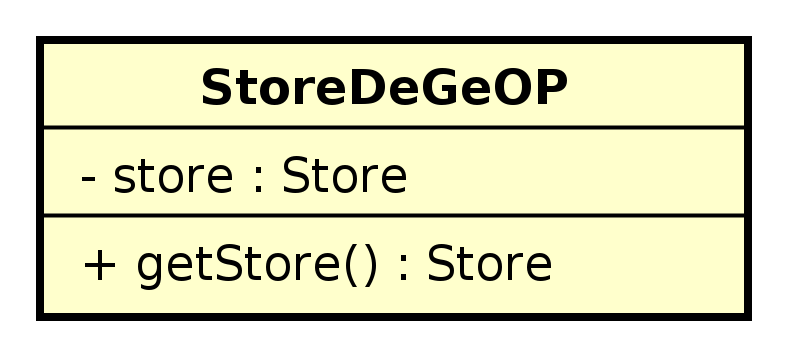
\includegraphics[width=0.3\textwidth]{./img/StoreDeGeOP.png}
		\caption{Diagramma classe StoreDeGeOP}
	\end{figure}
	\item \textbf{descrizione:} rappresenta una classe che incapsula uno Store creato utilizzando Redux;
	\item \textbf{utilizzo:} viene utilizzato per memorizzare lo stato dell'applicazione.
	Le componenti che effettuano il subscribe sullo Store verranno notificate ad ogni cambiamento di stato dello Store;
	\item \textbf{attributi:}
	\begin{itemize}
		\item -customer : Customer\begin{itemize}
			\item rappresenta il cliente che gestiamo.\end{itemize}
		\item -store : Object\begin{itemize}
			\item rappresenta l'oggetto Store creato utilizzando Redux.\end{itemize}
	\end{itemize}
	\item \textbf{metodi:}
	\begin{itemize}
		\item +getStore() : Object\newline
		il metodo restituisce lo store creato utilizzando Redux
	\end{itemize}
	\item \textbf{relazioni con altre classi:} 
	\begin{itemize}
		\item IN Reducer;
		\item OUT Options.
	\end{itemize}
\end{itemize}
\newpage
\subsection{DeGeOP::StorePkg::ProcessPkg}
\label{pkg::ProcessPkg}
\subsubsection{Informazioni sul package}
\begin{itemize}
	\item \textbf{descrizione:} racchiude le componenti necessarie alla rappresentazione del processo produttivo dell'assicurando;
	\item \textbf{padre:} \hyperref[pkg::StorePkg]{StorePkg};
	\item \textbf{interazioni con altri package:} 
	\begin{itemize}
		\item IN StoreContentsPkg: riferimento a processo;
		\item OUT PolygonPkg: riferimento ad un poligono.
	\end{itemize}
	\item \textbf{classi contenute:}
	\begin{itemize}
		\item Asset;
		\item Edge;
		\item ExitNode;
		\item MachineNode;
		\item Node;
		\item Process;
		\item QueueNode;
		\item ResourceNode;
		\item SourceNode.
	\end{itemize}
\end{itemize}
\subsubsection{Classi}
\paragraph{Asset}
\begin{itemize}
	\begin{figure}[H]
		\centering
		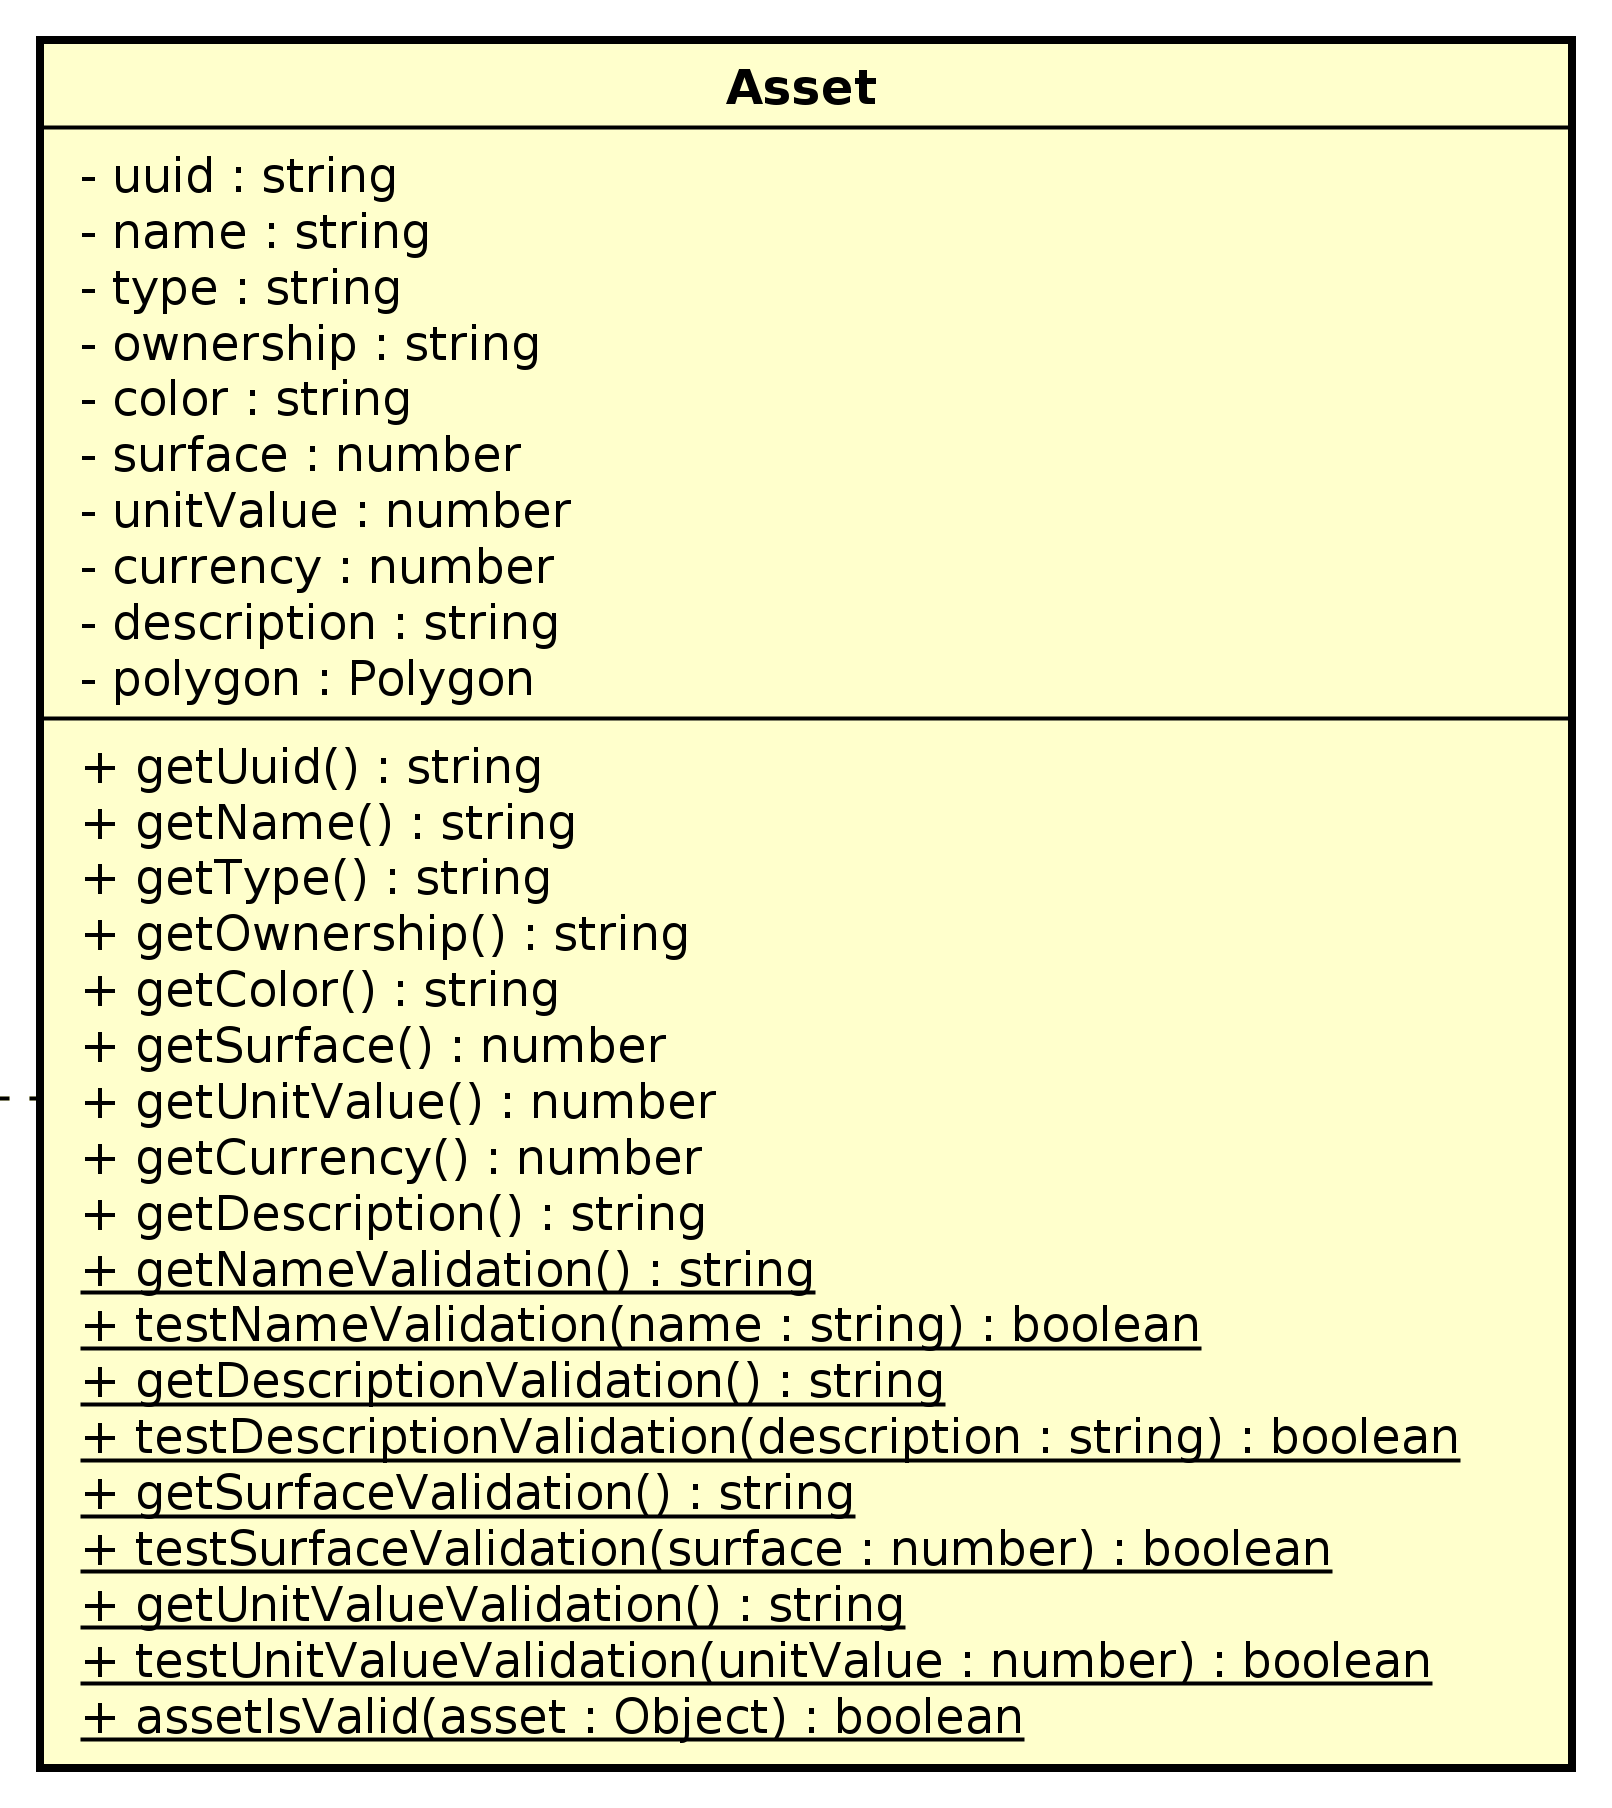
\includegraphics[width=0.3\textwidth]{./img/Asset.png}
		\caption{Diagramma classe Asset}
	\end{figure}
	\item \textbf{descrizione:} rappresenta un fabbricato di interesse per il processo produttivo dell'assicurando;
	\item \textbf{utilizzo:} sono contenuti all'interno di Process;
	\item \textbf{attributi:}
	\begin{itemize}
		\item -color : string\begin{itemize}
			\item indica il colore dell'asset.\end{itemize}
		\item -currency : number\begin{itemize}
			\item indica la valuta utilizzata.\end{itemize}
		\item -description : string\begin{itemize}
			\item rappresenta la descrizione dell'asset.\end{itemize}
		\item -name : string\begin{itemize}
			\item rappresenta il nome dell'asset.\end{itemize}
		\item -ownership : string\begin{itemize}
			\item rappresenta l'appartenenza dell'asset.\end{itemize}
		\item -surface : number\begin{itemize}
			\item rappresenta la dimensione, in mq, dell'asset.\end{itemize}
		\item -type : string\begin{itemize}
			\item rappresenta la tipologia dell'asset.\end{itemize}
		\item -unitValue : string\begin{itemize}
			\item indica il valore economico dell'asset.\end{itemize}
		\item -uuid : string\begin{itemize}
			\item rappresenta l'identificativo dell'asset (uuid).\end{itemize}
	\end{itemize}
	\item \textbf{metodi:}
	\begin{itemize}
		\item +assetIsValid(asset) : boolean\newline
		il metodo testa che i parametri con cui l'asset sta per essere creato siano validi
		\begin{itemize}
			\item asset : Object\\
			oggetto contenente i parametri di un Asset che dovrà essere validato.
		\end{itemize}
		\item +getColor() : string\newline
		il metodo ritorna il colore dell'asset
		\item +getCurrency() : number\newline
		il metodo ritorna la valuta utilizzata per l'asset
		\item +getDescription() : string\newline
		il metodo ritorna la descrizione dell'asset
		\item +getDescriptionValidation() : string\newline
		il metodo ritorna l'espressione regolare che indica una stringa non contenente le seguenti caratteristiche: vuota; più lunga di 5000 caratteri; inizia e/o finisce con uno spazio; contiene caratteri speciali
		diversi dall’apostrofo
		\item +getName() : string\newline
		ritorna il nome dell'asset
		\item +getNameValidation() : string\newline
		il metodo ritorna l'espressione regolare che indica una stringa non contenente le seguenti caratteristiche: più lunga di 50 caratteri; inizia e/o finisce con uno spazio; contiene caratteri speciali.
		\item +getOwnership() : string\newline
		il metodo ritorna l'appartenenza dell'asset
		\item +getSurface() : number\newline
		il metodo ritorna la dimensione dell'asset
		\item +getSurfaceValidation() : string\newline
		il metodo ritorna l'espressione regolare che indica una stringa non contenente le seguenti caratteristiche:vuota; più lunga di 5 cifre per la parte intera; più di 2 per la parte decimale;
		
		\item +getType() : string\newline
		il metodo ritorna la tipologia dell'asset
		\item +getUnitValue() : string\newline
		il metodo ritorna il valore economico dell'asset
		\item +getUnitValueValidation() : string\newline
		il metodo ritorna l'espressione regolare che indica una stringa non contenente le seguenti caratteristiche: vuota; più lunga di 5 cifre per la parte intera; più di 2 per la parte decimale
		\item +getUuid() : string\newline
		il metodo ritorna l'uuid dell'asset
		\item +testDescriptionValidation(description) : boolean\newline
		il metodo ritorna true solamente se il valore ricevuto in input, come parametro, è ritenuto valido.
		\begin{itemize}
			\item description : string\\
			rappresenta la descrizione dell'asset.
		\end{itemize}
		\item +testNameValidation(name) : boolean\newline
		il metodo ritorna true solamente se il valore ricevuto in input, come parametro, è ritenuto valido.
		\begin{itemize}
			\item name : string\\
			rappresenta il nome dell'asset.
		\end{itemize}
		\item +testSurfaceValidation(surface) : boolean\newline
		il metodo ritorna true solamente se il valore ricevuto in input, come parametro, è ritenuto valido.
		\begin{itemize}
			\item surface : number\\
			rappresenta la dimensione, in mq, dell'asset.
		\end{itemize}
		\item +testUnitValueValidation(unitValue) : boolean\newline
		il metodo ritorna true solamente se il valore ricevuto in input, come parametro, è ritenuto valido.
		\begin{itemize}
			\item unitValue : number\\
			indica il valore economico dell'asset.
		\end{itemize}
	\end{itemize}
	\item \textbf{relazioni con altre classi:} 
	\begin{itemize}
		\item IN AssetReducer.
	\end{itemize}
\end{itemize}
\paragraph{Edge}
\begin{itemize}
	\begin{figure}[H]
		\centering
		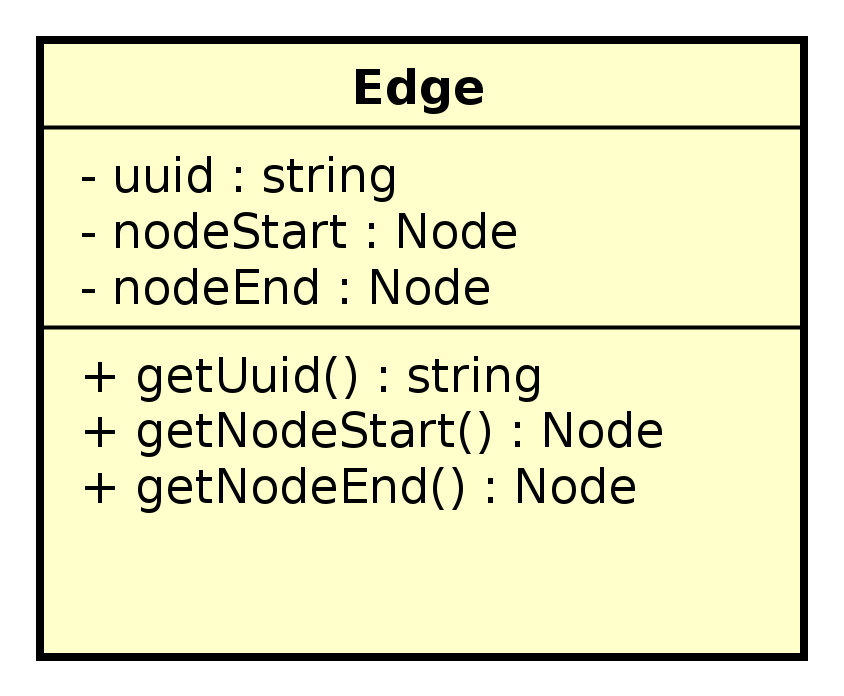
\includegraphics[width=0.3\textwidth]{./img/Edge.png}
		\caption{Diagramma classe Edge}
	\end{figure}
	\item \textbf{descrizione:} rappresenta un arco che collega due nodi tra di loro; un arco indica che i nodi sono in correlazione tra di loro;
	\item \textbf{utilizzo:} è contenuto all'interno di Process;
	\item \textbf{attributi:}
	\begin{itemize}
		\item -nodeEnd : Node\begin{itemize}
			\item rappresenta il nodo di arrivo.\end{itemize}
		\item -nodeStart : Node\begin{itemize}
			\item rappresenta il nodo di partenza.\end{itemize}
		\item -uuid : string\begin{itemize}
			\item rappresenta il codice identificativo dell'arco (uuid).\end{itemize}
	\end{itemize}
	\item \textbf{metodi:}
	\begin{itemize}
		\item +getNodeEnd() : Node\newline
		il metodo restituisce il nodo di arrivo
		\item +getNodeStart() : Node\newline
		il metodo restituisce il nodo di partenza
		\item +getUuid() : string\newline
		il metodo restituisce il codice identificativo dell'arco (uuid)
	\end{itemize}
	\item \textbf{relazioni con altre classi:} 
	\begin{itemize}
		\item IN EdgeReducer.
	\end{itemize}
\end{itemize}
\paragraph{ExitNode}
\begin{itemize}
	\begin{figure}[H]
		\centering
		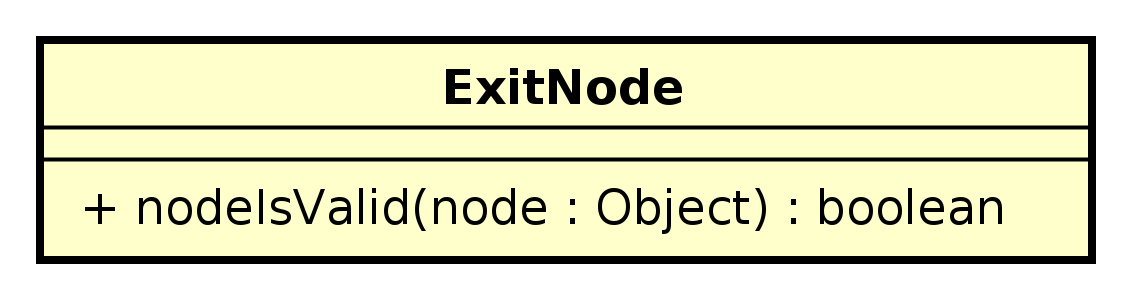
\includegraphics[width=0.3\textwidth]{./img/ExitNode.png}
		\caption{Diagramma classe ExitNode}
	\end{figure}
	\item \textbf{descrizione:} rappresenta un nodo di tipo Uscita;
	\item \textbf{utilizzo:} è contenuto all'interno di Process;
	\item \textbf{metodi:}
	\begin{itemize}
		\item +nodeIsValid() : boolean\newline
		il metodo testa che i parametri con cui il nodo sta per essere creato siano validi
	\end{itemize}
\end{itemize}
\paragraph{MachineNode}
\begin{itemize}
	\begin{figure}[H]
		\centering
		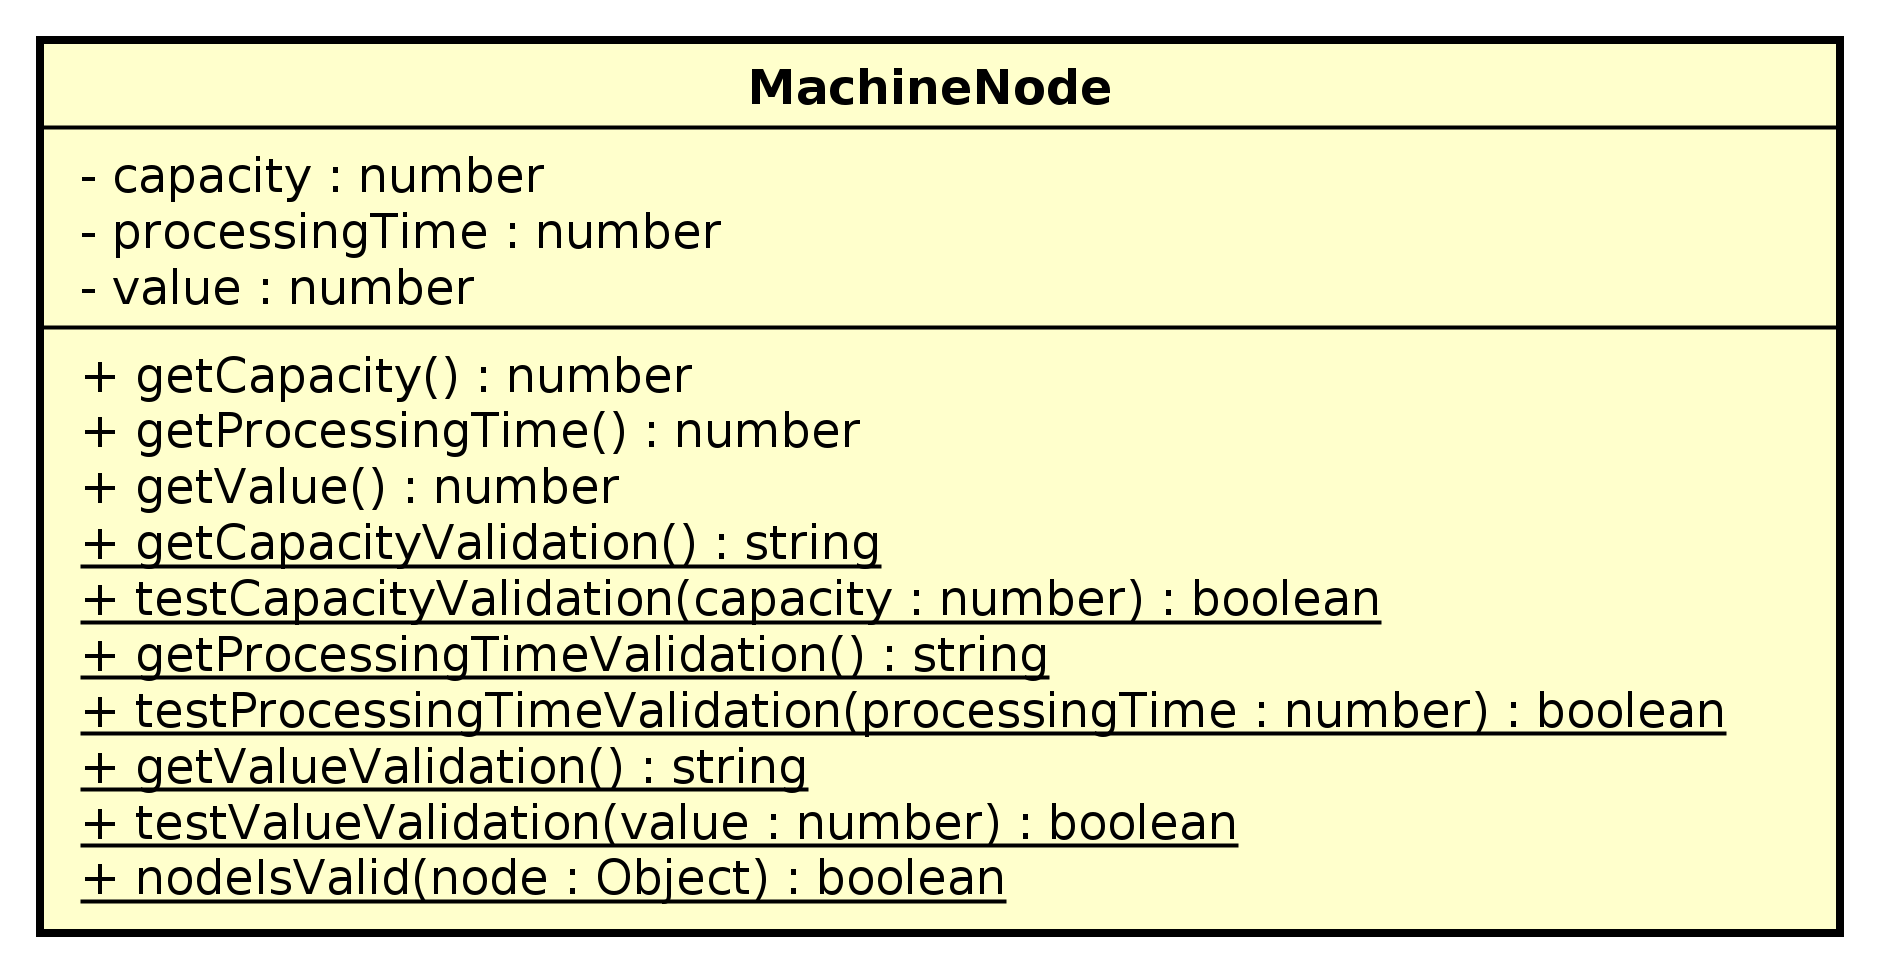
\includegraphics[width=0.3\textwidth]{./img/MachineNode.png}
		\caption{Diagramma classe MachineNode}
	\end{figure}
	\item \textbf{descrizione:} rappresenta un nodo di tipo Macchina;
	\item \textbf{utilizzo:} è contenuto all'interno di Process;
	\item \textbf{attributi:}
	\begin{itemize}
		\item -capacity : number\begin{itemize}
			\item rappresenta la capacità del nodo.\end{itemize}
		\item -processingTime : number\begin{itemize}
			\item rappresenta il tempo di processo del nodo.\end{itemize}
		\item -value : number\begin{itemize}
			\item rappresenta il valore del nodo.\end{itemize}
	\end{itemize}
	\item \textbf{metodi:}
	\begin{itemize}
		\item +getCapacity() : number\newline
		il metodo ritorna la capacità del nodo
		\item +getCapacityValidation() : string\newline
		il metodo ritorna l'espressione regolare che indica una stringa non contenente le seguenti caratteristiche: vuota; più lunga di 5 cifre per la parte intera; più di 2 per la parte decimale;
		\item +getProcessingTime() : number\newline
		il metodo ritorna il tempo di processo del nodo
		\item +getProcessingTimeValidation() : string\newline
		il metodo ritorna l'espressione regolare che indica una stringa non contenente le seguenti caratteristiche: vuota; più lunga di 5 cifre per la parte intera; più di 2 per la parte decimale;
		\item +getValue() : number\newline
		il metodo ritorna il valore del nodo
		\item +getValueValidation() : string\newline
		il metodo ritorna l'espressione regolare che indica una stringa non contenente le seguenti caratteristiche: vuota; più lunga di 20 cifre per la parte intera; più di 2 per la parte decimale
		\item +nodeIsValid(node) : boolean\newline
		il metodo testa se i parametri con cui il nodo sta per essere creato sono validi
		\begin{itemize}
			\item node : Object\\
			oggetto che rappresenta i parametri con cui il nodo sta per essere creato.
		\end{itemize}
		\item +testCapacityValidation() : boolean\newline
		il metodo testa se la capacità del nodo valida
		\item +testProcessingTimeValidation(processingTime) : boolean\newline
		il metodo testa se il tempo di processo valida
		\begin{itemize}
			\item processingTime : number\\
			rappresenta il tempo di processo del nodo.
		\end{itemize}
		\item +testValueValidation(value) : boolean\newline
		il metodo testa se il valore del nodo valida
		\begin{itemize}
			\item value : number\\
			rappresenta il valore del nodo.
		\end{itemize}
	\end{itemize}
\end{itemize}
\paragraph{Node}
\begin{itemize}
	\begin{figure}[H]
		\centering
		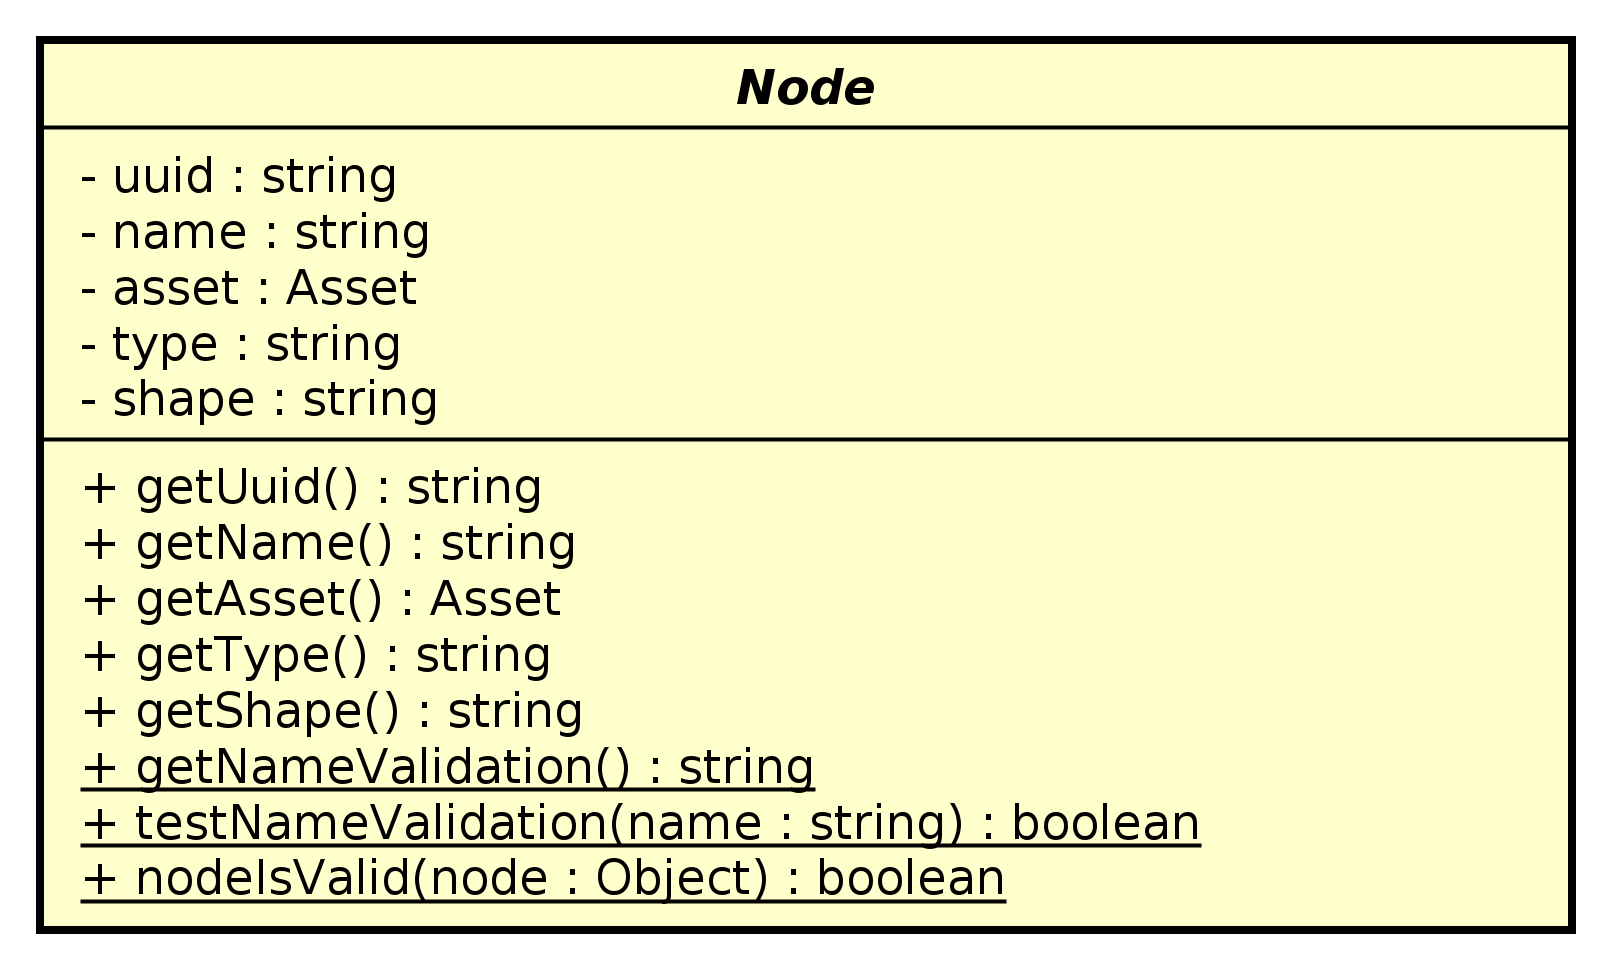
\includegraphics[width=0.3\textwidth]{./img/Node.png}
		\caption{Diagramma classe Node}
	\end{figure}
	\item \textbf{descrizione:} rappresenta un nodo contenuto all'interno di un Asset ;
	\item \textbf{utilizzo:} è contenuto all'interno di Process;
	\item \textbf{attributi:}
	\begin{itemize}
		\item -asset : Asset\begin{itemize}
			\item rappresenta l'asset a cui il nodo appartiene.\end{itemize}
		\item -name : string\begin{itemize}
			\item rappresenta il nome del nodo.\end{itemize}
		\item -shape : string\begin{itemize}
			\item rappresenta la forma del nodo.\end{itemize}
		\item -type : string\begin{itemize}
			\item rappresenta la classe del nodo.\end{itemize}
		\item -uuid : string\begin{itemize}
			\item rappresenta il codice identificativo del nodo (uuid).\end{itemize}
	\end{itemize}
	\item \textbf{metodi:}
	\begin{itemize}
		\item +getAsset() : Asset\newline
		il metodo ritorna l'asset di appartenenza del nodo
		\item +getName() : string\newline
		il metodo ritorna il codice identificativo del nodo
		\item +getNameValidation() : string\newline
		il metodo ritorna l'espressione regolare che indica una stringa non contenente le seguenti caratteristiche: vuota; più
		lunga di 50 caratteri; inizia e/o finisce con uno spazio; contiene caratteri speciali;
		\item +getShape() : string\newline
		il metodo ritorna la forma del nodo
		\item +getType() : string\newline
		il metodo ritorna la classe del nodo
		\item +getUuid() : string\newline
		il metodo ritorna il codice identificativo del nodo (uuid)
		\item +nodeIsValid() : boolean\newline
		il metodo testa che i parametri con cui il nodo sta per essere creato siano validi
		\item +testNameValidation(name) : boolean\newline
		il metodo ritorna true solamente se il valore ricevuto in input, come parametro, è ritenuto valido.
		\begin{itemize}
			\item name : string\\
			rappresenta il nome del nodo.
		\end{itemize}
	\end{itemize}
	\item \textbf{relazioni con altre classi:} 
	\begin{itemize}
		\item IN NodeReducer.
	\end{itemize}
\end{itemize}
\paragraph{Process}
\begin{itemize}
	\begin{figure}[H]
		\centering
		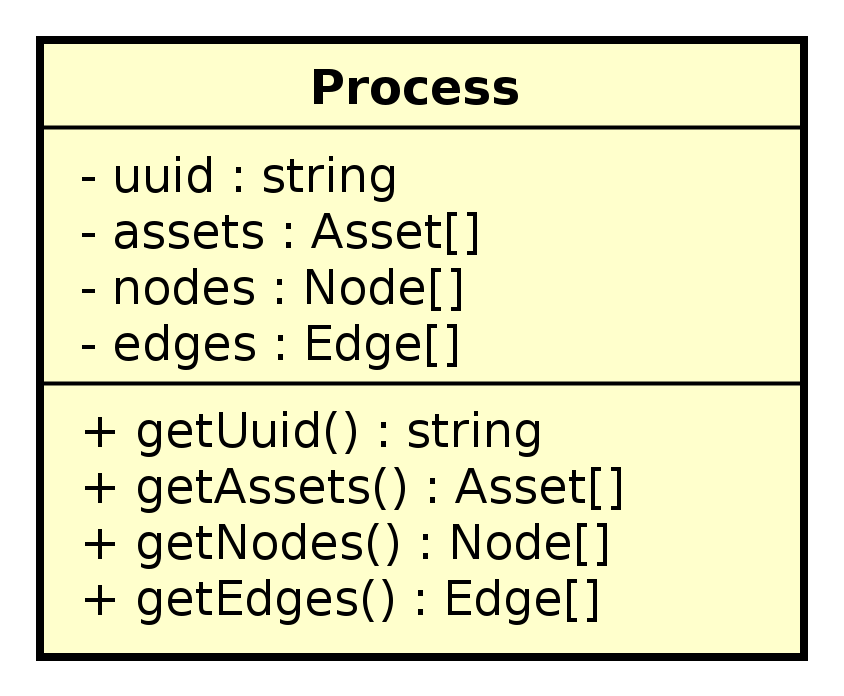
\includegraphics[width=0.3\textwidth]{./img/Process.png}
		\caption{Diagramma classe Process}
	\end{figure}
	\item \textbf{descrizione:} rappresenta un processo produttivo dell'azienda dell'assicurando;
	\item \textbf{utilizzo:} è memorizzato nello Store;
	\item \textbf{attributi:}
	\begin{itemize}
		\item -assets : Asset[ ]\begin{itemize}
			\item rappresenta gli asset facenti parti del processo produttivo.\end{itemize}
		\item -edges : Edge [ ]\begin{itemize}
			\item rappresenta gli archi che effettuano i collegamenti nel processo produttivo.\end{itemize}
		\item -nodes : Node [ ]\begin{itemize}
			\item rappresenta i nodi facenti parti del processo produttivo.\end{itemize}
		\item -uuid : string\begin{itemize}
			\item rappresenta l'identificativo del processo (uuid).\end{itemize}
	\end{itemize}
	\item \textbf{metodi:}
	\begin{itemize}
		\item +getAssets() : Asset[ ]\newline
		il metodo ritorna gli asset facenti parti del processo produttivo
		\item +getEdges() : Edge [ ]\newline
		il metodo ritorna gli archi che effettuano i collegamenti nel processo produttivo
		\item +getNodes() : Node [ ]\newline
		il metodo ritorna i nodi facenti parti del processo produttivo
		\item +getUuid() : string\newline
		il metodo ritorna il codice identificativo (uuid) del processo
	\end{itemize}
\end{itemize}
\paragraph{QueueNode}
\begin{itemize}
	\begin{figure}[H]
		\centering
		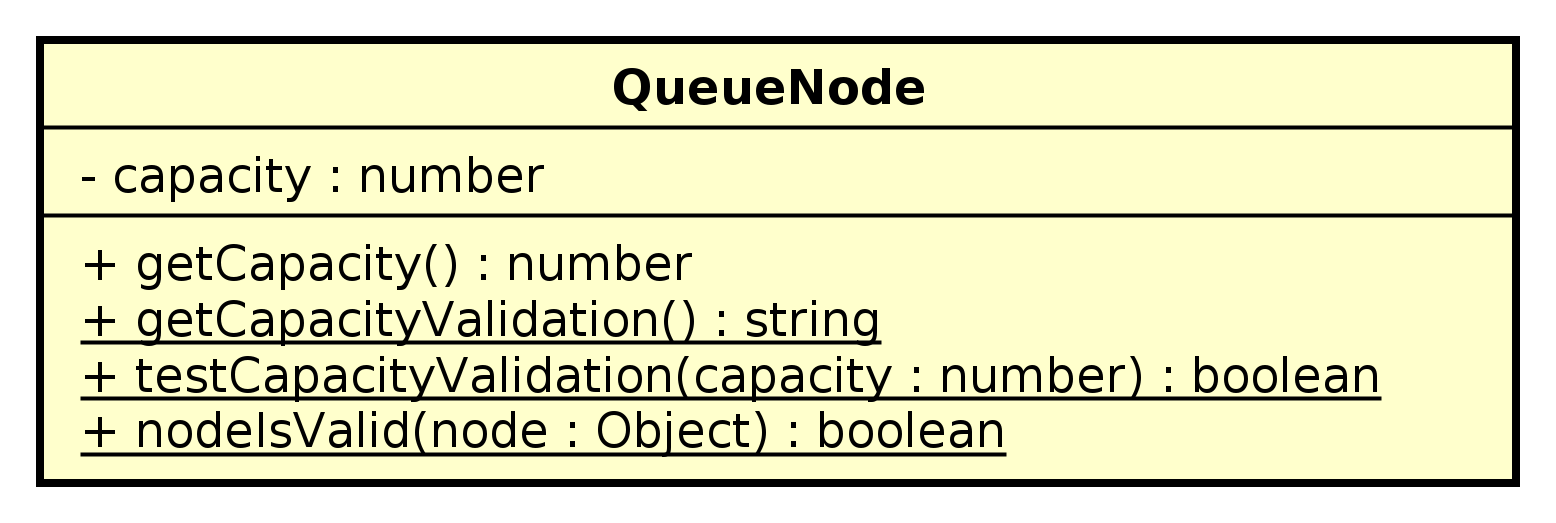
\includegraphics[width=0.3\textwidth]{./img/QueueNode.png}
		\caption{Diagramma classe QueueNode}
	\end{figure}
	\item \textbf{descrizione:} rappresenta un nodo di tipo Coda;
	\item \textbf{utilizzo:} è contenuto all'interno di Process;
	\item \textbf{attributi:}
	\begin{itemize}
		\item -capacity : number\begin{itemize}
			\item rappresenta la capacità del nodo coda.\end{itemize}
	\end{itemize}
	\item \textbf{metodi:}
	\begin{itemize}
		\item +getCapacity() : number\newline
		il metodo ritorna la capacità del nodo
		\item +getCapacityValidation() : string\newline
		il metodo ritorna l'espressione regolare che indica una stringa non contenente le seguenti caratteristiche: vuota; più lunga di 5 cifre per la parte intera; più di 2 per la parte decimale;
		\item +nodeIsValid(node) : boolean\newline
		il metodo testa che i parametri con cui il nodo sta per essere creato siano validi
		\begin{itemize}
			\item node : Object\\
			oggetto che rappresenta i parametri con cui il nodo sta per essere creato.
		\end{itemize}
		\item +testCapacityValidation(capacity) : boolean\newline
		il metodo ritorna true solamente se il valore ricevuto in input, come parametro, è ritenuto valido.
		\begin{itemize}
			\item capacity : number\\
			rappresenta la capacità del nodo.
		\end{itemize}
	\end{itemize}
\end{itemize}
\paragraph{ResourceNode}
\begin{itemize}
	\begin{figure}[H]
		\centering
		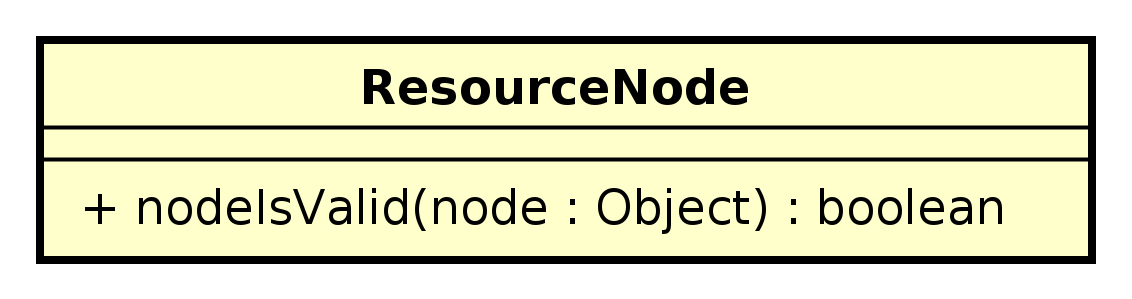
\includegraphics[width=0.3\textwidth]{./img/ResourceNode.png}
		\caption{Diagramma classe ResourceNode}
	\end{figure}
	\item \textbf{descrizione:} rappresenta un nodo di tipo Risorsa;
	\item \textbf{utilizzo:} è contenuto all'interno di Process;
	\item \textbf{metodi:}
	\begin{itemize}
		\item +nodeIsValid() : boolean\newline
		il metodo testa che i parametri con cui il nodo sta per essere creato siano validi
	\end{itemize}
\end{itemize}
\paragraph{SourceNode}
\begin{itemize}
	\begin{figure}[H]
		\centering
		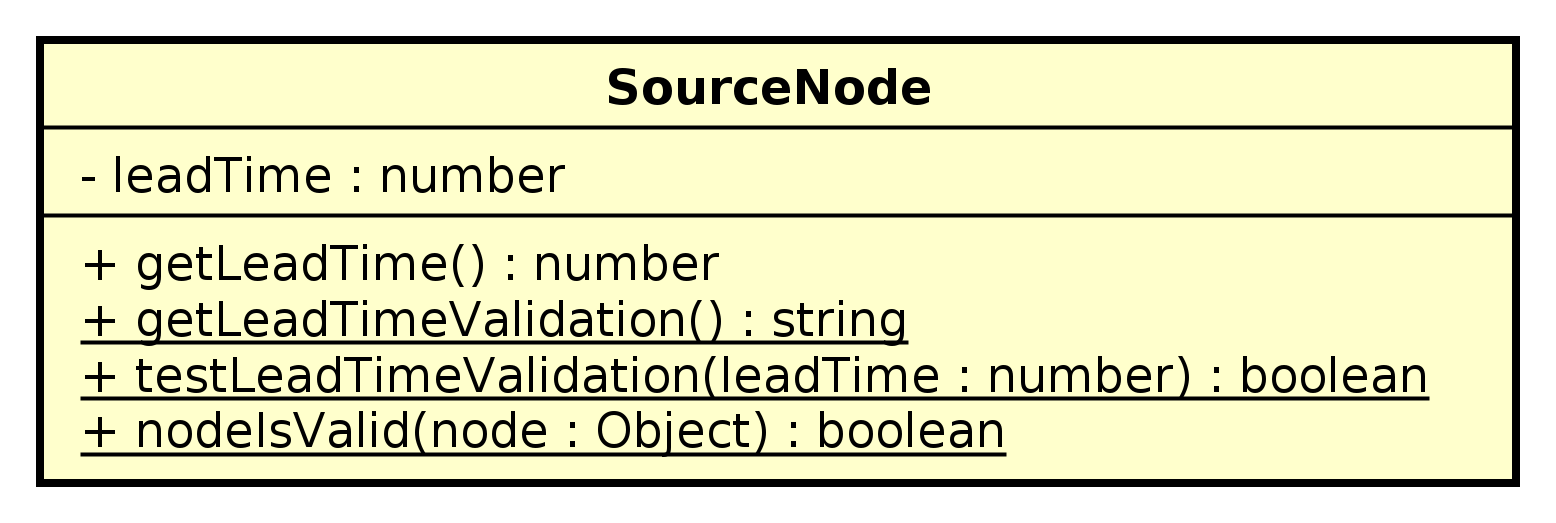
\includegraphics[width=0.3\textwidth]{./img/SourceNode.png}
		\caption{Diagramma classe SourceNode}
	\end{figure}
	\item \textbf{descrizione:} rappresenta un nodo di tipo Sorgente;
	\item \textbf{utilizzo:} è contenuto all'interno di Process;
	\item \textbf{attributi:}
	\begin{itemize}
		\item -leadTime : Object\begin{itemize}
			\item rappresenta il tempo di approvvigionamento del nodo.\end{itemize}
	\end{itemize}
	\item \textbf{metodi:}
	\begin{itemize}
		\item +getLeadTime() : number\newline
		il metodo ritorna il tempo di approvigionamento del nodo
		\item +getLeadTimeValidation() : string\newline
		il metodo ritorna l'espressione regolare che indica una stringa non contenente le seguenti caratteristiche: vuota; più lunga di 5 cifre per la parte intera; più di 2 per la parte decimale;
		\item +nodeIsValid(node) : boolean\newline
		il metodo testa se i parametri con cui il nodo sta per essere creato sono validi
		\begin{itemize}
			\item node : Object\\
			oggetto che rappresenta i parametri con cui il nodo sta per essere creato.
		\end{itemize}
		\item +testLeadTimeValidation(leadTime) : boolean\newline
		il metodo testa se il tempo di approvvigionamento è valido
		\begin{itemize}
			\item leadTime : number\\
			rappresenta il tempo di approvvigionamento.
		\end{itemize}
	\end{itemize}
\end{itemize}
\newpage
\subsection{DeGeOP::StorePkg::PolygonPkg}
\label{pkg::PolygonPkg}
\subsubsection{Informazioni sul package}
\begin{itemize}
	\item \textbf{descrizione:} racchiude le componenti necessarie alla rappresentazione dell'area degli asset e degli scenari di danno;
	\item \textbf{padre:} \hyperref[pkg::StorePkg]{StorePkg};
	\item \textbf{interazioni con altri package:} 
	\begin{itemize}
		\item IN AnalysisPkg: riferimento ad un poligono;
		\item IN ProcessPkg: riferimento ad un poligono.
	\end{itemize}
	\item \textbf{classi contenute:}
	\begin{itemize}
		\item ConcretePolygon;
		\item ConcretePolygonFactory;
		\item Coordinate;
		\item Polygon;
		\item PolygonFactory.
	\end{itemize}
\end{itemize}
\subsubsection{Classi}
\paragraph{ConcretePolygon}
\begin{itemize}
	\begin{figure}[H]
		\centering
		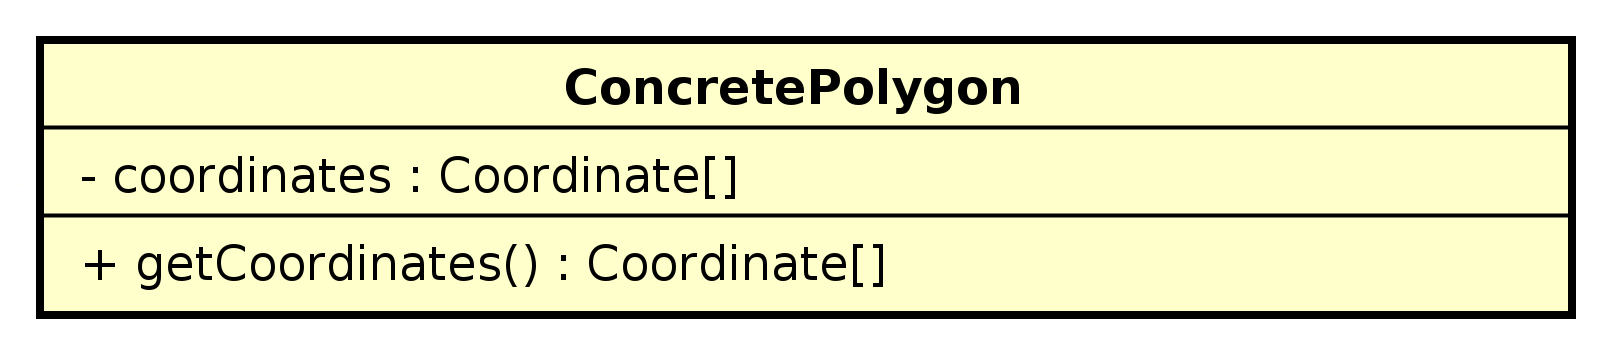
\includegraphics[width=0.3\textwidth]{./img/ConcretePolygon.png}
		\caption{Diagramma classe ConcretePolygon}
	\end{figure}
	\item \textbf{descrizione:} rappresenta un poligono;
	\item \textbf{utilizzo:} viene istanziata da ConcretePolygonFactory; viene utilizzata in Asset e Scenario;
	\item \textbf{attributi:}
	\begin{itemize}
		\item -coordinates : Coordinate[]\begin{itemize}
			\item rappresenta le coordinate che vanno a delineare il poligono.\end{itemize}
	\end{itemize}
	\item \textbf{metodi:}
	\begin{itemize}
		\item +getCoordinates() : Coordinate[]\newline
		il metodo restituisce le coordinate che vanno a delineare il poligono
	\end{itemize}
\end{itemize}
\paragraph{ConcretePolygonFactory}
\begin{itemize}
	\begin{figure}[H]
		\centering
		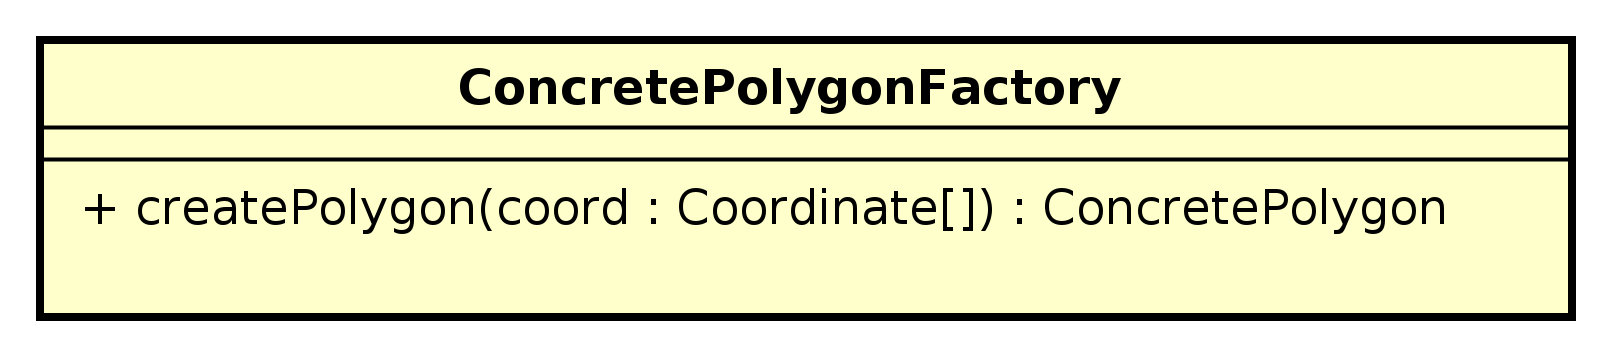
\includegraphics[width=0.3\textwidth]{./img/ConcretePolygonFactory.png}
		\caption{Diagramma classe ConcretePolygonFactory}
	\end{figure}
	\item \textbf{descrizione:} gestisce la creazione concreta dei poligoni;
	\item \textbf{utilizzo:} implementazione di PolygonFactory; è la classe concreta da istanziare per gestire la creazione di un poligono;
	\item \textbf{metodi:}
	\begin{itemize}
		\item +createPolygon() : ConcretePolygon\newline
		il metodo si occupa della costruzione del poligono
	\end{itemize}
\end{itemize}
\paragraph{Coordinate}
\begin{itemize}
	\begin{figure}[H]
		\centering
		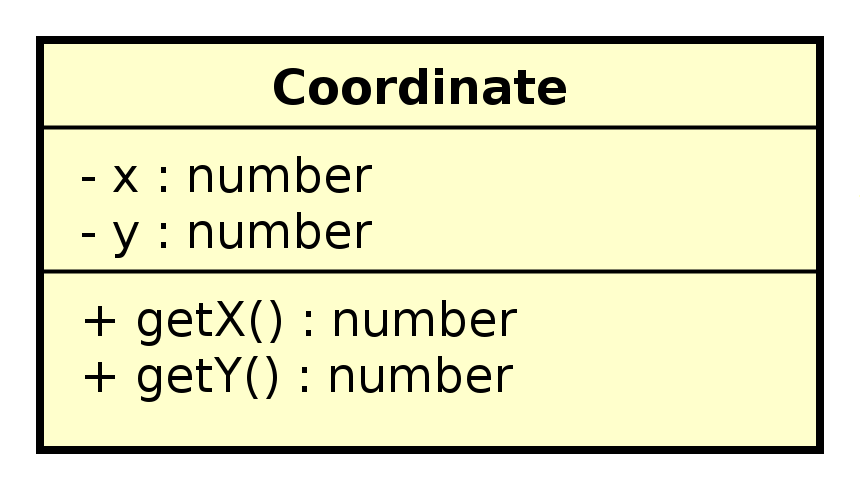
\includegraphics[width=0.3\textwidth]{./img/Coordinate.png}
		\caption{Diagramma classe Coordinate}
	\end{figure}
	\item \textbf{descrizione:} rappresenta una coordinata geografica;
	\item \textbf{utilizzo:} è utilizzata all'interno di Polygon per delimitarne i suoi vertici;
	\item \textbf{attributi:}
	\begin{itemize}
		\item -x : number\begin{itemize}
			\item rappresenta la latitudine di una coordinata geografica.\end{itemize}
		\item -y : number\begin{itemize}
			\item rappresenta la longitudine di una coordinata geografica.\end{itemize}
	\end{itemize}
	\item \textbf{metodi:}
	\begin{itemize}
		\item +getX() : number\newline
		restituisce la latitudine della coordinata geografica
		\item +getY() : number\newline
		restituisce la longitudine della coordinata geografica
	\end{itemize}
\end{itemize}
\paragraph{Polygon}
\begin{itemize}
	\begin{figure}[H]
		\centering
		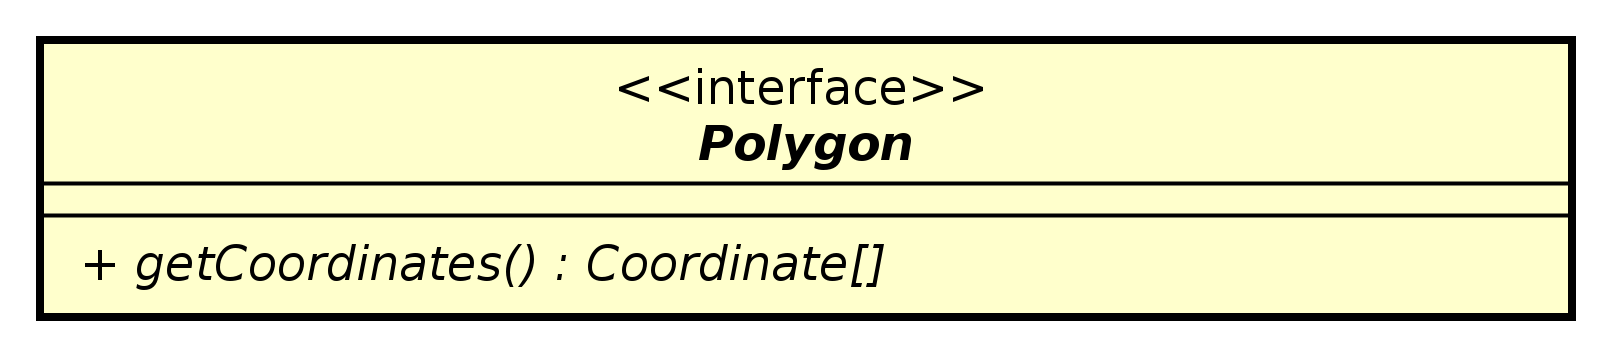
\includegraphics[width=0.3\textwidth]{./img/Polygon.png}
		\caption{Diagramma classe Polygon}
	\end{figure}
	\item \textbf{descrizione:} interfaccia che rappresenta il poligono;
	\item \textbf{utilizzo:} fornisce i metodi del poligono;
	\item \textbf{metodi:}
	\begin{itemize}
		\item +getCoordinates() : Coordinate[]\newline
		il metodo restituisce un array di coordinate
	\end{itemize}
\end{itemize}
\paragraph{PolygonFactory}
\begin{itemize}
	\begin{figure}[H]
		\centering
		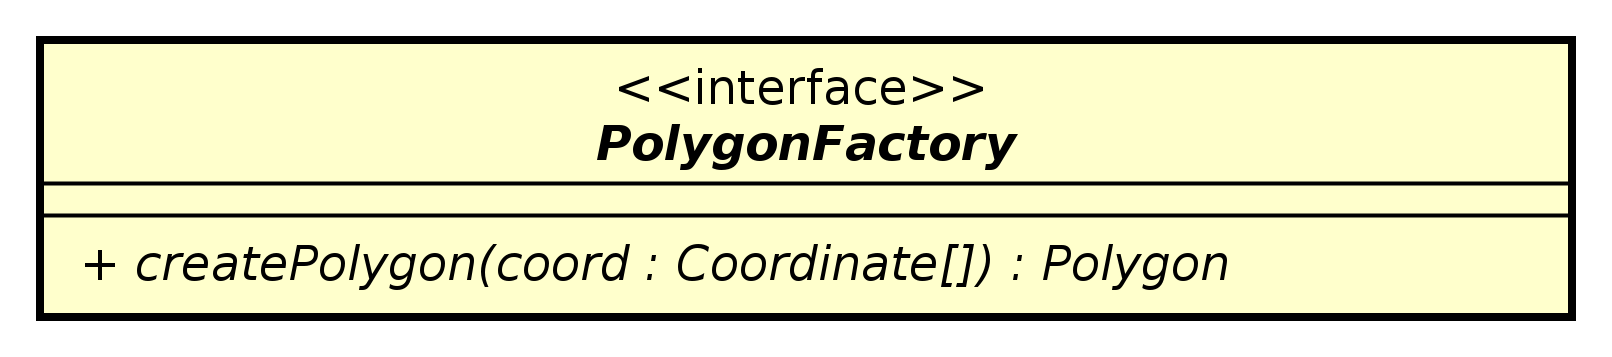
\includegraphics[width=0.3\textwidth]{./img/PolygonFactory.png}
		\caption{Diagramma classe PolygonFactory}
	\end{figure}
	\item \textbf{descrizione:} interfaccia che si occupa della costruzione dei poligoni;
	\item \textbf{utilizzo:} viene usata dalle classi Scenario e Asset per la costruzione dei poligoni;
	\item \textbf{metodi:}
	\begin{itemize}
		\item +createPolygon(coord) : Polygon\newline
		il metodo si occupa della costruzione del poligono
		\begin{itemize}
			\item coord : Coordinate[]\\
			raccoglie le coordinate necessarie alla costruzione dei poligoni
			.
		\end{itemize}
	\end{itemize}
\end{itemize}
\newpage
\subsection{DeGeOP::ReducerPkg}
\label{pkg::ReducerPkg}
\begin{figure}[H]
	\centering
	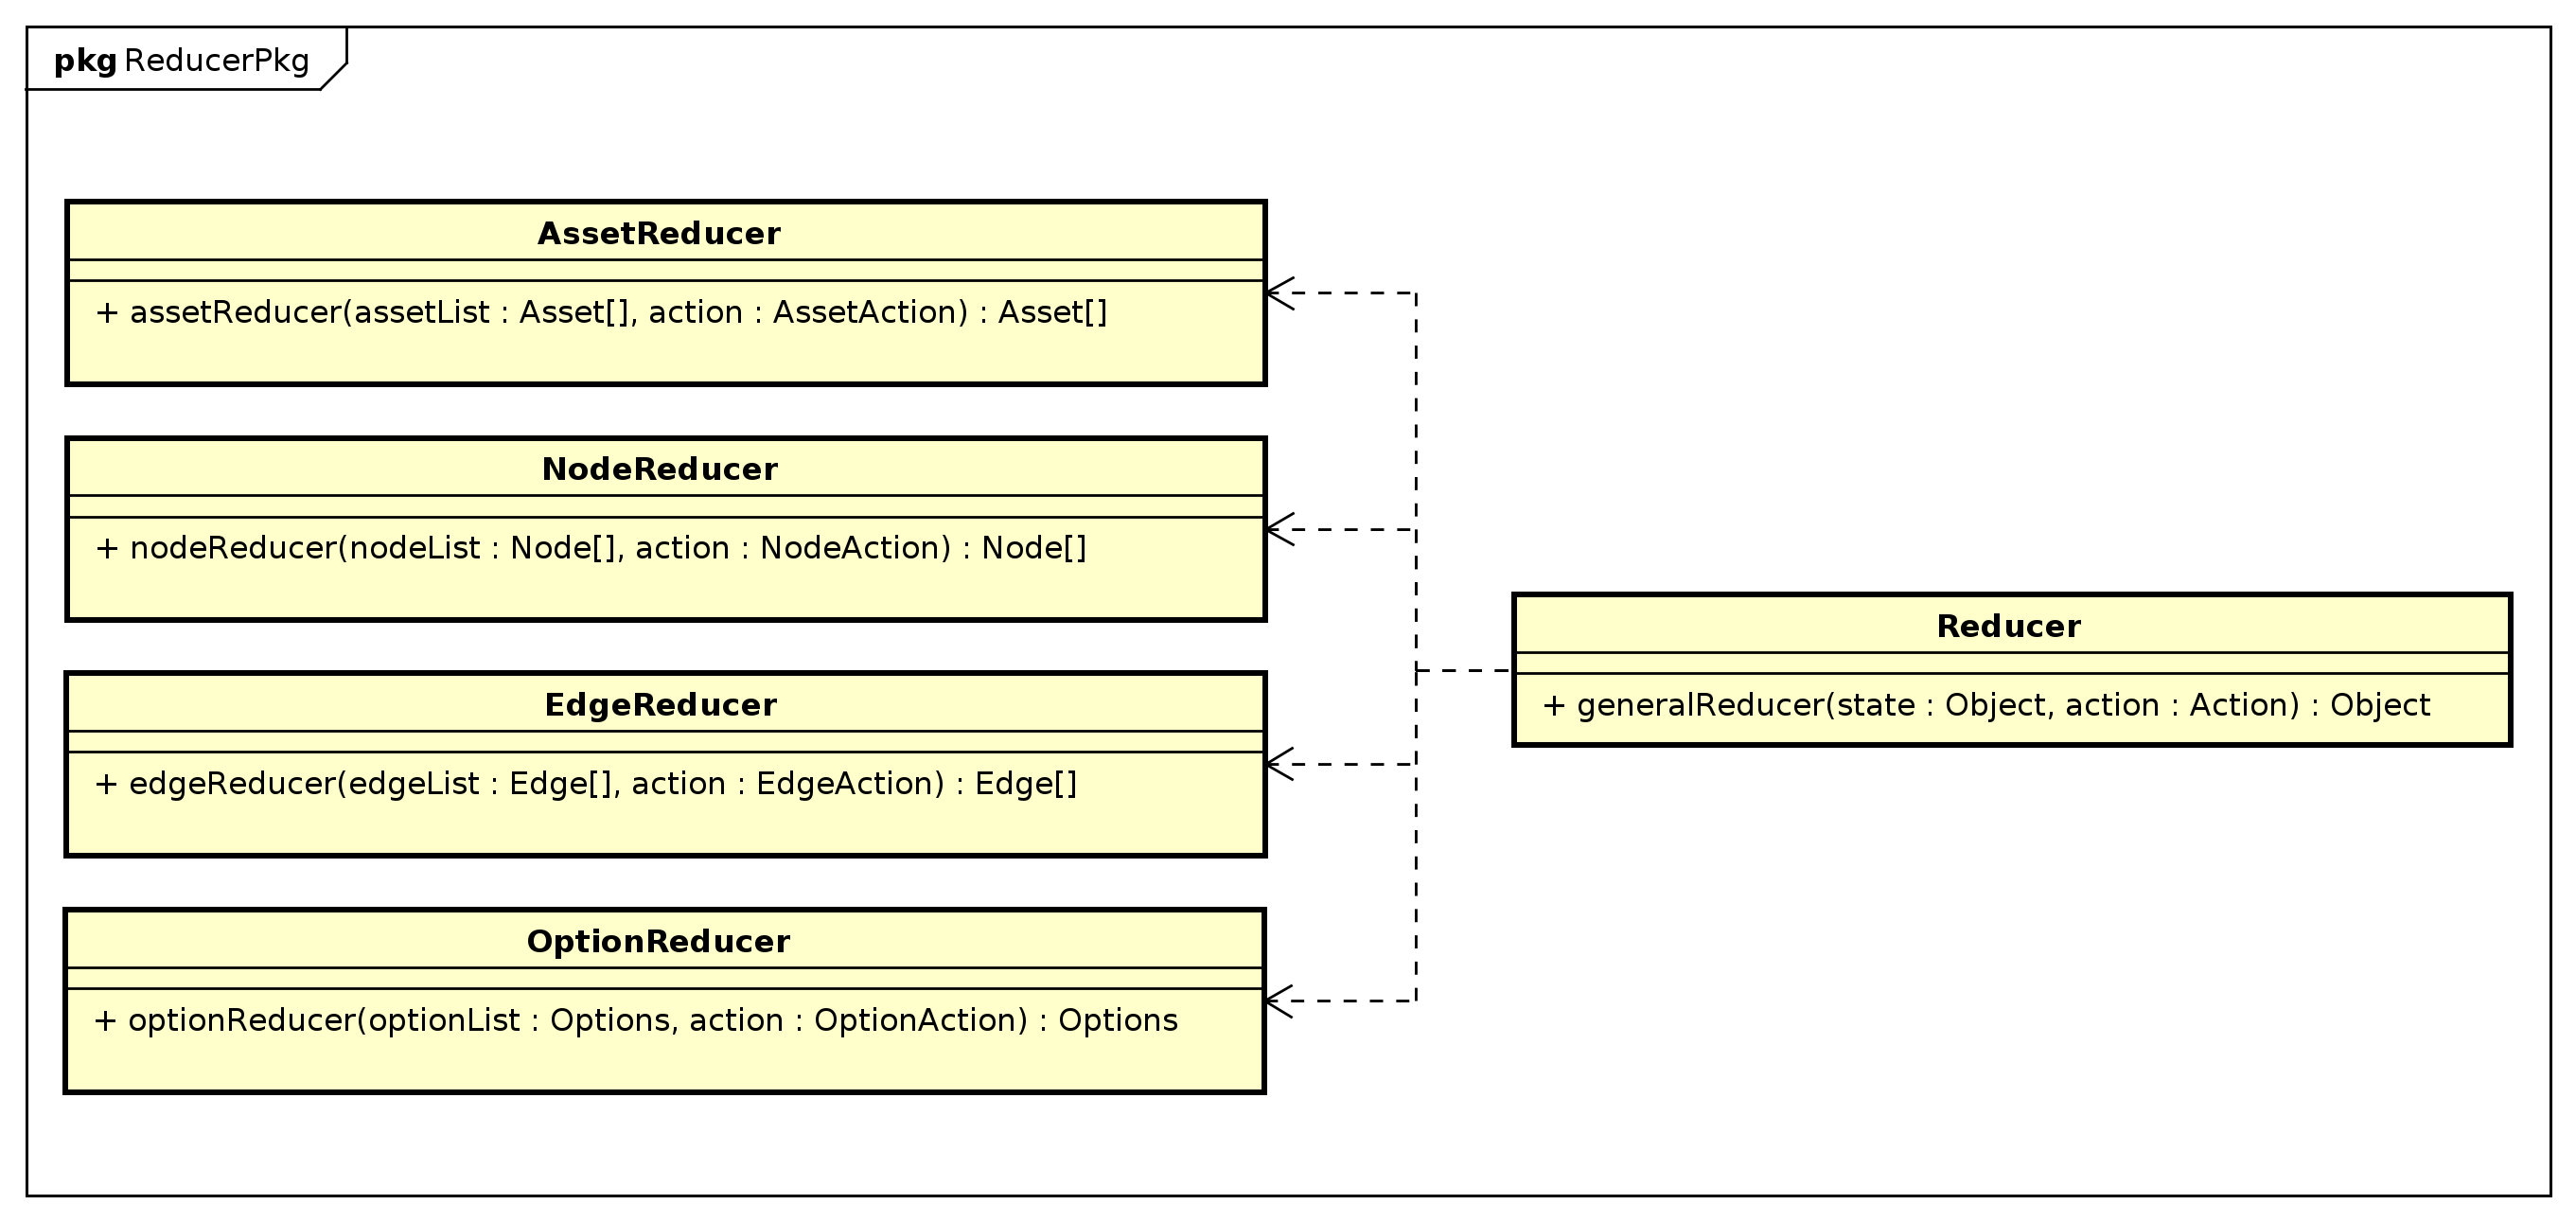
\includegraphics[width=\textwidth]{img/PkgDiagram/ReducerPkg.png}
	\caption{Schema componente DeGeOP::ReducerPkg}
\end{figure}
\subsubsection{Informazioni sul package}
\begin{itemize}
	\item \textbf{descrizione:} racchiude le componenti necessarie all'implementazione dei reducer secondo l'architettura Redux;
	\item \textbf{padre:} \hyperref[pkg::DeGeOP]{DeGeOP};
	\item \textbf{interazioni con altri package:} 
	\begin{itemize}
		\item OUT ActionPkg: utilizzo di azioni ;
		\item OUT StorePkg: applicazione di cambiamenti di stato.
	\end{itemize}
	\item \textbf{classi contenute:}
	\begin{itemize}
		\item AssetReducer;
		\item EdgeReducer;
		\item NodeReducer;
		\item OptionReducer;
		\item Reducer.
	\end{itemize}
\end{itemize}
\subsubsection{Classi}
\paragraph{AssetReducer}
\begin{itemize}
	\begin{figure}[H]
		\centering
		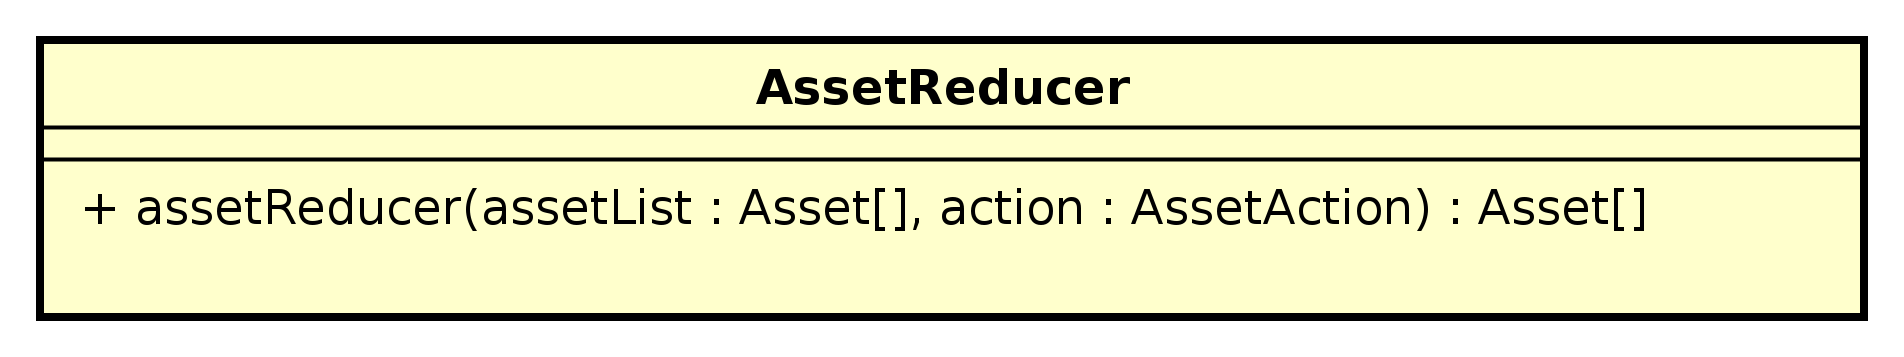
\includegraphics[width=0.3\textwidth]{./img/AssetReducer.png}
		\caption{Diagramma classe AssetReducer}
	\end{figure}
	\item \textbf{descrizione:} rappresenta il reducer dell'asset;
	\item \textbf{utilizzo:} il suo metodo gestisce le operazioni sullo store riguardanti l'asset;
	\item \textbf{metodi:}
	\begin{itemize}
		\item +assetReducer(action, assetList) : Asset[ ]\newline
		il metodo gestisce le operazioni sullo store riguardanti l'asset e ritorna la nuova lista di asset ottenuta a seguito della modifica
		\begin{itemize}
			\item action : AssetAction\\
			rappresenta un'azione che descrive i cambiamenti da effettuare sullo stato.
			\item assetList : Asset[ ]\\
			rappresenta una lista di asset, che sono il vecchio stato.
		\end{itemize}
	\end{itemize}
	\item \textbf{relazioni con altre classi:} 
	\begin{itemize}
		\item OUT Asset.
	\end{itemize}
\end{itemize}
\paragraph{EdgeReducer}
\begin{itemize}
	\begin{figure}[H]
		\centering
		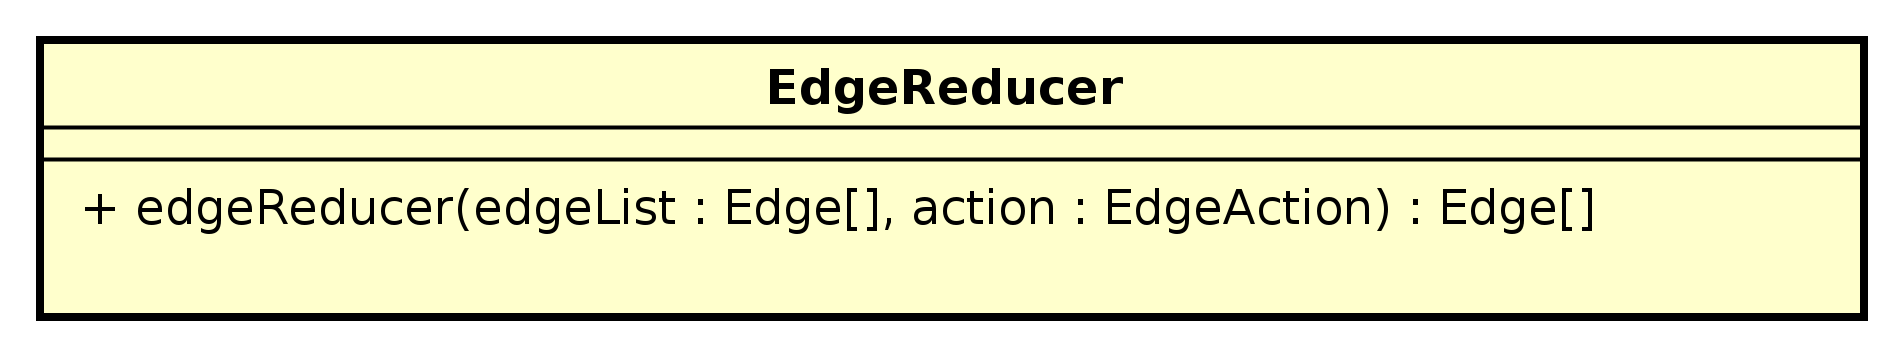
\includegraphics[width=0.3\textwidth]{./img/EdgeReducer.png}
		\caption{Diagramma classe EdgeReducer}
	\end{figure}
	\item \textbf{descrizione:} rappresenta il reducer dell'arco;
	\item \textbf{utilizzo:} il suo metodo gestisce le operazioni sullo store riguardanti gli archi;
	\item \textbf{metodi:}
	\begin{itemize}
		\item +edgeReducer(action, edgeList) : Edge [ ]\newline
		il metodo gestisce le operazioni sullo store riguardanti gli archi e ritorna la nuova lista di archi ottenuta a seguito della modifica
		\begin{itemize}
			\item action : EdgeAction\\
			rappresenta un'azione che descrive i cambiamenti da effettuare sullo stato.
			\item edgeList : Edge [ ]\\
			rappresenta una lista di archi, che sono il vecchio stato.
		\end{itemize}
	\end{itemize}
	\item \textbf{relazioni con altre classi:} 
	\begin{itemize}
		\item OUT Edge.
	\end{itemize}
\end{itemize}
\paragraph{NodeReducer}
\begin{itemize}
	\begin{figure}[H]
		\centering
		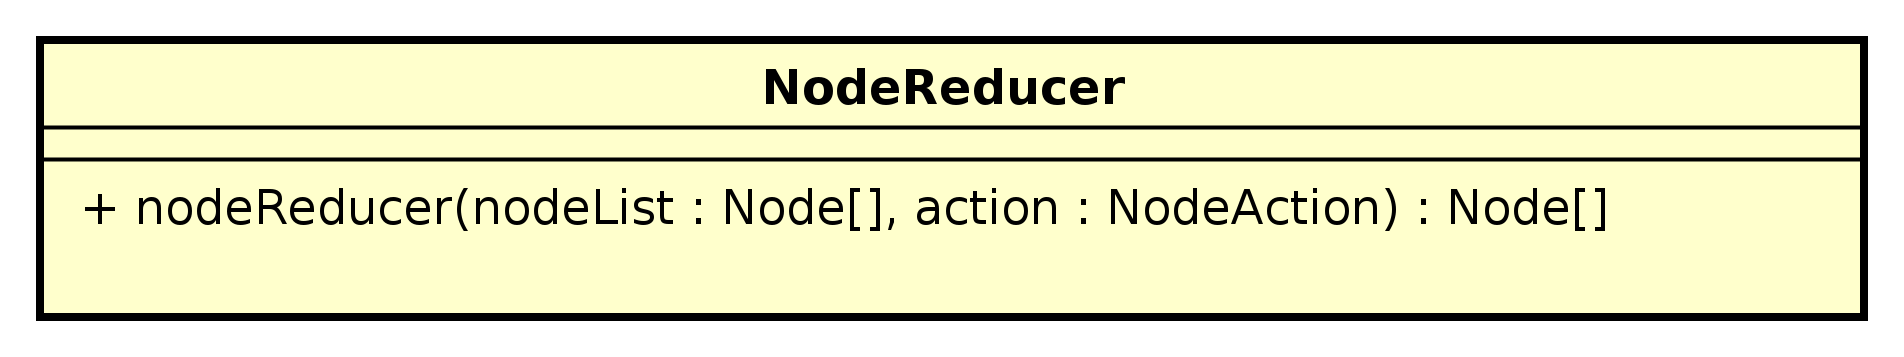
\includegraphics[width=0.3\textwidth]{./img/NodeReducer.png}
		\caption{Diagramma classe NodeReducer}
	\end{figure}
	\item \textbf{descrizione:} rappresenta il reducer del nodo;
	\item \textbf{utilizzo:} il suo metodo gestisce le operazioni sullo store riguardanti i nodi;
	\item \textbf{metodi:}
	\begin{itemize}
		\item +nodeReducer(action, nodeList) : Node [ ]\newline
		il metodo gestisce le operazioni sullo store riguardanti i nodi e ritorna la nuova lista di nodi ottenuta a seguito della modifica
		\begin{itemize}
			\item action : EdgeAction\\
			rappresenta un'azione che descrive i cambiamenti da effettuare sullo stato.
			\item nodeList : Node [ ]\\
			rappresenta una lista di nodi, che sono il vecchio stato.
		\end{itemize}
	\end{itemize}
	\item \textbf{relazioni con altre classi:} 
	\begin{itemize}
		\item OUT Node.
	\end{itemize}
\end{itemize}
\paragraph{OptionReducer}
\begin{itemize}
	\begin{figure}[H]
		\centering
		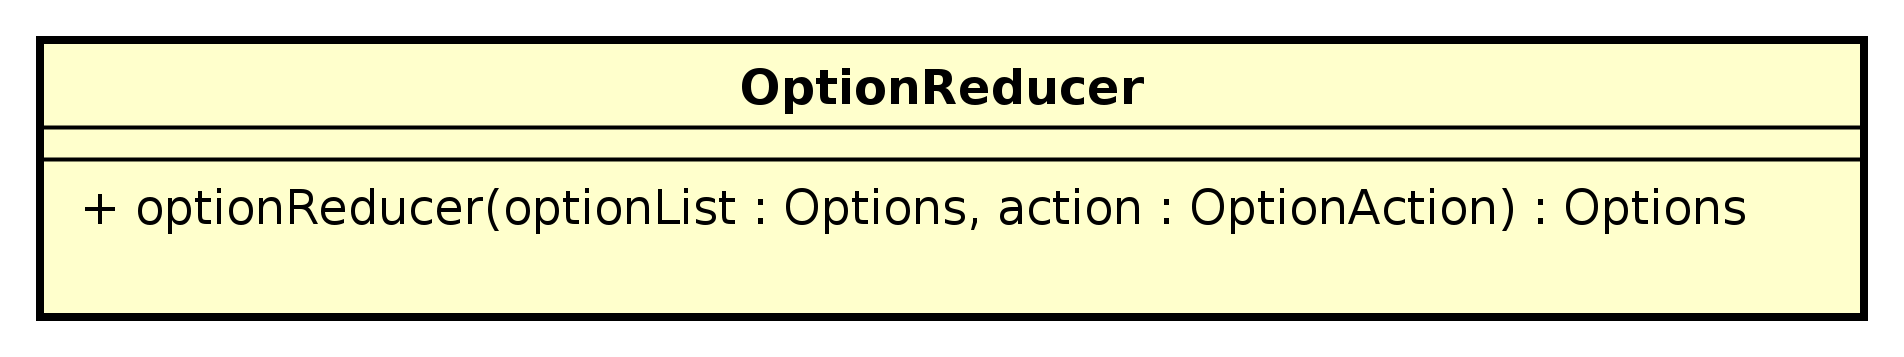
\includegraphics[width=0.3\textwidth]{./img/OptionReducer.png}
		\caption{Diagramma classe OptionReducer}
	\end{figure}
	\item \textbf{descrizione:} rappresenta il reducer delle option;
	\item \textbf{utilizzo:} il suo metodo gestisce le operazioni sullo store riguardanti l'asset;
	\item \textbf{metodi:}
	\begin{itemize}
		\item +optionReducer(action, optionList) : Options\newline
		il metodo gestisce le operazioni sullo store riguardanti l'asset e ritorna la nuova lista di asset ottenuta a seguito della modifica
		\begin{itemize}
			\item action : OptionAction\\
			rappresenta un'azione che descrive i cambiamenti da effettuare sullo stato.
			\item optionList : Options\\
			rappresenta la lista delle option.
		\end{itemize}
	\end{itemize}
	\item \textbf{relazioni con altre classi:} 
	\begin{itemize}
		\item IN Reducer;
		\item OUT Options.
	\end{itemize}
\end{itemize}
\paragraph{Reducer}
\begin{itemize}
	\begin{figure}[H]
		\centering
		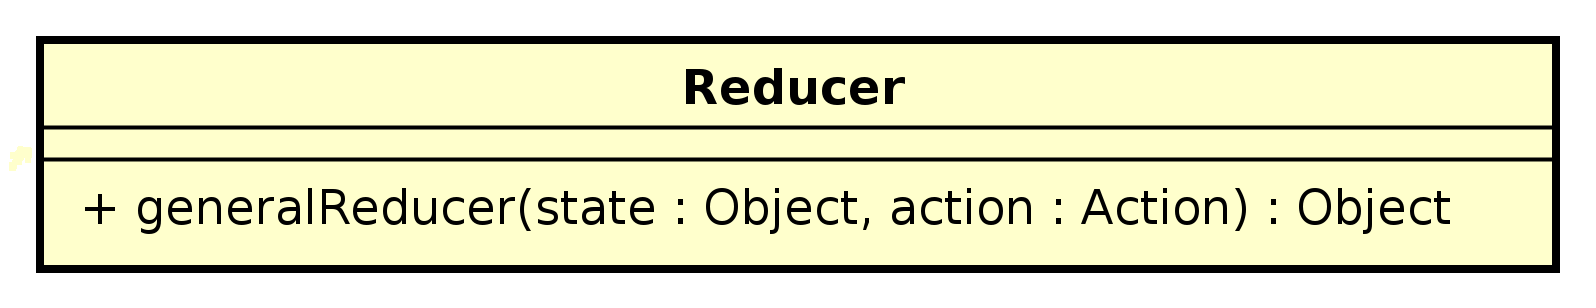
\includegraphics[width=0.3\textwidth]{./img/Reducer.png}
		\caption{Diagramma classe Reducer}
	\end{figure}
	\item \textbf{descrizione:} accetta una action generica in input e la reindirizza al giusto reducer;
	\item \textbf{utilizzo:} il suo metodo viene utilizzato per catturare un'azione e generare un nuovo stato sullo Store;
	\item \textbf{metodi:}
	\begin{itemize}
		\item +generalReducer() : Object\newline
		Esegue l'azione sullo stato corrente dello store e ne ritorna il nuovo stato
	\end{itemize}
	\item \textbf{relazioni con altre classi:} 
	\begin{itemize}
		\item OUT OptionReducer;
		\item OUT StoreDeGeOP.
	\end{itemize}
\end{itemize}
\newpage
\subsection{DeGeOP::CallManagerPkg}
\label{pkg::CallManagerPkg}
\begin{figure}[H]
	\centering
	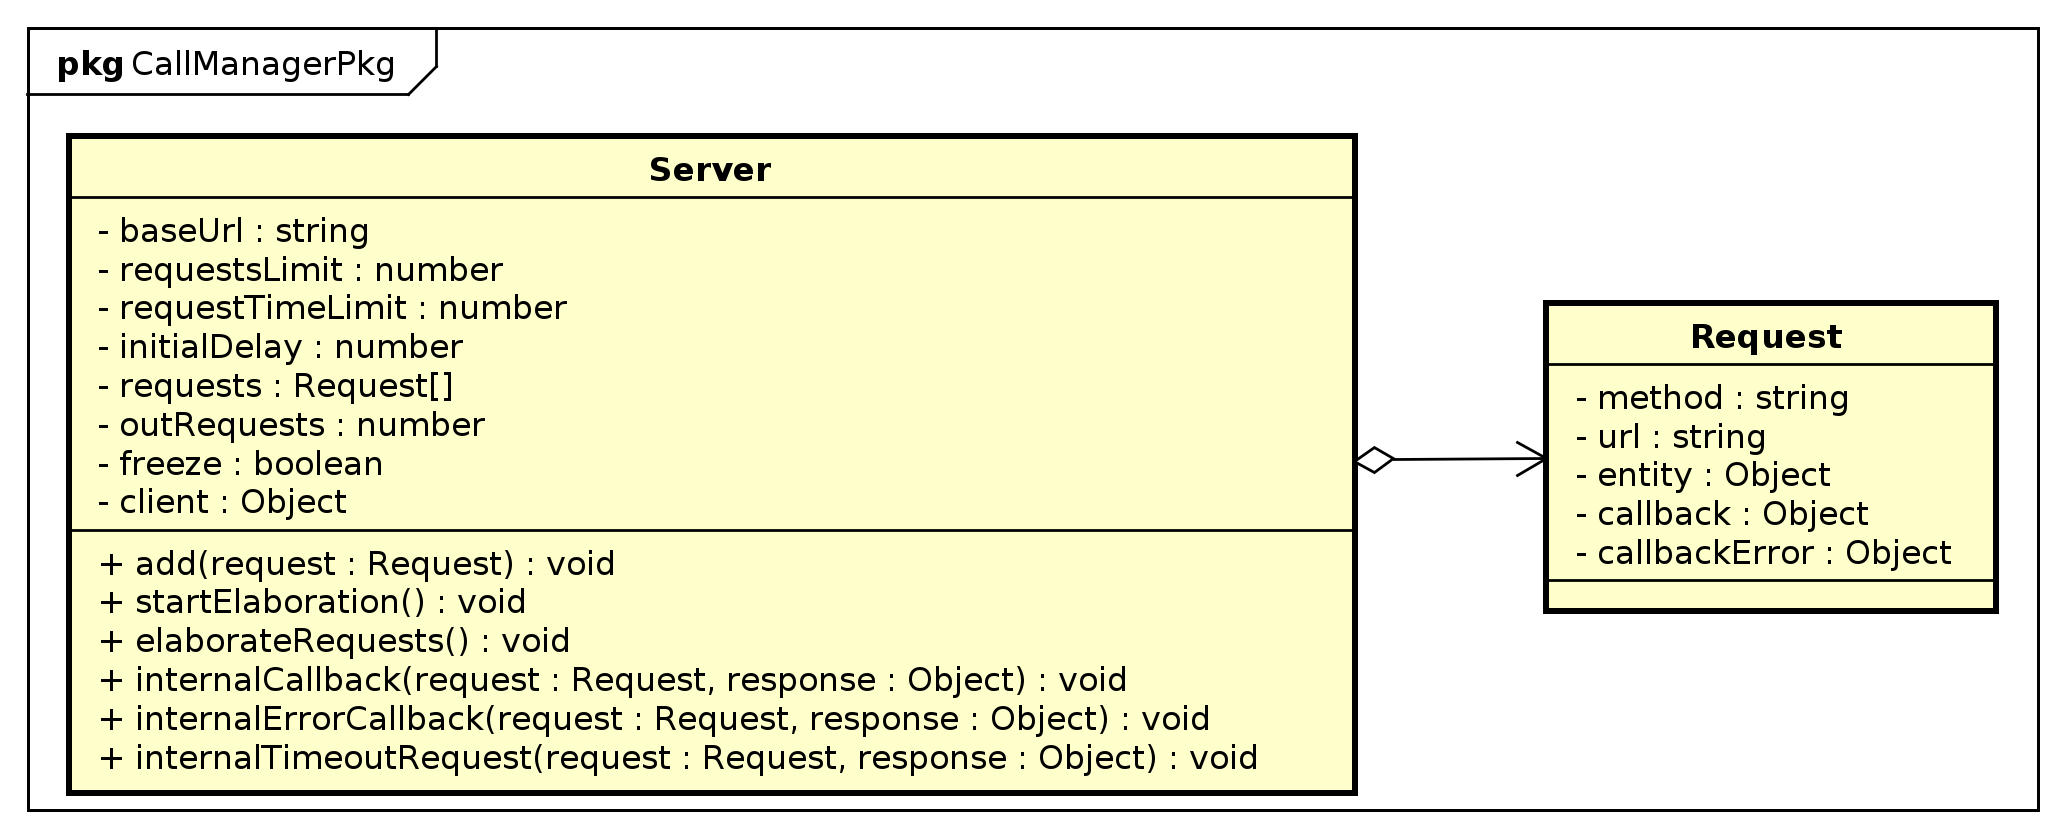
\includegraphics[width=\textwidth]{img/PkgDiagram/CallManagerPkg.png}
	\caption{Schema componente DeGeOP::CallManagerPkg}
\end{figure}
\subsubsection{Informazioni sul package}
\begin{itemize}
	\item \textbf{descrizione:} racchiude le componenti necessarie alla comunicazione dei dati verso il server;
	\item \textbf{padre:} \hyperref[pkg::DeGeOP]{DeGeOP};
	\item \textbf{interazioni con altri package:} 
	\begin{itemize}
		\item OUT ActionPkg: dispatch di azioni;
		\item OUT StorePkg: subscribe sullo store.
	\end{itemize}
	\item \textbf{classi contenute:}
	\begin{itemize}
		\item Request;
		\item Server.
	\end{itemize}
\end{itemize}
\subsubsection{Classi}
\paragraph{Request}
\begin{itemize}
	\begin{figure}[H]
		\centering
		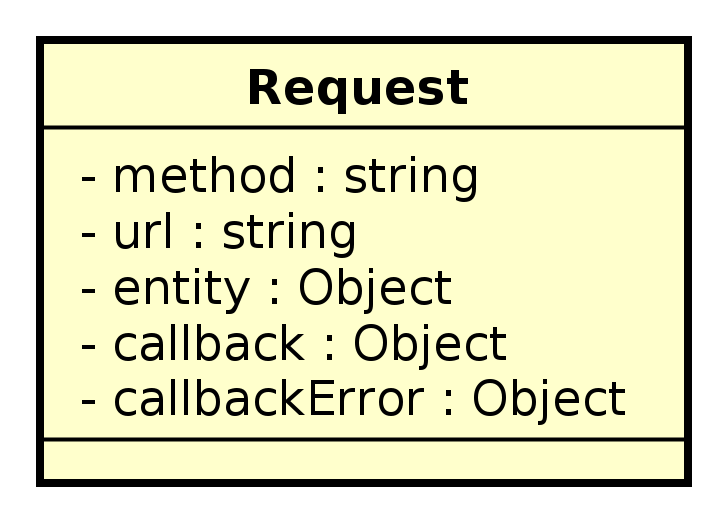
\includegraphics[width=0.3\textwidth]{./img/Request.png}
		\caption{Diagramma classe Request}
	\end{figure}
	\item \textbf{descrizione:} rappresenta i dati necessari per eseguire una richiesta di tipologia REST;
	\item \textbf{utilizzo:} è utilizzata all'interno di Server per gestire la coda delle richieste ;
	\item \textbf{attributi:}
	\begin{itemize}
		\item -callback : Object\begin{itemize}
			\item rappresenta la funzione che viene invocata se la richiesta è andata a buon fine.\end{itemize}
		\item -callbackError : Object\begin{itemize}
			\item rappresenta la funzione che viene invocata se la richiesta non è andata a buon fine.\end{itemize}
		\item -entity : Object\begin{itemize}
			\item rappresnta il payload della richiesta.\end{itemize}
		\item -method : string\begin{itemize}
			\item rappresenta il verbo http con cui si esegue la richiesta.\end{itemize}
		\item -url : string\begin{itemize}
			\item rappresenta l'url verso cui eseguire la richiesta.\end{itemize}
	\end{itemize}
\end{itemize}
\paragraph{Server}
\begin{itemize}
	\begin{figure}[H]
		\centering
		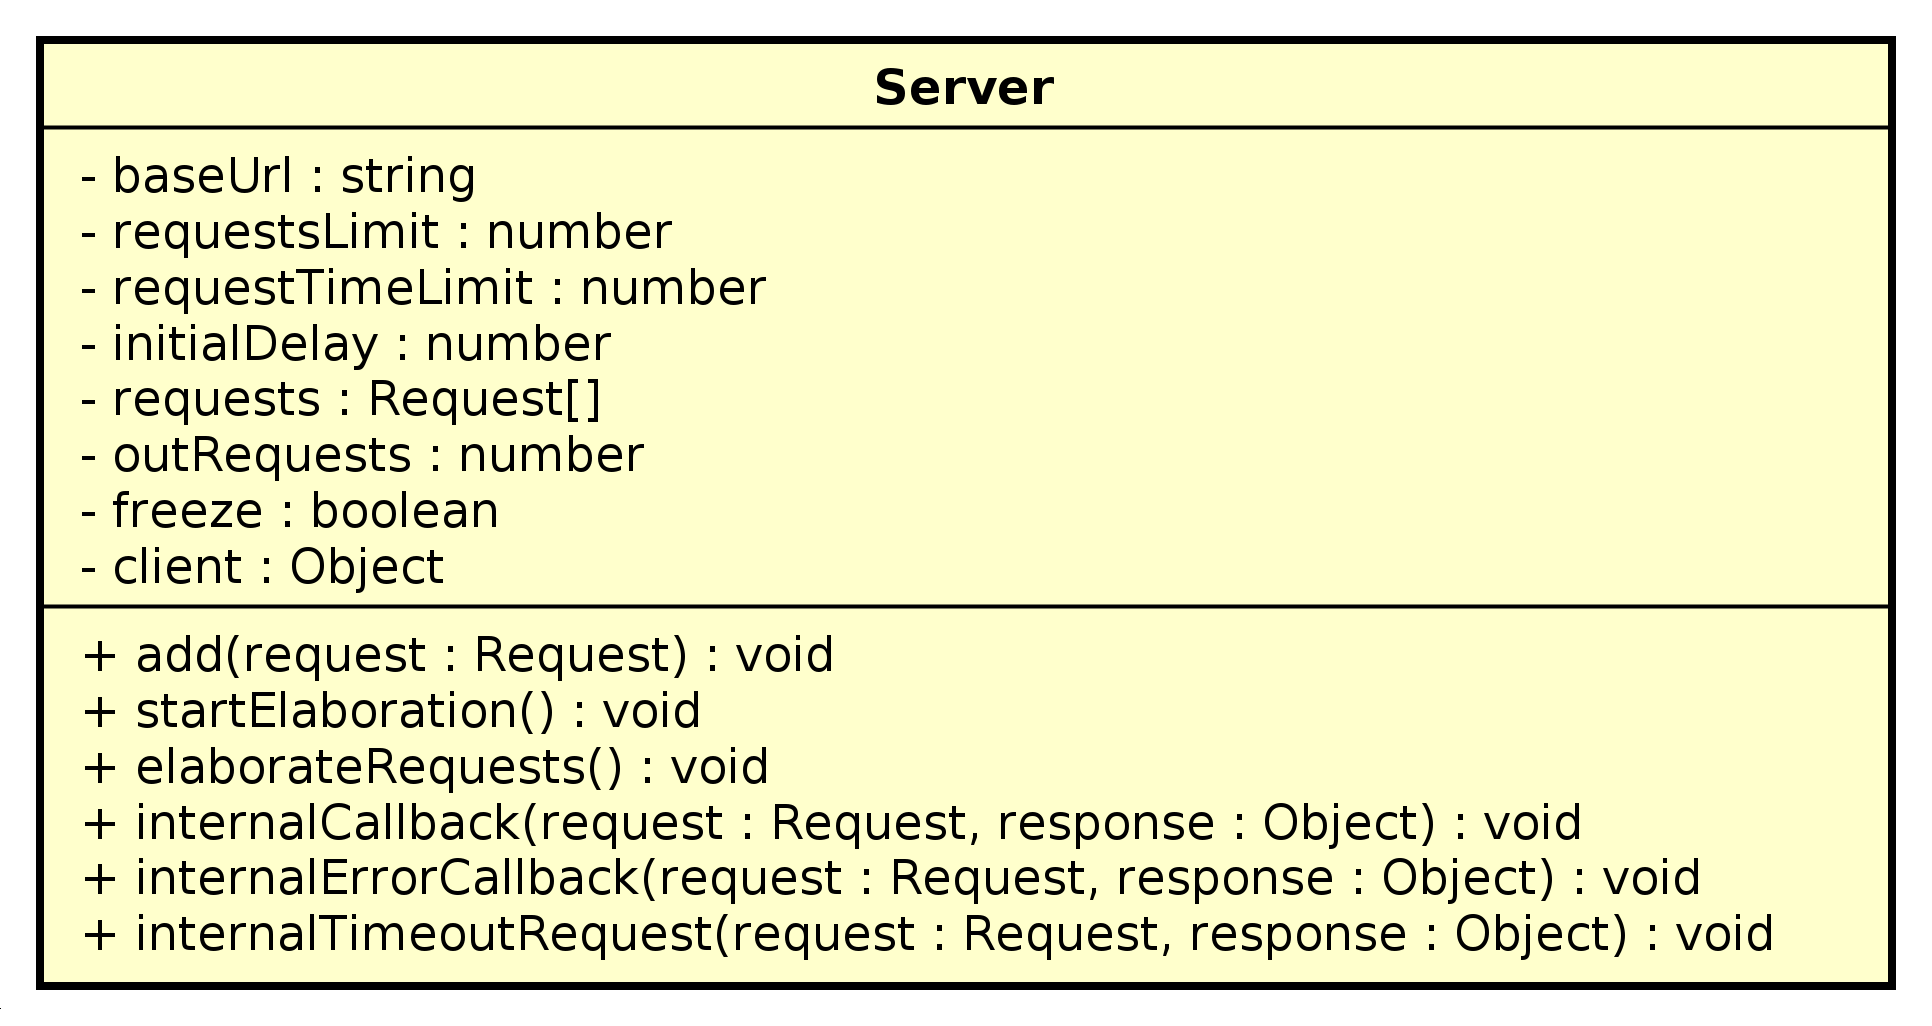
\includegraphics[width=0.3\textwidth]{./img/Server.png}
		\caption{Diagramma classe Server}
	\end{figure}
	\item \textbf{descrizione:} rappresenta il gestore delle chiamate REST;
	\item \textbf{utilizzo:} è utilizzato come buffer per gestire le richieste in uscita e le risposte ricevute;
	\item \textbf{attributi:}
	\begin{itemize}
		\item -baseUrl : string\begin{itemize}
			\item URL http verso cui devono essere inviate le richieste.\end{itemize}
		\item -client : Object\begin{itemize}
			\item gestisce l'invio delle richieste e la ricezione delle risposte.\end{itemize}
		\item -freeze : boolean\begin{itemize}
			\item viene utilizzata per bloccare il server in caso di collegamento mancante.\end{itemize}
		\item -initialDelay : number\begin{itemize}
			\item rappresenta il tempo in millisecondi passato il quale una richiesta scaduta viene eseguita nuovamente.\end{itemize}
		\item -outRequests : number\begin{itemize}
			\item rappresenta il numero delle richieste attualmente in attesa di risposta.\end{itemize}
		\item -requests : Request[]\begin{itemize}
			\item lista delle richieste da evadere.\end{itemize}
		\item -requestsLimit : number\begin{itemize}
			\item rappresenta il numero massimo di richieste eseguite ancora in attesa di risposta.\end{itemize}
		\item -timeLimitRequest : number\begin{itemize}
			\item rappresenta il tempo in millisecondi dopo cui considerare la richiesta scaduta.\end{itemize}
	\end{itemize}
	\item \textbf{metodi:}
	\begin{itemize}
		\item +add(request) : void\newline
		aggiunge una richiesta alla coda del server
		\begin{itemize}
			\item request : Request\\
			rappresenta la richiesta da aggiungere alla coda server.
		\end{itemize}
		\item +elaborateRequests() : void\newline
		elabora la coda della richieste fino a quando ci sono elementi presenti
		\item +internalCallback(request, response) : void\newline
		esegue la chiamata alla funzione di callback fornita dalla richiesta nel caso in cui questa abbia ricevuto una risposta senza errori
		\begin{itemize}
			\item request : Request\\
			rappresenta la richiesta che è stata inviata.
			\item response : Object\\
			oggetto che rappresenta la risposta alla richiesta inviata.
		\end{itemize}
		\item +internalErrorCallback(request, response) : void\newline
		esegue la chiamata alla funzione di callback fornita dalla richiesta nel caso in cui questa abbia ricevuto una risposta con errori
		\begin{itemize}
			\item request : Request\\
			rappresenta la richiesta che è stata inviata.
			\item response : Object\\
			oggetto che rappresenta la risposta alla richiesta inviata.
		\end{itemize}
		\item +internalTimeoutRequest(response) : void\newline
		gestisce la richiesta nel caso in cui questa abbia non abbia ricevuto alcuna risposta entro il tempo di timeout
		\begin{itemize}
			\item response : Object\\
			oggetto che rappresenta la risposta alla richiesta inviata.
		\end{itemize}
		\item +startElaboration() : void\newline
		inizia l'esecuzione delle richieste in attesa di essere evase
	\end{itemize}
\end{itemize}
\newpage
\subsection{DeGeOP::ActionPkg}
\label{pkg::ActionPkg}
\begin{figure}[H]
	\centering
	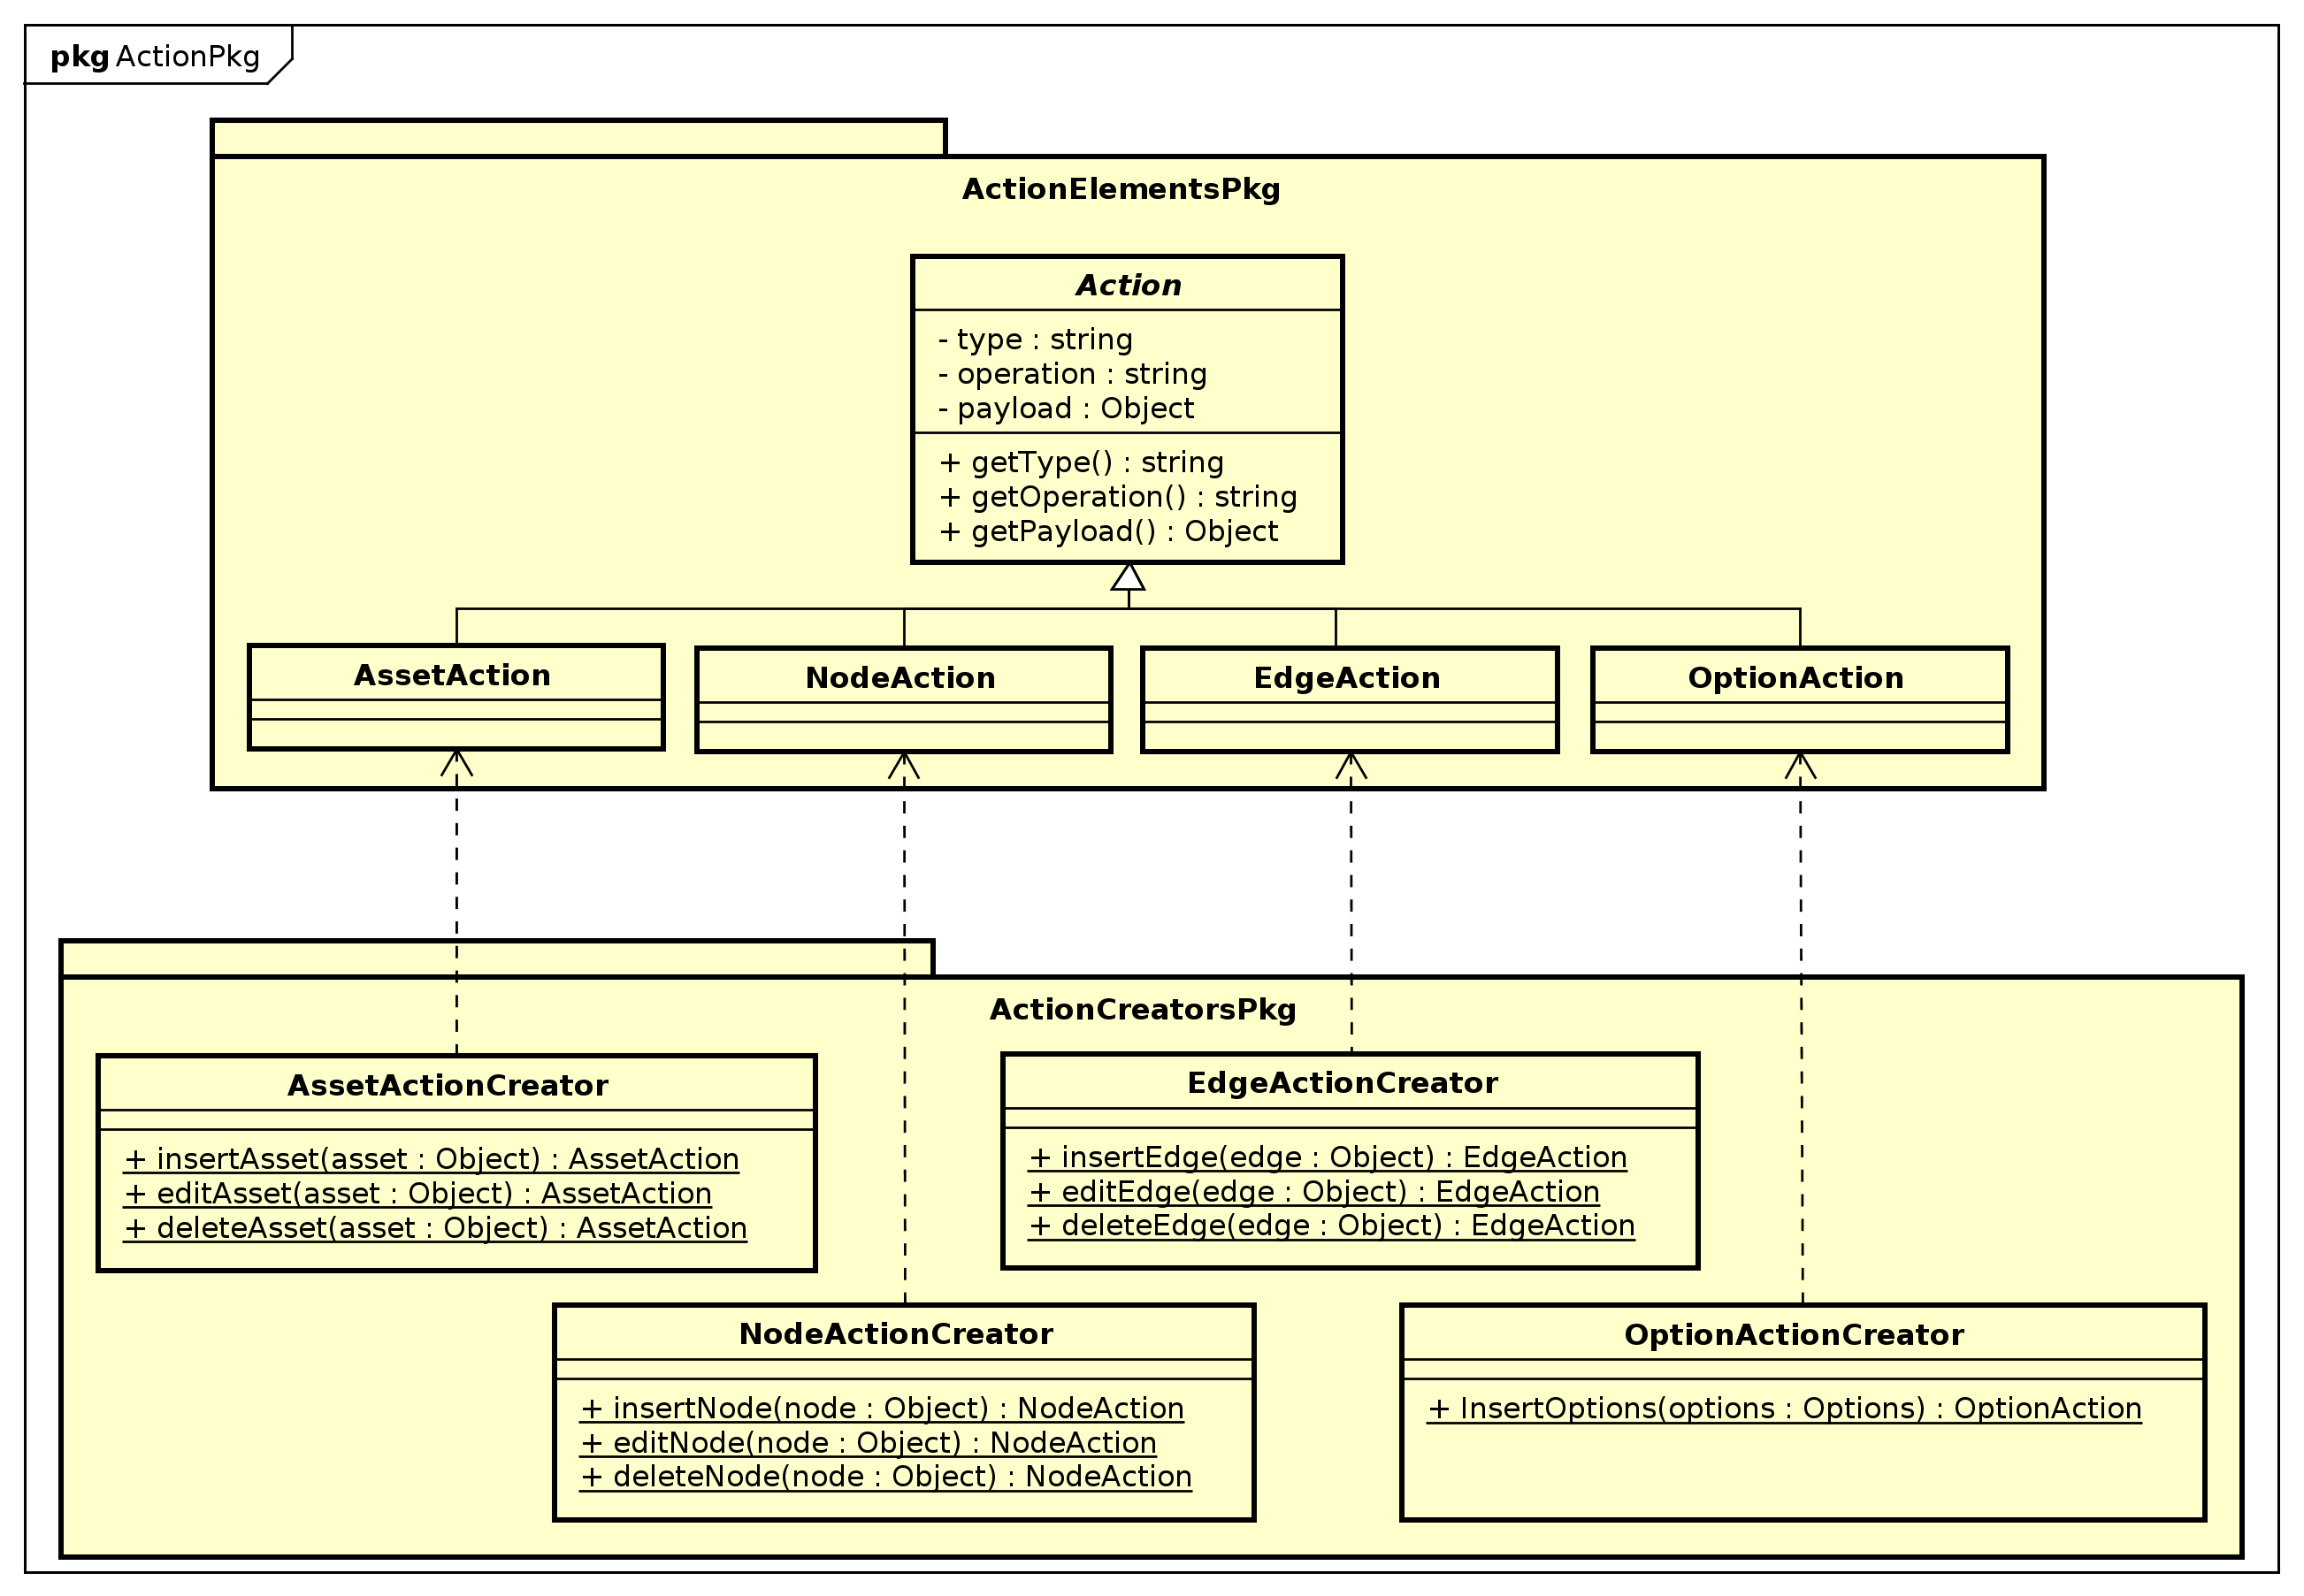
\includegraphics[width=\textwidth]{img/PkgDiagram/ActionPkg.png}
	\caption{Schema componente DeGeOP::ActionPkg}
\end{figure}
\subsubsection{Informazioni sul package}
\begin{itemize}
	\item \textbf{descrizione:} racchiude le componenti utilizzate per implementare le action dell'architettura Redux. Le action vengono create e ne viene fatto il dispatch verso lo store. Un reducer gestirà una action per produrre un cambiamento di stato sullo store;
	\item \textbf{padre:} \hyperref[pkg::DeGeOP]{DeGeOP};
	\item \textbf{package contenuti:}
	\begin{itemize}
		\item ActionPkg::\hyperref[pkg::ActionCreatorsPkg]{ActionCreatorsPkg};
		\item ActionPkg::\hyperref[pkg::ActionElementsPkg]{ActionElementsPkg}.
	\end{itemize}
	\item \textbf{interazioni con altri package:} 
	\begin{itemize}
		\item IN CallManagerPkg: dispatch di azioni;
		\item IN ReducerPkg: utilizzo di azioni ;
		\item IN ViewPkg: dispatch di azioni.
	\end{itemize}
	\item \textbf{classi contenute:}
	\begin{itemize}
		\item EdgeAction.
	\end{itemize}
\end{itemize}
\subsubsection{Classi}
\paragraph{EdgeAction}
\begin{itemize}
	\begin{figure}[H]
		\centering
		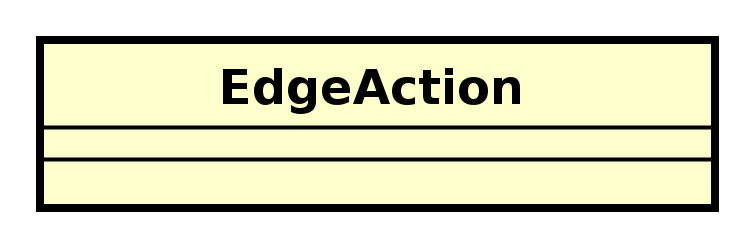
\includegraphics[width=0.3\textwidth]{./img/EdgeAction.png}
		\caption{Diagramma classe EdgeAction}
	\end{figure}
	\item \textbf{descrizione:} rappresenta un'azione relativa agli archi;
	\item \textbf{utilizzo:} l'azione viene creata da un apposito ActionCreator per essere poi inviata ad un reducer.
\end{itemize}
\newpage
\subsection{DeGeOP::ActionPkg::ActionElementsPkg}
\label{pkg::ActionElementsPkg}
\subsubsection{Informazioni sul package}
\begin{itemize}
	\item \textbf{descrizione:} racchiude le componenti che rappresentano effettivamente le azioni;
	\item \textbf{padre:} \hyperref[pkg::ActionPkg]{ActionPkg};
	\item \textbf{interazioni con altri package:} 
	\begin{itemize}
		\item IN ActionCreatorsPkg: creazione di azioni.
	\end{itemize}
	\item \textbf{classi contenute:}
	\begin{itemize}
		\item Action;
		\item AssetAction;
		\item NodeAction;
		\item OptionAction.
	\end{itemize}
\end{itemize}
\subsubsection{Classi}
\paragraph{Action}
\begin{itemize}
	\begin{figure}[H]
		\centering
		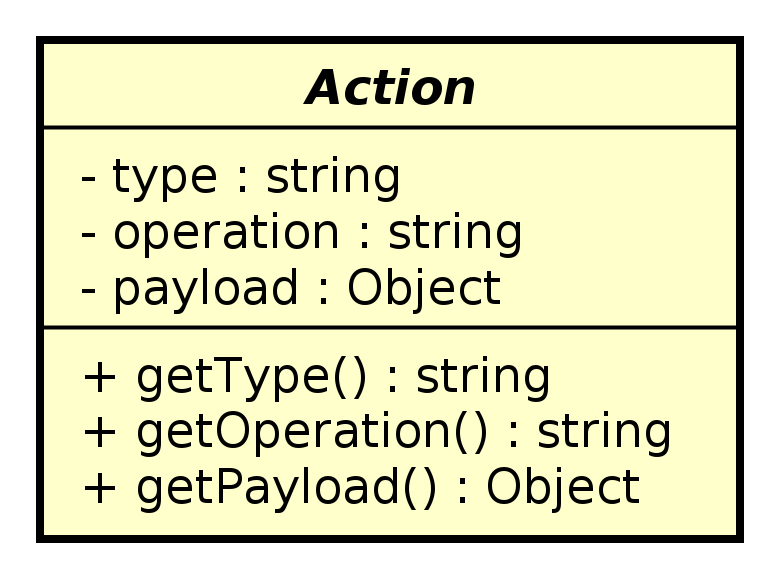
\includegraphics[width=0.3\textwidth]{./img/Action.png}
		\caption{Diagramma classe Action}
	\end{figure}
	\item \textbf{descrizione:} una classe astratta che rappresenta una generica azione di cui può essere fatto il dispatch;
	\item \textbf{utilizzo:} i suoi membri vengono usati dai reducer per completare una azione;
	\item \textbf{attributi:}
	\begin{itemize}
		\item -operation : string\begin{itemize}
			\item rappresenta l'operazione da eseguire.\end{itemize}
		\item -payload : Object\begin{itemize}
			\item rappresenta l'oggetto che descrive il cambiamento apportato dall'azione.\end{itemize}
		\item -type : string\begin{itemize}
			\item rappresenta la tipologia di elemento su cui eseguire l'azione.\end{itemize}
	\end{itemize}
	\item \textbf{metodi:}
	\begin{itemize}
		\item +getOperation() : string\newline
		il metodo ritorna l'operazione eseguita dall'azione
		\item +getPayload() : Object\newline
		il metodo ritorna il payload dell'oggetto
		\item +getType() : string\newline
		il metodo ritorna il tipo dell'azione
	\end{itemize}
\end{itemize}
\paragraph{AssetAction}
\begin{itemize}
	\begin{figure}[H]
		\centering
		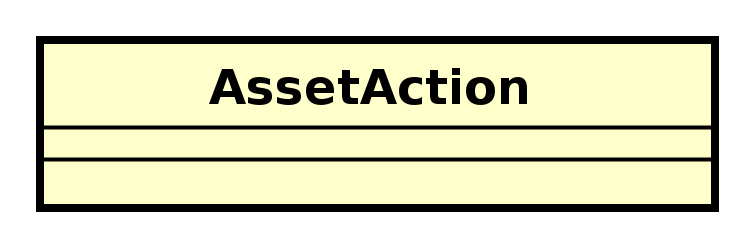
\includegraphics[width=0.3\textwidth]{./img/AssetAction.png}
		\caption{Diagramma classe AssetAction}
	\end{figure}
	\item \textbf{descrizione:} rappresenta un'azione relativa agli asset;
	\item \textbf{utilizzo:} l'azione viene creata da un apposito ActionCreator per essere poi inviata ad un reducer.
\end{itemize}
\paragraph{NodeAction}
\begin{itemize}
	\begin{figure}[H]
		\centering
		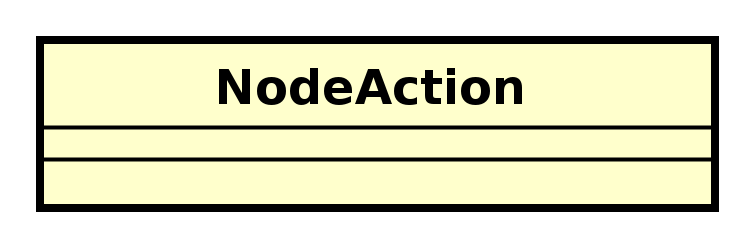
\includegraphics[width=0.3\textwidth]{./img/NodeAction.png}
		\caption{Diagramma classe NodeAction}
	\end{figure}
	\item \textbf{descrizione:} rappresenta un'azione relativa ai nodi;
	\item \textbf{utilizzo:} l'azione viene creata da un apposito ActionCreator per essere poi inviata ad un reducer.
\end{itemize}
\paragraph{OptionAction}
\begin{itemize}
	\begin{figure}[H]
		\centering
		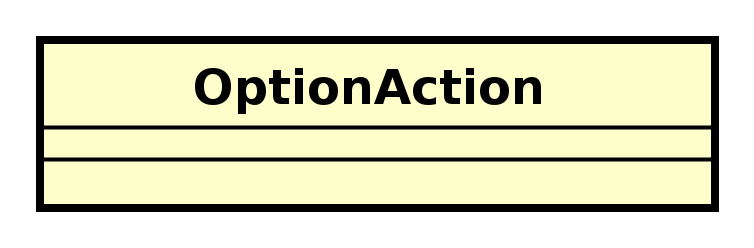
\includegraphics[width=0.3\textwidth]{./img/OptionAction.png}
		\caption{Diagramma classe OptionAction}
	\end{figure}
	\item \textbf{descrizione:} rappresenta un'azione relativa all'oggetto option;
	\item \textbf{utilizzo:} l'azione viene creata da un apposito ActionCreator per essere poi inviata ad un reducer;
	\item \textbf{relazioni con altre classi:} 
	\begin{itemize}
		\item IN OptionActionCreator.
	\end{itemize}
\end{itemize}
\newpage
\subsection{DeGeOP::ActionPkg::ActionCreatorsPkg}
\label{pkg::ActionCreatorsPkg}
\subsubsection{Informazioni sul package}
\begin{itemize}
	\item \textbf{descrizione:} racchiude le componenti che gestiscono la creazione delle azioni;
	\item \textbf{padre:} \hyperref[pkg::ActionPkg]{ActionPkg};
	\item \textbf{interazioni con altri package:} 
	\begin{itemize}
		\item OUT ActionElementsPkg: creazione di azioni.
	\end{itemize}
	\item \textbf{classi contenute:}
	\begin{itemize}
		\item AssetActionCreator;
		\item EdgeActionCreator;
		\item NodeActionCreator;
		\item OptionActionCreator.
	\end{itemize}
\end{itemize}
\subsubsection{Classi}
\paragraph{AssetActionCreator}
\begin{itemize}
	\begin{figure}[H]
		\centering
		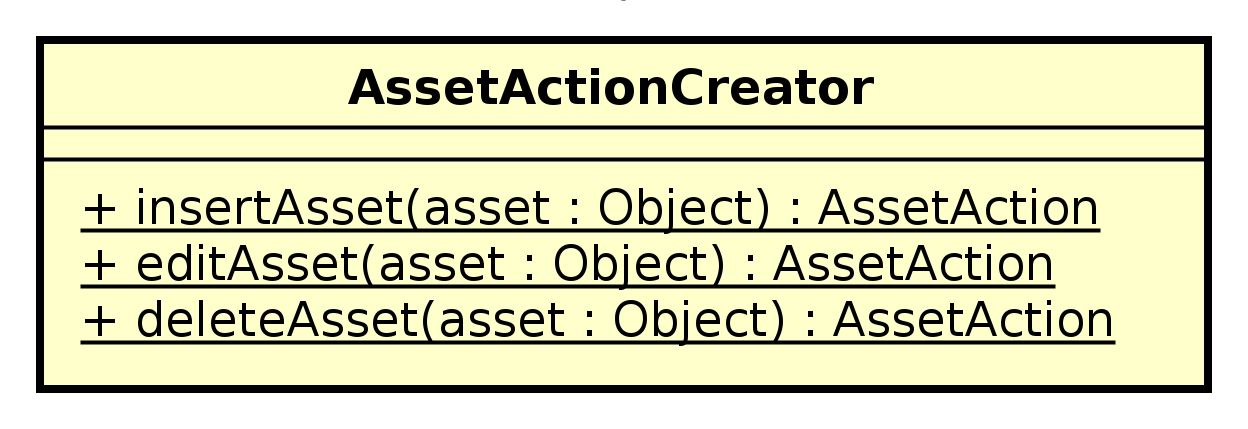
\includegraphics[width=0.3\textwidth]{./img/AssetActionCreator.png}
		\caption{Diagramma classe AssetActionCreator}
	\end{figure}
	\item \textbf{descrizione:} rappresenta la factory di azioni relative agli asset;
	\item \textbf{utilizzo:} i suoi metodi sono chiamati dalla View e dal CallManager per la creazione di azioni relative agli asset;
	\item \textbf{metodi:}
	\begin{itemize}
		\item +deleteAsset(asset) : AssetAction\newline
		il metodo crea l'azione relativa all'eliminazione dell'asset ricevuto in input
		\begin{itemize}
			\item asset : Object\\
			oggetto contenente i parametri di un Asset che dovrà essere eliminato.
		\end{itemize}
		\item +editAsset(asset) : AssetAction\newline
		il metodo crea l'azione relativa alla modifica di un asset
		\begin{itemize}
			\item asset : Object\\
			oggetto contenente i parametri di un Asset che dovrà essere modificato nello store.
		\end{itemize}
		\item +insertAsset(asset) : AssetAction\newline
		il metodo crea l'azione relativa all'inserimento di un nuovo asset
		\begin{itemize}
			\item asset : Object\\
			oggetto contenente i parametri di un Asset che dovrà essere inserito nello store.
		\end{itemize}
	\end{itemize}
\end{itemize}
\paragraph{EdgeActionCreator}
\begin{itemize}
	\begin{figure}[H]
		\centering
		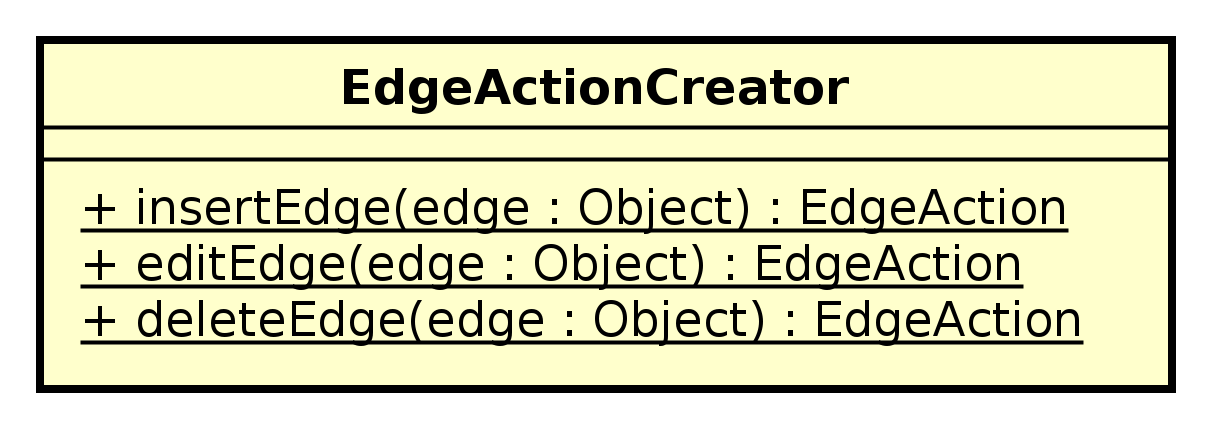
\includegraphics[width=0.3\textwidth]{./img/EdgeActionCreator.png}
		\caption{Diagramma classe EdgeActionCreator}
	\end{figure}
	\item \textbf{descrizione:} rappresenta la factory di azioni relative agli archi;
	\item \textbf{utilizzo:} i suoi metodi sono chiamati dalla View e dal CallManager per la creazione di azioni relative agli archi;
	\item \textbf{metodi:}
	\begin{itemize}
		\item +deleteEdge(edge) : EdgeAction\newline
		il metodo crea l'azione relativa all'eliminazione di un arco
		\begin{itemize}
			\item edge : Object\\
			oggetto contenente i parametri di un arco che dovrà essere eliminato.
		\end{itemize}
		\item +editEdge(edge) : EdgeAction\newline
		il metodo crea l'azione relativa alla modifica di un arco
		\begin{itemize}
			\item edge : Object\\
			oggetto contenente i parametri di un arco che dovrà essere modificato nello store.
		\end{itemize}
		\item +insertEdge(edge) : EdgeAction\newline
		il metodo crea l'azione relativa all'inserimento di un nuovo arco
		\begin{itemize}
			\item edge : Object\\
			oggetto contenente i parametri di un arco che dovrà essere inserito nello store.
		\end{itemize}
	\end{itemize}
\end{itemize}
\paragraph{NodeActionCreator}
\begin{itemize}
	\begin{figure}[H]
		\centering
		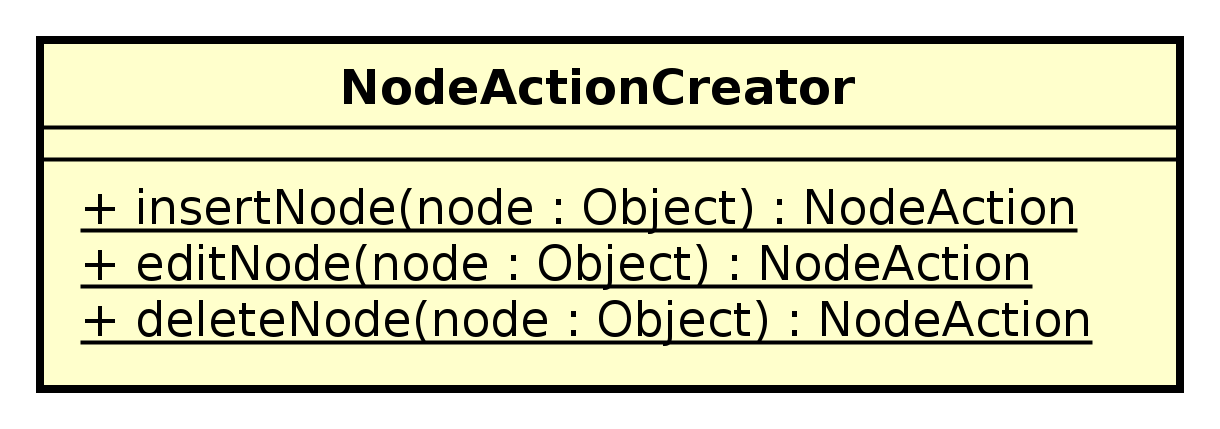
\includegraphics[width=0.3\textwidth]{./img/NodeActionCreator.png}
		\caption{Diagramma classe NodeActionCreator}
	\end{figure}
	\item \textbf{descrizione:} rappresenta la factory di azioni relative ai nodi;
	\item \textbf{utilizzo:} i suoi metodi sono chiamati dalla View e dal CallManager per la creazione di azioni relative ai nodi;
	\item \textbf{metodi:}
	\begin{itemize}
		\item +deleteNode(node) : NodeAction\newline
		il metodo crea l'azione relativa all'eliminazione di un nodo
		\begin{itemize}
			\item node : Object\\
			oggetto contenente i parametri di un nodo che dovrà essere eliminato.
		\end{itemize}
		\item +editNode(node) : NodeAction\newline
		il metodo crea l'azione relativa alla modifica di un nodo
		\begin{itemize}
			\item node : Object\\
			oggetto contenente i parametri di un nodo che dovrà essere modificato nello store.
		\end{itemize}
		\item +insertNode(node) : NodeAction\newline
		il metodo crea l'azione relativa all'inserimento di un nuovo nodo
		\begin{itemize}
			\item node : Object\\
			oggetto contenente i parametri di un nodo che dovrà essere inserito nello store.
		\end{itemize}
	\end{itemize}
\end{itemize}
\paragraph{OptionActionCreator}
\begin{itemize}
	\begin{figure}[H]
		\centering
		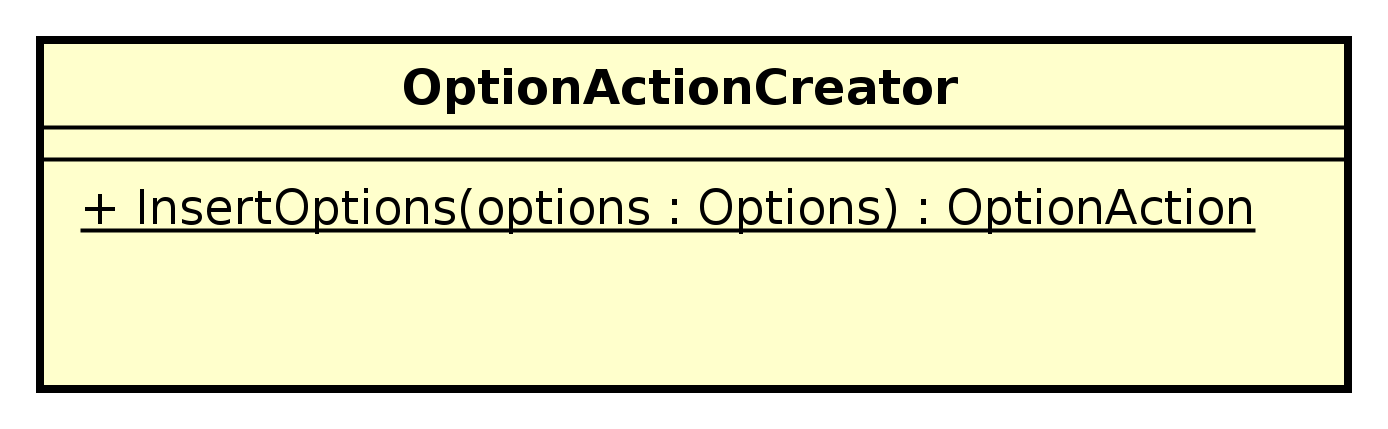
\includegraphics[width=0.3\textwidth]{./img/OptionActionCreator.png}
		\caption{Diagramma classe OptionActionCreator}
	\end{figure}
	\item \textbf{descrizione:} rappresenta la factory di azioni relative agli asset;
	\item \textbf{utilizzo:} i suoi metodi sono chiamati dalla View e dal CallManager per la creazione di azioni relative agli asset;
	\item \textbf{metodi:}
	\begin{itemize}
		\item +insertOptions() : OptionAction\newline
		il metodo crea l'azione relativa all'inserimento dell'oggetto options dello store
	\end{itemize}
	\item \textbf{relazioni con altre classi:} 
	\begin{itemize}
		\item OUT OptionAction.
	\end{itemize}
\end{itemize}
\newpage
\subsection{DeGeOP::ViewPkg}
\label{pkg::ViewPkg}
\begin{figure}[H]
	\centering
	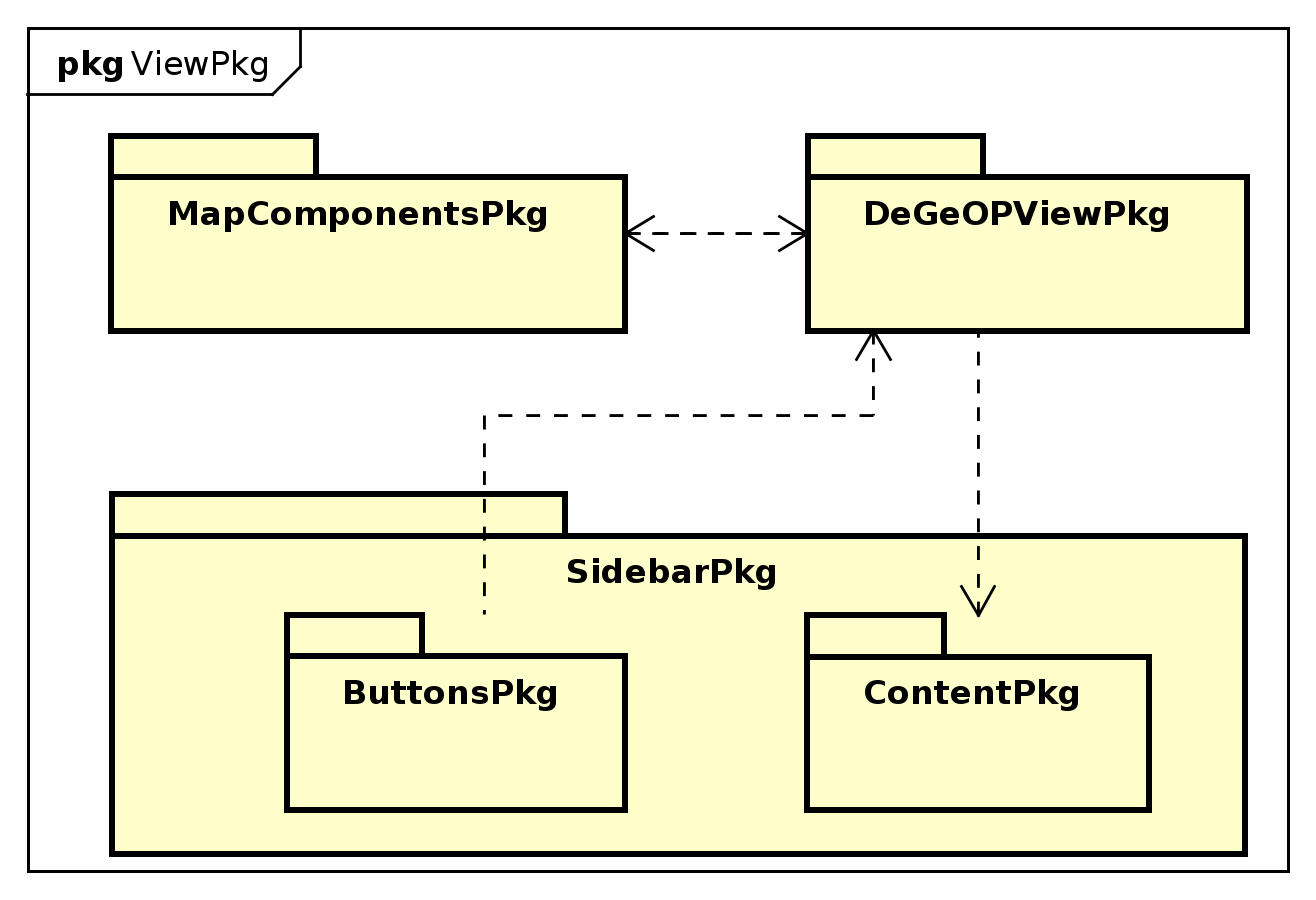
\includegraphics[width=\textwidth]{img/PkgDiagram/ViewPkg.png}
	\caption{Schema componente DeGeOP::ViewPkg}
\end{figure}
\subsubsection{Informazioni sul package}
\begin{itemize}
	\item \textbf{descrizione:} racchiude le componenti per la visualizzazione dell'interfaccia utente;
	\item \textbf{padre:} \hyperref[pkg::DeGeOP]{DeGeOP};
	\item \textbf{package contenuti:}
	\begin{itemize}
		\item ViewPkg::\hyperref[pkg::DeGeOPViewPkg]{DeGeOPViewPkg};
		\item ViewPkg::\hyperref[pkg::MapComponentsPkg]{MapComponentsPkg};
		\item ViewPkg::\hyperref[pkg::SidebarPkg]{SidebarPkg}.
	\end{itemize}
	\item \textbf{interazioni con altri package:} 
	\begin{itemize}
		\item OUT ActionPkg: dispatch di azioni;
		\item OUT Alexa voice service: gestore vocale;
		\item OUT Hammer: gestione gesture ;
		\item OUT Openlayers: gestione mappa;
		\item OUT React: utilizzo componenti react;
		\item OUT ReactToolbox: utilizzo componenti material design;
		\item OUT Redux: utilizzo metodo dispatch;
		\item OUT StorePkg: subscribe sullo store.
	\end{itemize}
\end{itemize}
\newpage
\subsection{DeGeOP::ViewPkg::DeGeOPViewPkg}
\label{pkg::DeGeOPViewPkg}
\begin{figure}[H]
	\centering
	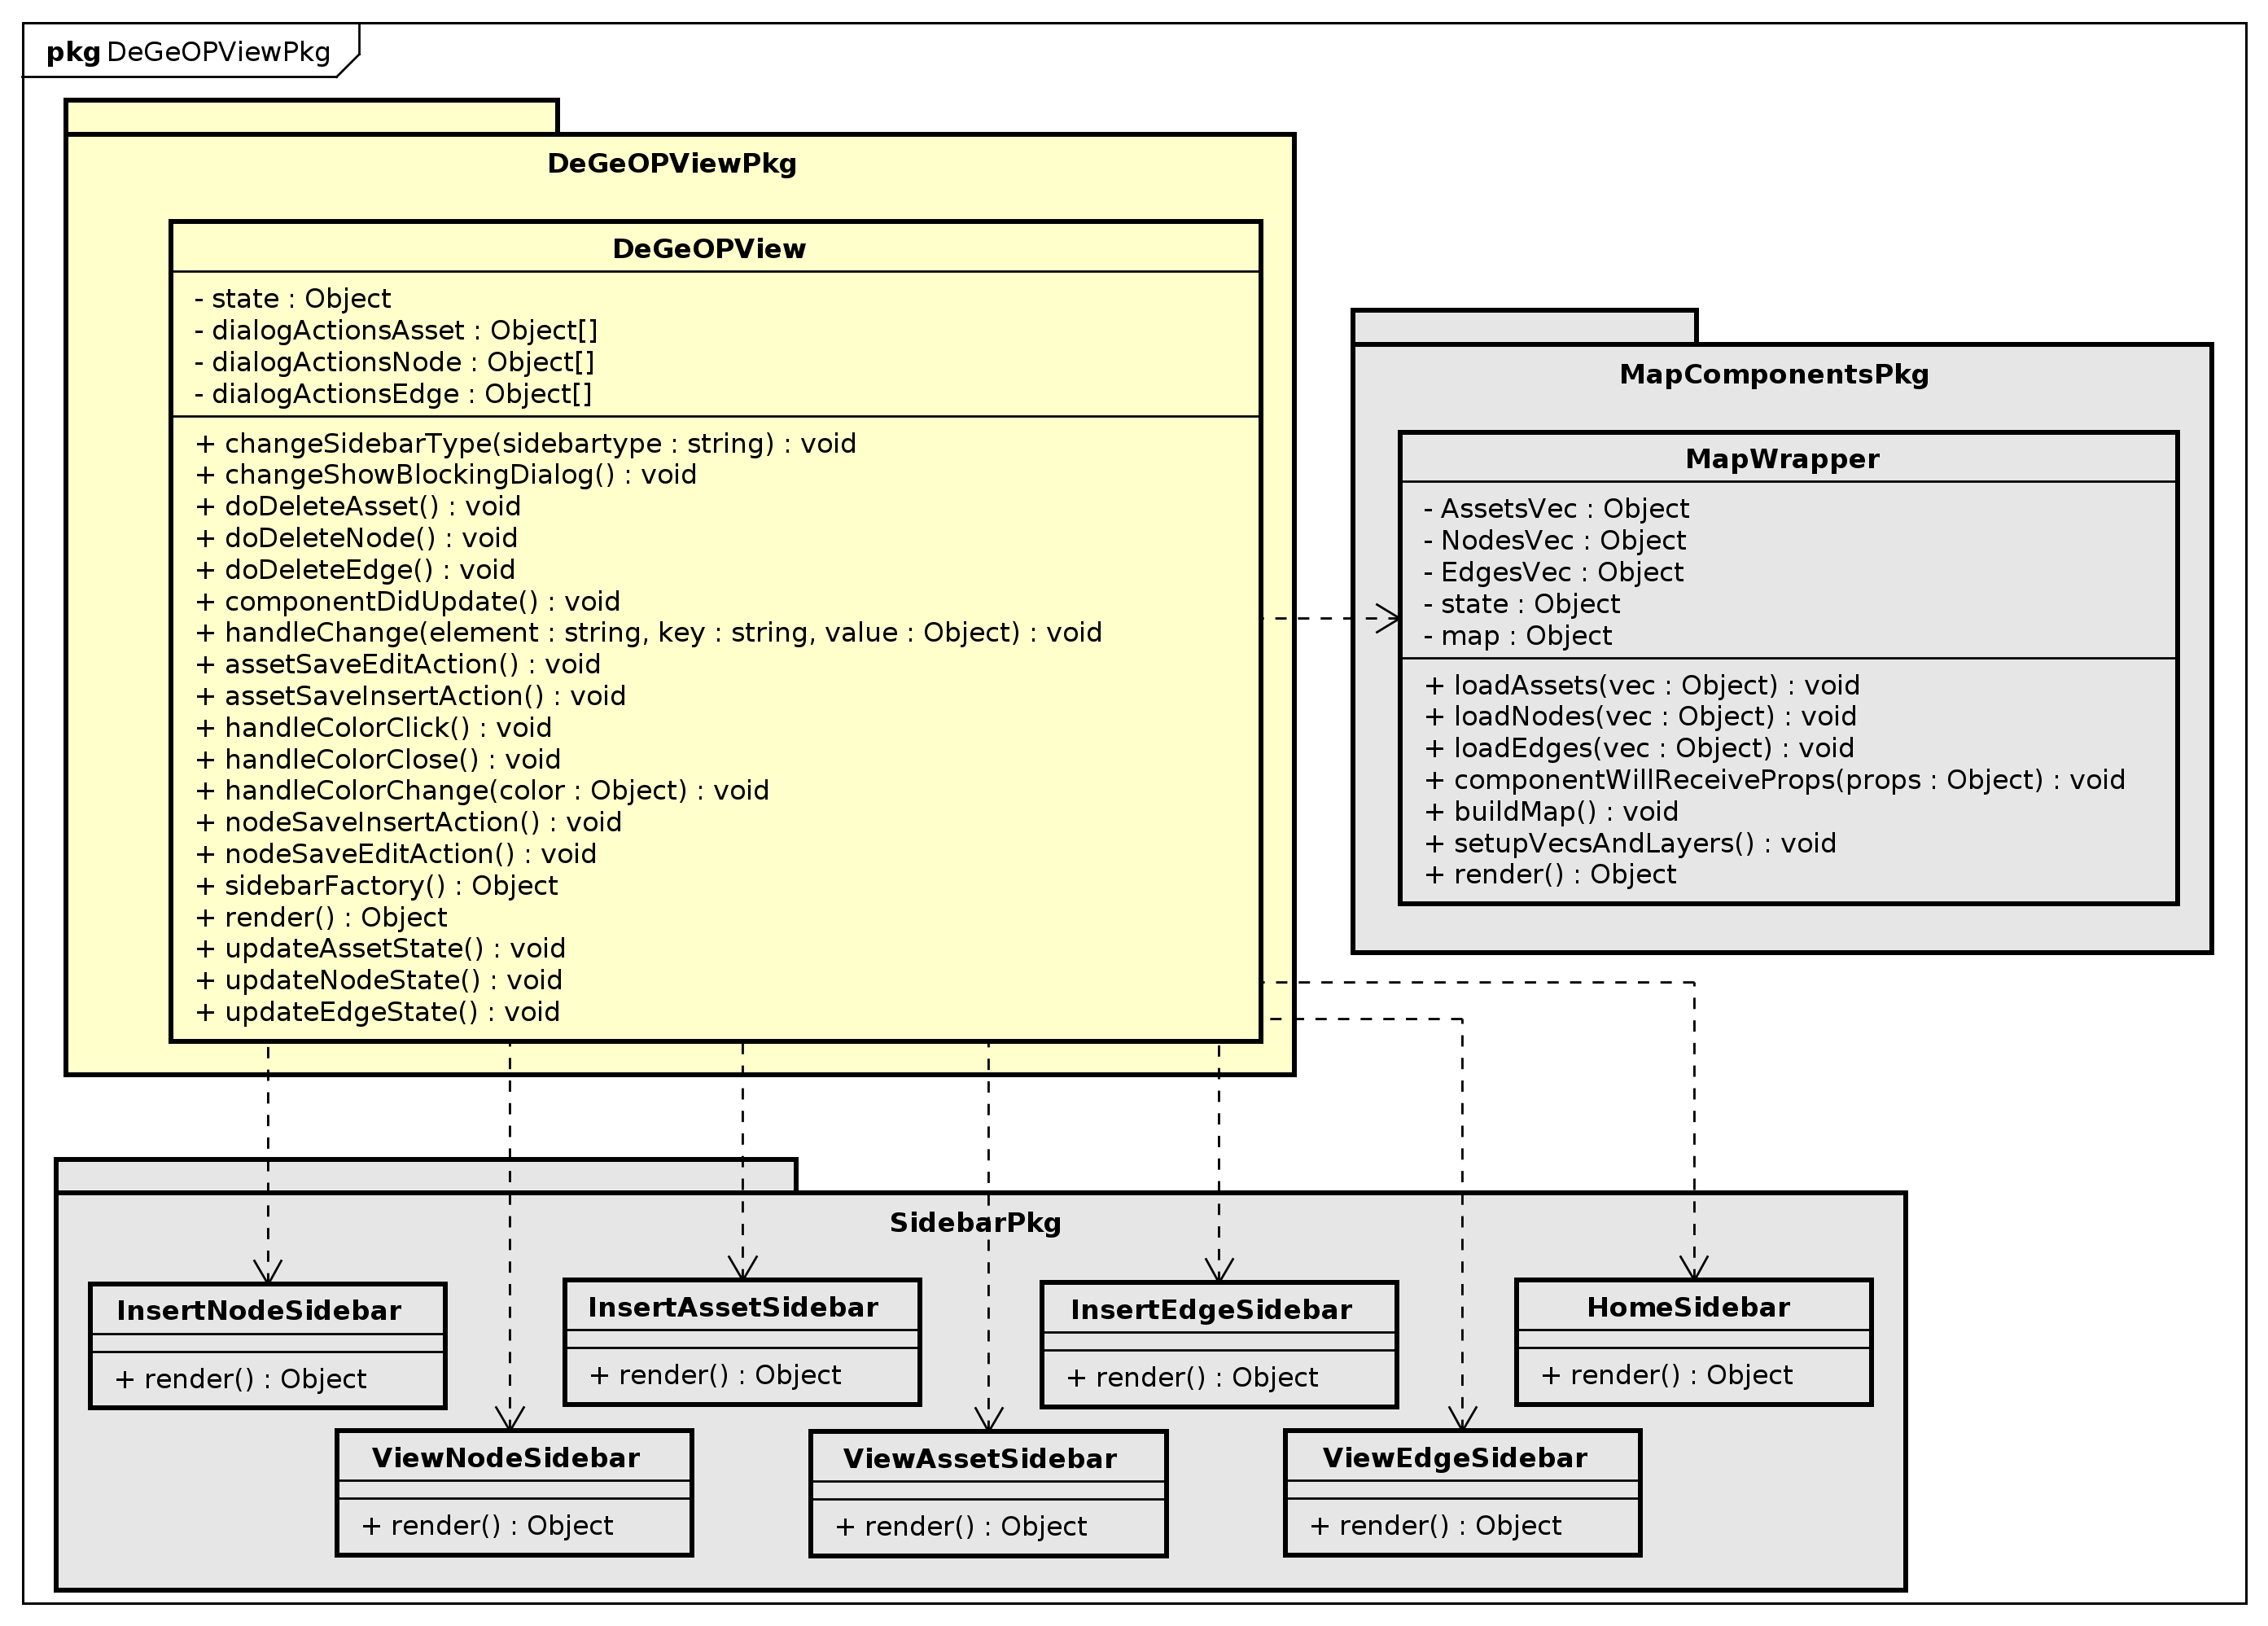
\includegraphics[width=\textwidth]{img/PkgDiagram/DeGeOPViewPkg.png}
	\caption{Schema componente DeGeOP::ViewPkg::DeGeOPViewPkg}
\end{figure}
\subsubsection{Informazioni sul package}
\begin{itemize}
	\item \textbf{descrizione:} racchiude la componente principale della view;
	\item \textbf{padre:} \hyperref[pkg::ViewPkg]{ViewPkg};
	\item \textbf{interazioni con altri package:} 
	\begin{itemize}
		\item IN MapComponentsPkg: utilizzo di componenti grafiche;
		\item OUT MapComponentsPkg: utilizzo di componenti grafiche;
		\item OUT SidebarPkg: utilizzo della sidebar.
	\end{itemize}
	\item \textbf{classi contenute:}
	\begin{itemize}
		\item DeGeOPView.
	\end{itemize}
\end{itemize}
\subsubsection{Classi}
\paragraph{DeGeOPView}
\begin{itemize}
	\begin{figure}[H]
		\centering
		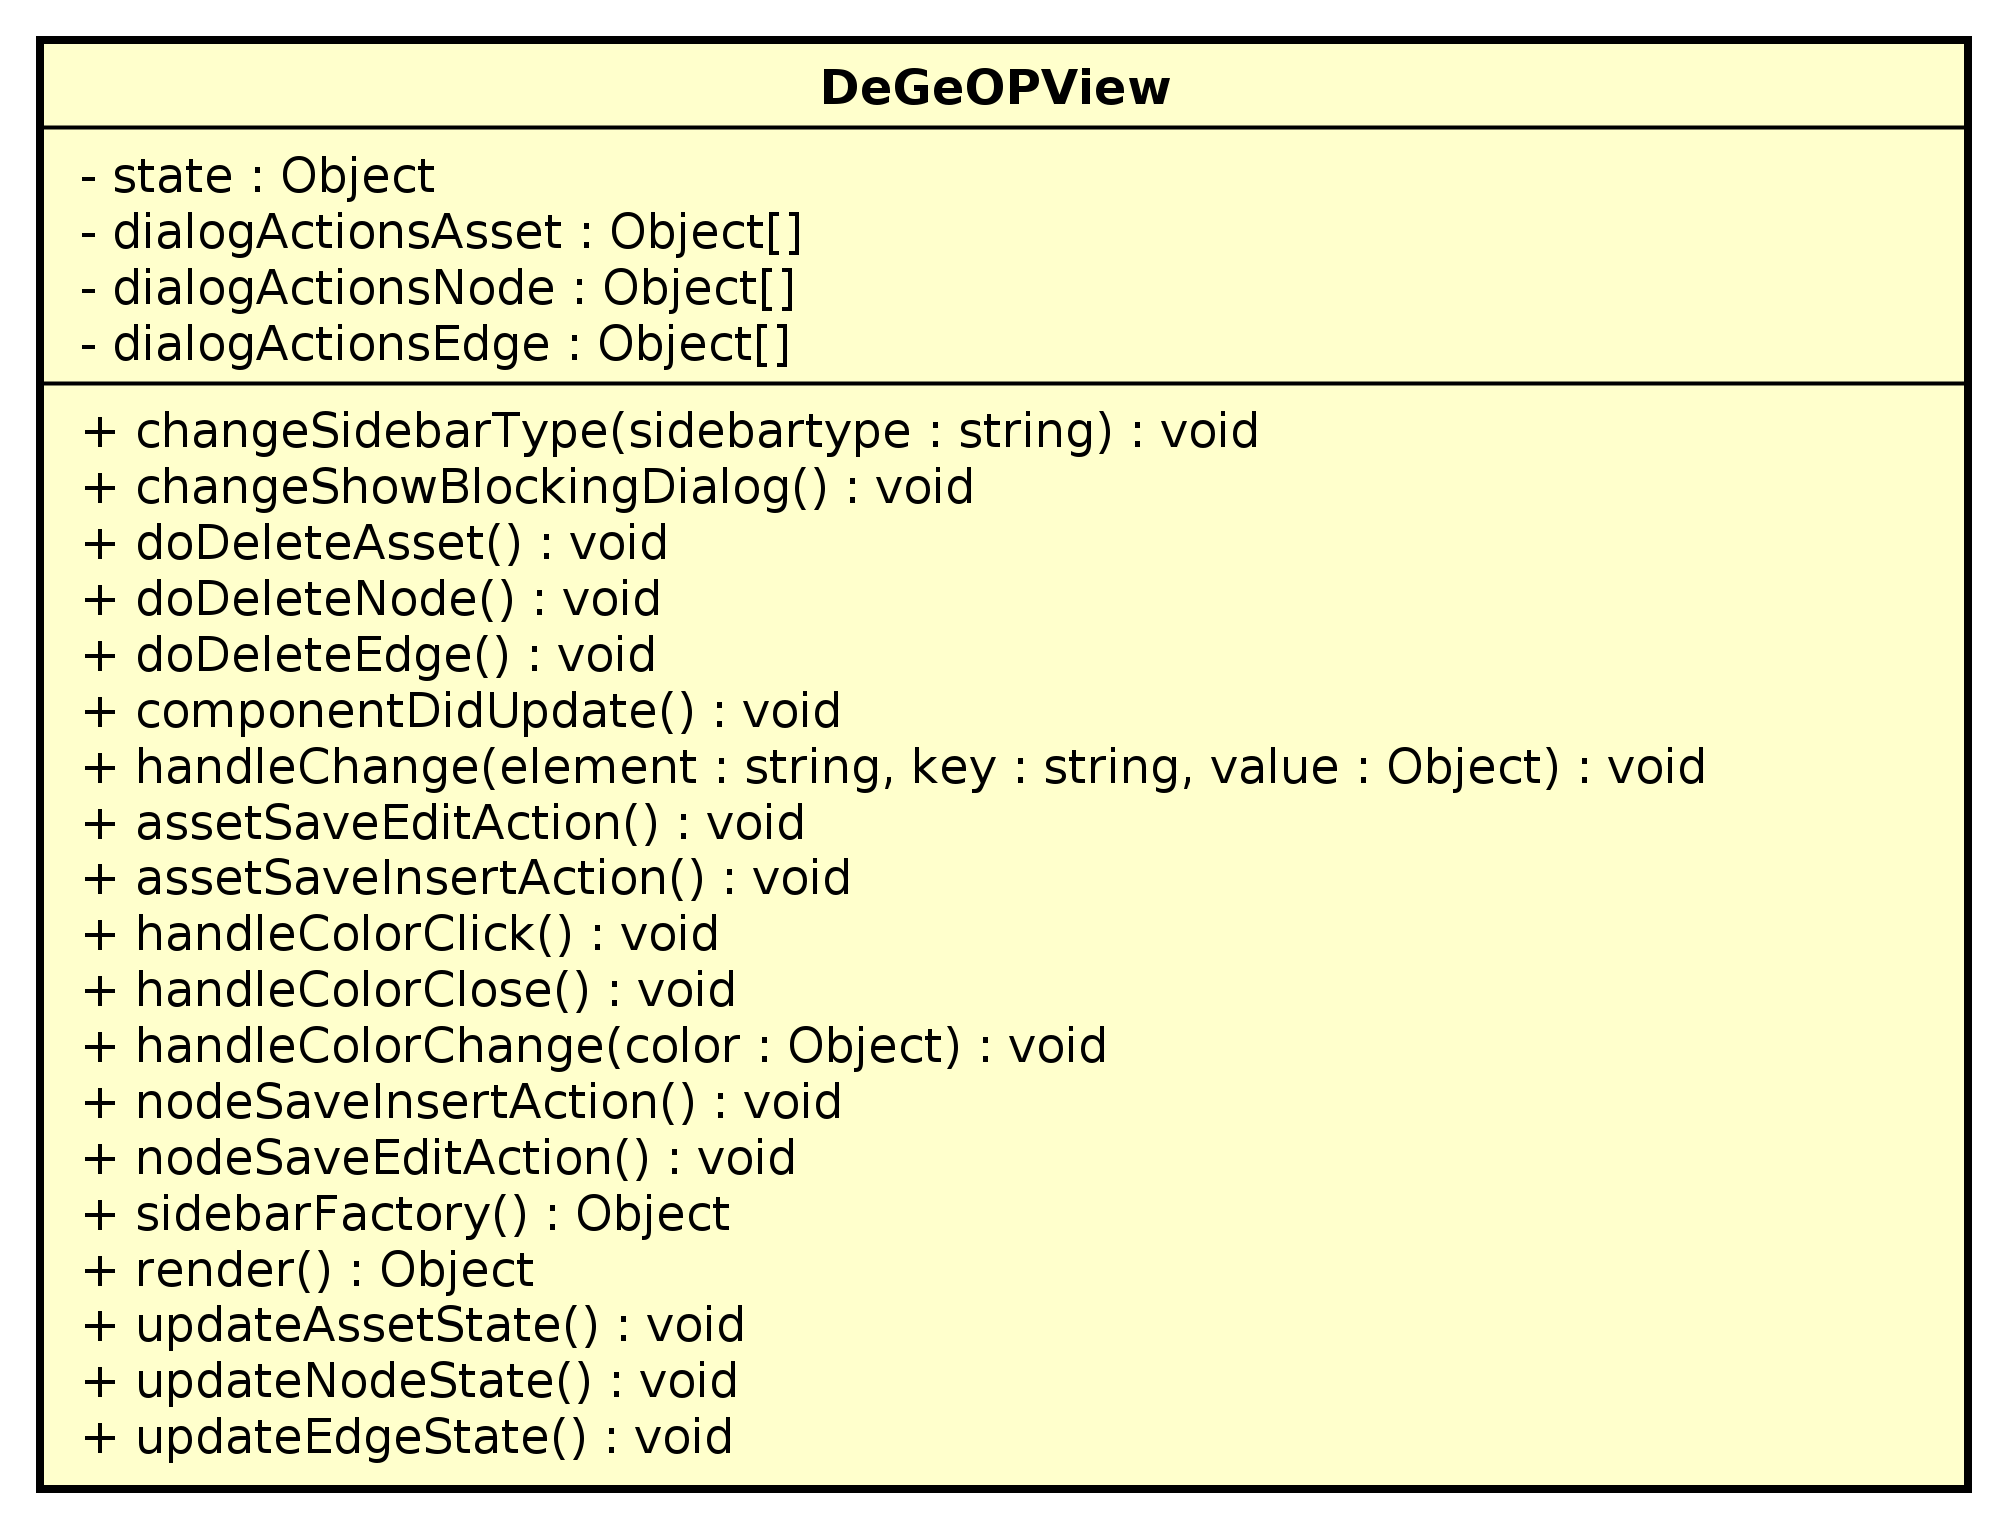
\includegraphics[width=0.3\textwidth]{./img/DeGeOPView.png}
		\caption{Diagramma classe DeGeOPView}
	\end{figure}
	\item \textbf{descrizione:} rappresenta l'oggetto grafico radice, che comprende l'intera View del prodotto;
	\item \textbf{utilizzo:} i suoi metodi setter sono richiamati da ConcreteDeGeOPViewBuilder per impostare i suoi campi dati. La classe effettua il subscribe sullo Store per ricevere gli aggiornamenti ;
	\item \textbf{attributi:}
	\begin{itemize}
		\item -dialogActionsAsset : Object[]\begin{itemize}
			\item contiene le funzioni richiamate durante la visualizzazione della schermata modale relativa agli asset.\end{itemize}
		\item -dialogActionsEdge : Object[]\begin{itemize}
			\item contiene le funzioni richiamate durante la visualizzazione della schermata modale relativa ai nodi.\end{itemize}
		\item -dialogActionsNode : Object[]\begin{itemize}
			\item contiene le funzioni richiamate durante la visualizzazione della schermata modale relativa ai nodi.\end{itemize}
		\item -state : Object\begin{itemize}
			\item rappresenta lo stato di DeGeOPView, ovvero i dati temporanei che l'utente inserisce prima che vengano inseriti nello store.\end{itemize}
	\end{itemize}
	\item \textbf{metodi:}
	\begin{itemize}
		\item +assetSaveEditAction() : void\newline
		il metodo emette l'azione relativa alla modifica di un asset
		\item +assetSaveInsertAction() : void\newline
		il metodo emette l'azione relativa all'inserimento di un asset
		\item +changeShowBlockingDialog() : void\newline
		il metodo gestisce il cambiamento del booleano nello state di DeGeOPView che gestisce la visualizzazione della finestra modale
		\item +changeSidebarType() : void\newline
		il metodo gestisce il cambiamento della stringa dello state di DeGeOPView che gestisce il tipo di sidebar visualizzata al momento
		\item +componentDidUpdate() : void\newline
		il metodo viene richiamato quando lo state di DeGeOPView cambia; al suo interno vengono gestite le validazioni dei campi compilati dall'utente
		\item +doDeleteAsset() : void\newline
		il metodo emette l'azione di eliminazione dell'asset attualmente selezionato e ne fa il dispatch verso lo store
		\item +doDeleteEdge() : void\newline
		il metodo emette l'azione di eliminazione del nodo attualmente selezionato e ne fa il dispatch verso lo store
		\item +doDeleteNode() : void\newline
		il metodo emette l'azione di eliminazione del nodo attualmente selezionato e ne fa il dispatch verso lo store
		\item +handleChange(element, key, value) : void\newline
		il metodo gestisce il cambiamento di stato di DeGeOPView relativamente ai campi dati compilati dall'utente
		\begin{itemize}
			\item element : string\\
			indica il campo dati dello stato di DeGeOPView da cambiare. Può assumere i valori:
			asset, node, edge, common.
			\item key : string\\
			indica il campo dati dell'oggetto descritto da element che dovrà essere modificato.
			\item value : Object\\
			indica il valore da inserire nell'oggetto descritto da element, nel campo dati descritto da key.
		\end{itemize}
		\item +handleColorChange(color) : void\newline
		il metodo gestisce il cambiamento nello state di DeGeOPView relativo al colore selezionato dalla palette colori
		\begin{itemize}
			\item color : Object\\
			rappresenta il nuovo colore selezionato dalla palette colori.
		\end{itemize}
		\item +handleColorClick() : void\newline
		il metodo gestisce l'apertura e la chiusura della palette colori
		\item +handleColorClose() : void\newline
		il metodo gestisce la chiusura della palette colori
		\item +nodeSaveEditAction() : void\newline
		il metodo gestisce l'emissione dell'azione relativa alla modifica di un nodo
		\item +nodeSaveInsertAction() : void\newline
		il metodo gestisce l'emissione dell'azione relativa all'inserimento di un nodo
		\item +render() : Object\newline
		il metodo gestisce il render di DeGeOPView, composta da una sidebar e da un MapWrapper
		\item +sidebarFactory() : Object\newline
		il metodo gestisce la creazione di una sidebar da renderizzare in base alla stringa attualmente specificata nello state di DeGeOPView
		\item +updateAssetState() : void\newline
		il metodo imposta lo stato dell'asset in DeGeOPView con i dati dell'asset selezionato sulla mappa
		\item +updateEdgeState() : void\newline
		il metodo imposta lo stato dell'arco in DeGeOPView con i dati dell'arco selezionato sulla mappa
		\item +updateNodeState() : void\newline
		il metodo imposta lo stato del nodo in DeGeOPView con i dati del nodo selezionato sulla mappa
	\end{itemize}
\end{itemize}
\newpage
\subsection{DeGeOP::ViewPkg::MapComponentsPkg}
\label{pkg::MapComponentsPkg}
\begin{figure}[H]
	\centering
	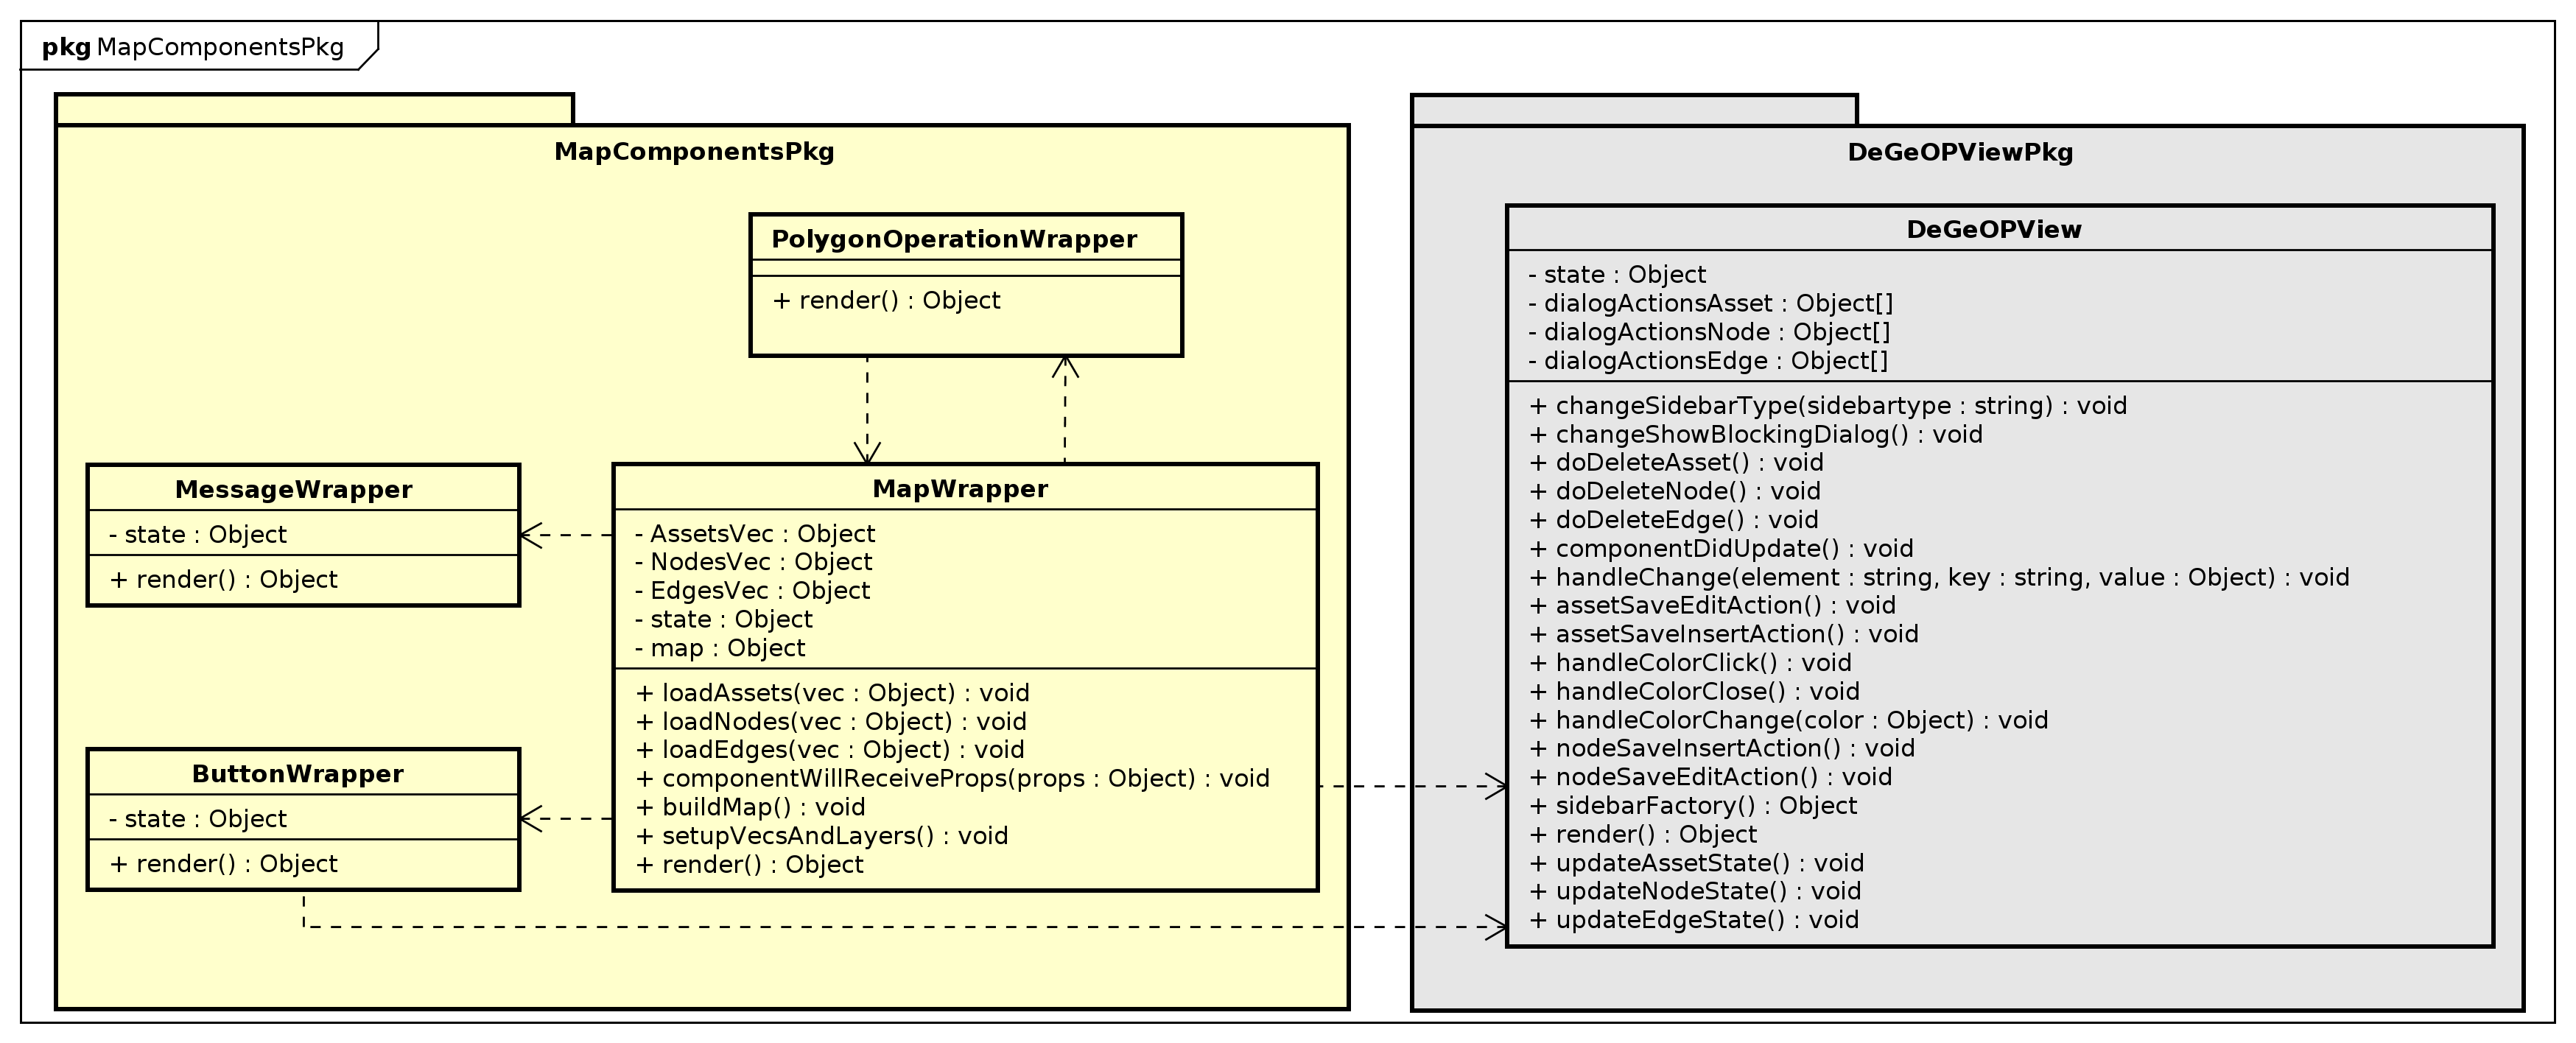
\includegraphics[width=\textwidth]{img/PkgDiagram/MapComponentsPkg.png}
	\caption{Schema componente DeGeOP::ViewPkg::MapComponentsPkg}
\end{figure}
\subsubsection{Informazioni sul package}
\begin{itemize}
	\item \textbf{descrizione:} racchiude le componenti relative alla mappa e ai pulsanti sopra di essa;
	\item \textbf{padre:} \hyperref[pkg::ViewPkg]{ViewPkg};
	\item \textbf{interazioni con altri package:} 
	\begin{itemize}
		\item IN DeGeOPViewPkg: utilizzo di componenti grafiche;
		\item OUT DeGeOPViewPkg: utilizzo di componenti grafiche;
		\item OUT Openlayers: gestione mappa.
	\end{itemize}
	\item \textbf{classi contenute:}
	\begin{itemize}
		\item ButtonWrapper;
		\item MapWrapper;
		\item MessageWrapper;
		\item PolygonOperationWrapper.
	\end{itemize}
\end{itemize}
\subsubsection{Classi}
\paragraph{ButtonWrapper}
\begin{itemize}
	\begin{figure}[H]
		\centering
		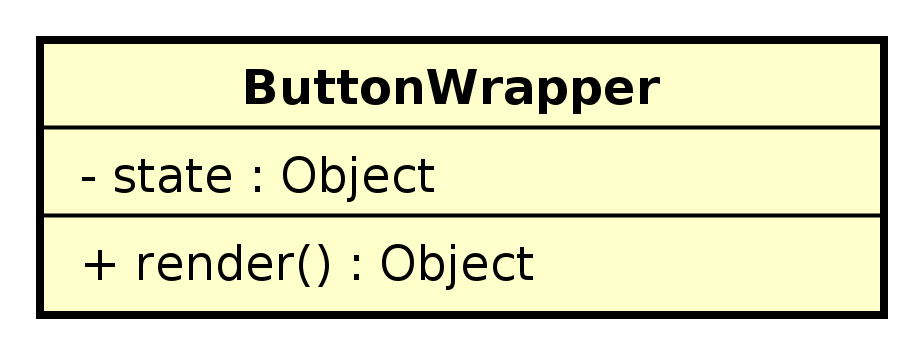
\includegraphics[width=0.3\textwidth]{./img/ButtonWrapper.png}
		\caption{Diagramma classe ButtonWrapper}
	\end{figure}
	\item \textbf{descrizione:} rappresenta una classe wrapper per visualizzare una serie di bottoni con cui è possibile eseguire varie operazioni;
	\item \textbf{utilizzo:} viene utilizzato per mostrare sulla mappa una serie di bottoni;
	\item \textbf{attributi:}
	\begin{itemize}
		\item -state : Object\begin{itemize}
			\item rappresenta lo stato del ButtonWrapper.\end{itemize}
	\end{itemize}
	\item \textbf{relazioni con altre classi:} 
	\begin{itemize}
		\item IN MapWrapper.
	\end{itemize}
\end{itemize}
\paragraph{MapWrapper}
\begin{itemize}
	\begin{figure}[H]
		\centering
		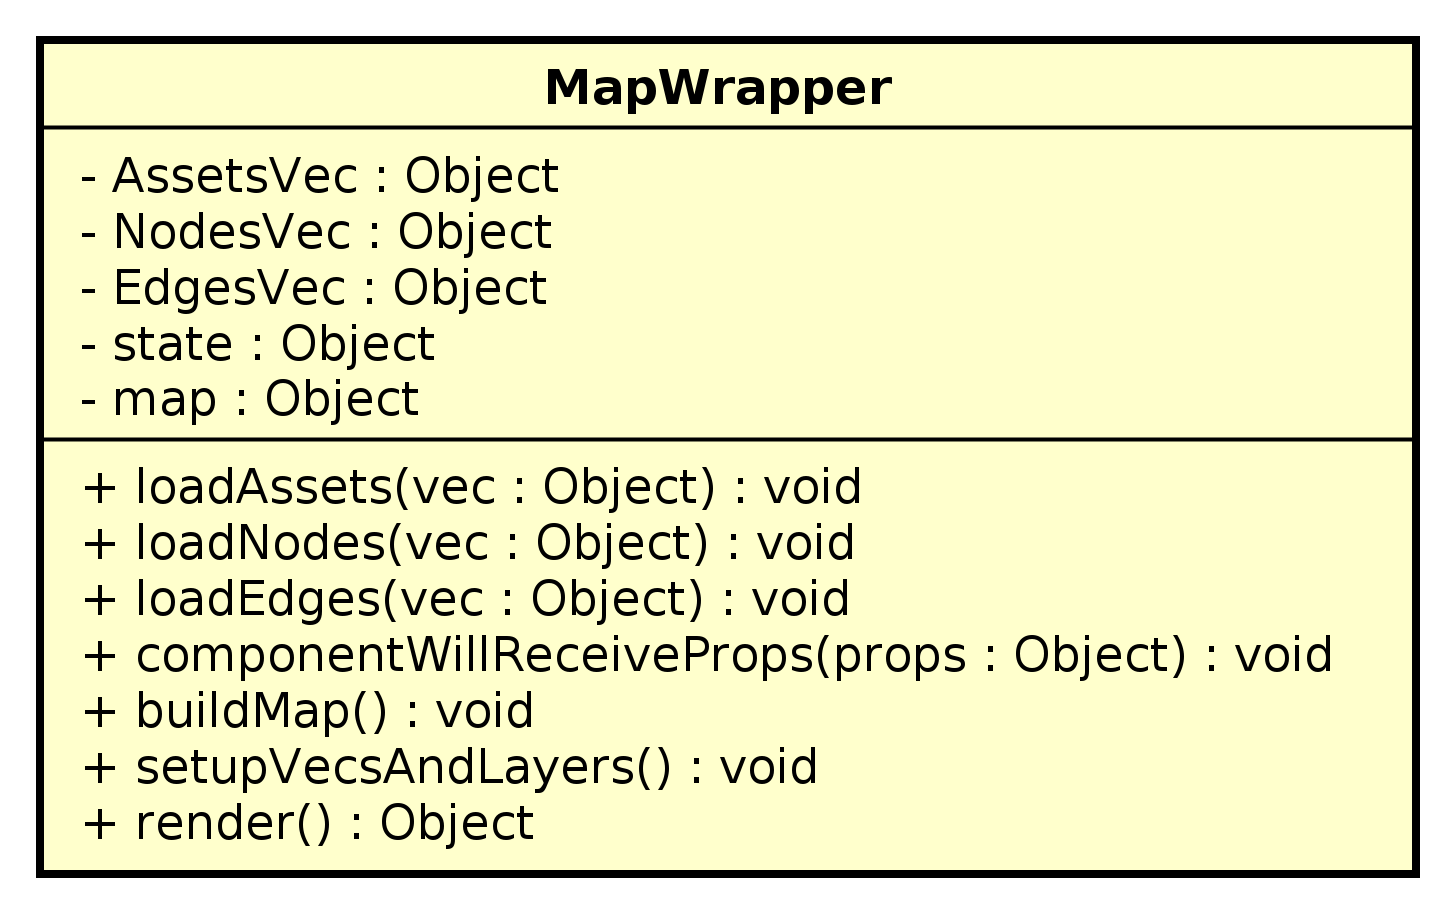
\includegraphics[width=0.3\textwidth]{./img/MapWrapper.png}
		\caption{Diagramma classe MapWrapper}
	\end{figure}
	\item \textbf{descrizione:} rappresenta una classe wrapper per visualizzare la mappa;
	\item \textbf{utilizzo:} viene utilizzata per visualizzare una mappa e permettere all'utente di interagire con essa;
	\item \textbf{attributi:}
	\begin{itemize}
		\item -assetsVec : Object\begin{itemize}
			\item contiene gli oggetti geometrici relativi agli asset da disegnare sulla mappa.\end{itemize}
		\item -edgesVec : Object\begin{itemize}
			\item contiene gli oggetti geometrici relativi agli asset da disegnare sulla mappa.\end{itemize}
		\item -map : Object\begin{itemize}
			\item oggetto che contiene lo stato della mappa.\end{itemize}
		\item -nodesVec : Object\begin{itemize}
			\item contiene gli oggetti geometrici relativi ai nodi da disegnare sulla mappa.\end{itemize}
		\item -state : Object\begin{itemize}
			\item contiene lo stato della classe MapWrapper.\end{itemize}
	\end{itemize}
	\item \textbf{metodi:}
	\begin{itemize}
		\item +buildMap() : void\newline
		il metodo costruisce la mappa
		\item +componentWillReceiveProps(props) : void\newline
		il metodo viene richiamato quando la componente MapWrapper sta per ricevere nuovi props
		\begin{itemize}
			\item props : Object\\
			props da ricevere.
		\end{itemize}
		\item +loadAssets(vec) : void\newline
		il metodo carica il vettore degli asset
		\begin{itemize}
			\item vec : Object\\
			vettore degli asset da caricare.
		\end{itemize}
		\item +loadEdges(vec) : void\newline
		il metodo carica il vettore degli archi
		\begin{itemize}
			\item vec : Object\\
			vettore degli archi da caricare.
		\end{itemize}
		\item +loadNodes(vec) : void\newline
		il metodo carica il vettore dei nodi
		\begin{itemize}
			\item vec : Object\\
			vettore dei nodi da caricare.
		\end{itemize}
		\item +render() : Object\newline
		renderizza il MapWrapper
		\item +setupVecsAndLayers() : void\newline
		il metodo prepara i vettori e i layers per la mappa
	\end{itemize}
	\item \textbf{relazioni con altre classi:} 
	\begin{itemize}
		\item IN PolygonOperationWrapper;
		\item OUT ButtonWrapper;
		\item OUT MessageWrapper;
		\item OUT PolygonOperationWrapper.
	\end{itemize}
\end{itemize}
\paragraph{MessageWrapper}
\begin{itemize}
	\begin{figure}[H]
		\centering
		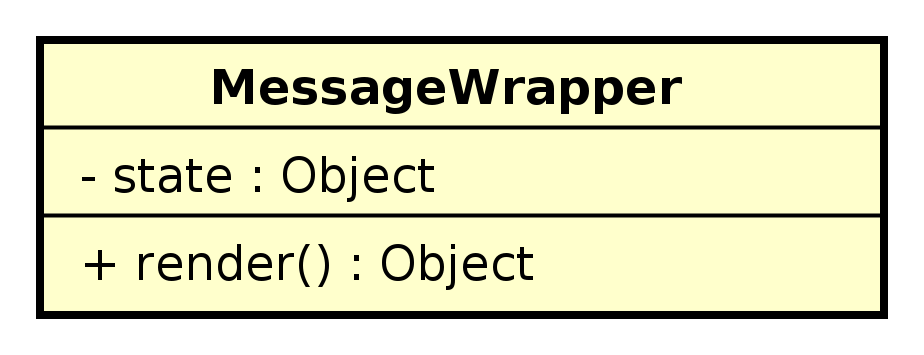
\includegraphics[width=0.3\textwidth]{./img/MessageWrapper.png}
		\caption{Diagramma classe MessageWrapper}
	\end{figure}
	\item \textbf{descrizione:} rappresenta una classe wrapper per visualizzare un messaggio;
	\item \textbf{utilizzo:} viene utilizzato per mostrare messaggi di errore o di successo sulla mappa;
	\item \textbf{attributi:}
	\begin{itemize}
		\item -state : Object\begin{itemize}
			\item rappresenta lo stato del MessageWrapper.\end{itemize}
	\end{itemize}
	\item \textbf{metodi:}
	\begin{itemize}
		\item +render() : Object\newline
		renderizza il MessageWrapper
	\end{itemize}
	\item \textbf{relazioni con altre classi:} 
	\begin{itemize}
		\item IN MapWrapper.
	\end{itemize}
\end{itemize}
\paragraph{PolygonOperationWrapper}
\begin{itemize}
	\begin{figure}[H]
		\centering
		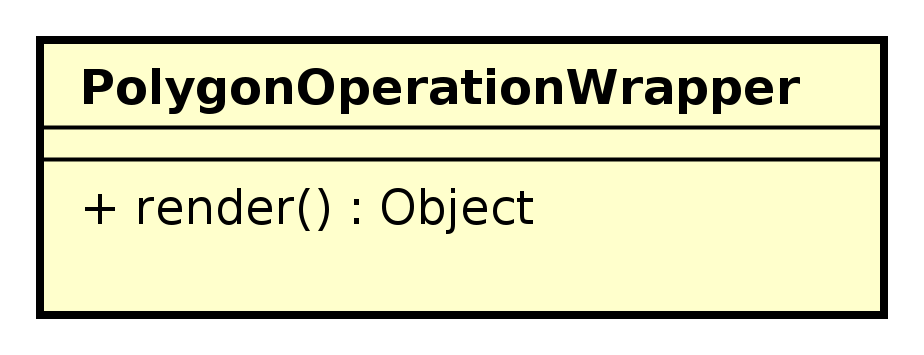
\includegraphics[width=0.3\textwidth]{./img/PolygonOperationWrapper.png}
		\caption{Diagramma classe PolygonOperationWrapper}
	\end{figure}
	\item \textbf{descrizione:} rappresenta una classe wrapper per visualizzare un bottone con cui è possibile effettuare operazioni sul perimetro di un poligono sulla mappa;
	\item \textbf{utilizzo:} invocando i suoi metodi è possibile iniziare a disegnare il poligono su mappa oppure cancellare l'ultimo segmento disegnato;
	\item \textbf{metodi:}
	\begin{itemize}
		\item +render() : Object\newline
		renderizza il PolygonOperationWrapper
	\end{itemize}
	\item \textbf{relazioni con altre classi:} 
	\begin{itemize}
		\item IN MapWrapper;
		\item OUT MapWrapper.
	\end{itemize}
\end{itemize}
\newpage
\subsection{DeGeOP::ViewPkg::SidebarPkg}
\label{pkg::SidebarPkg}
\begin{figure}[H]
	\centering
	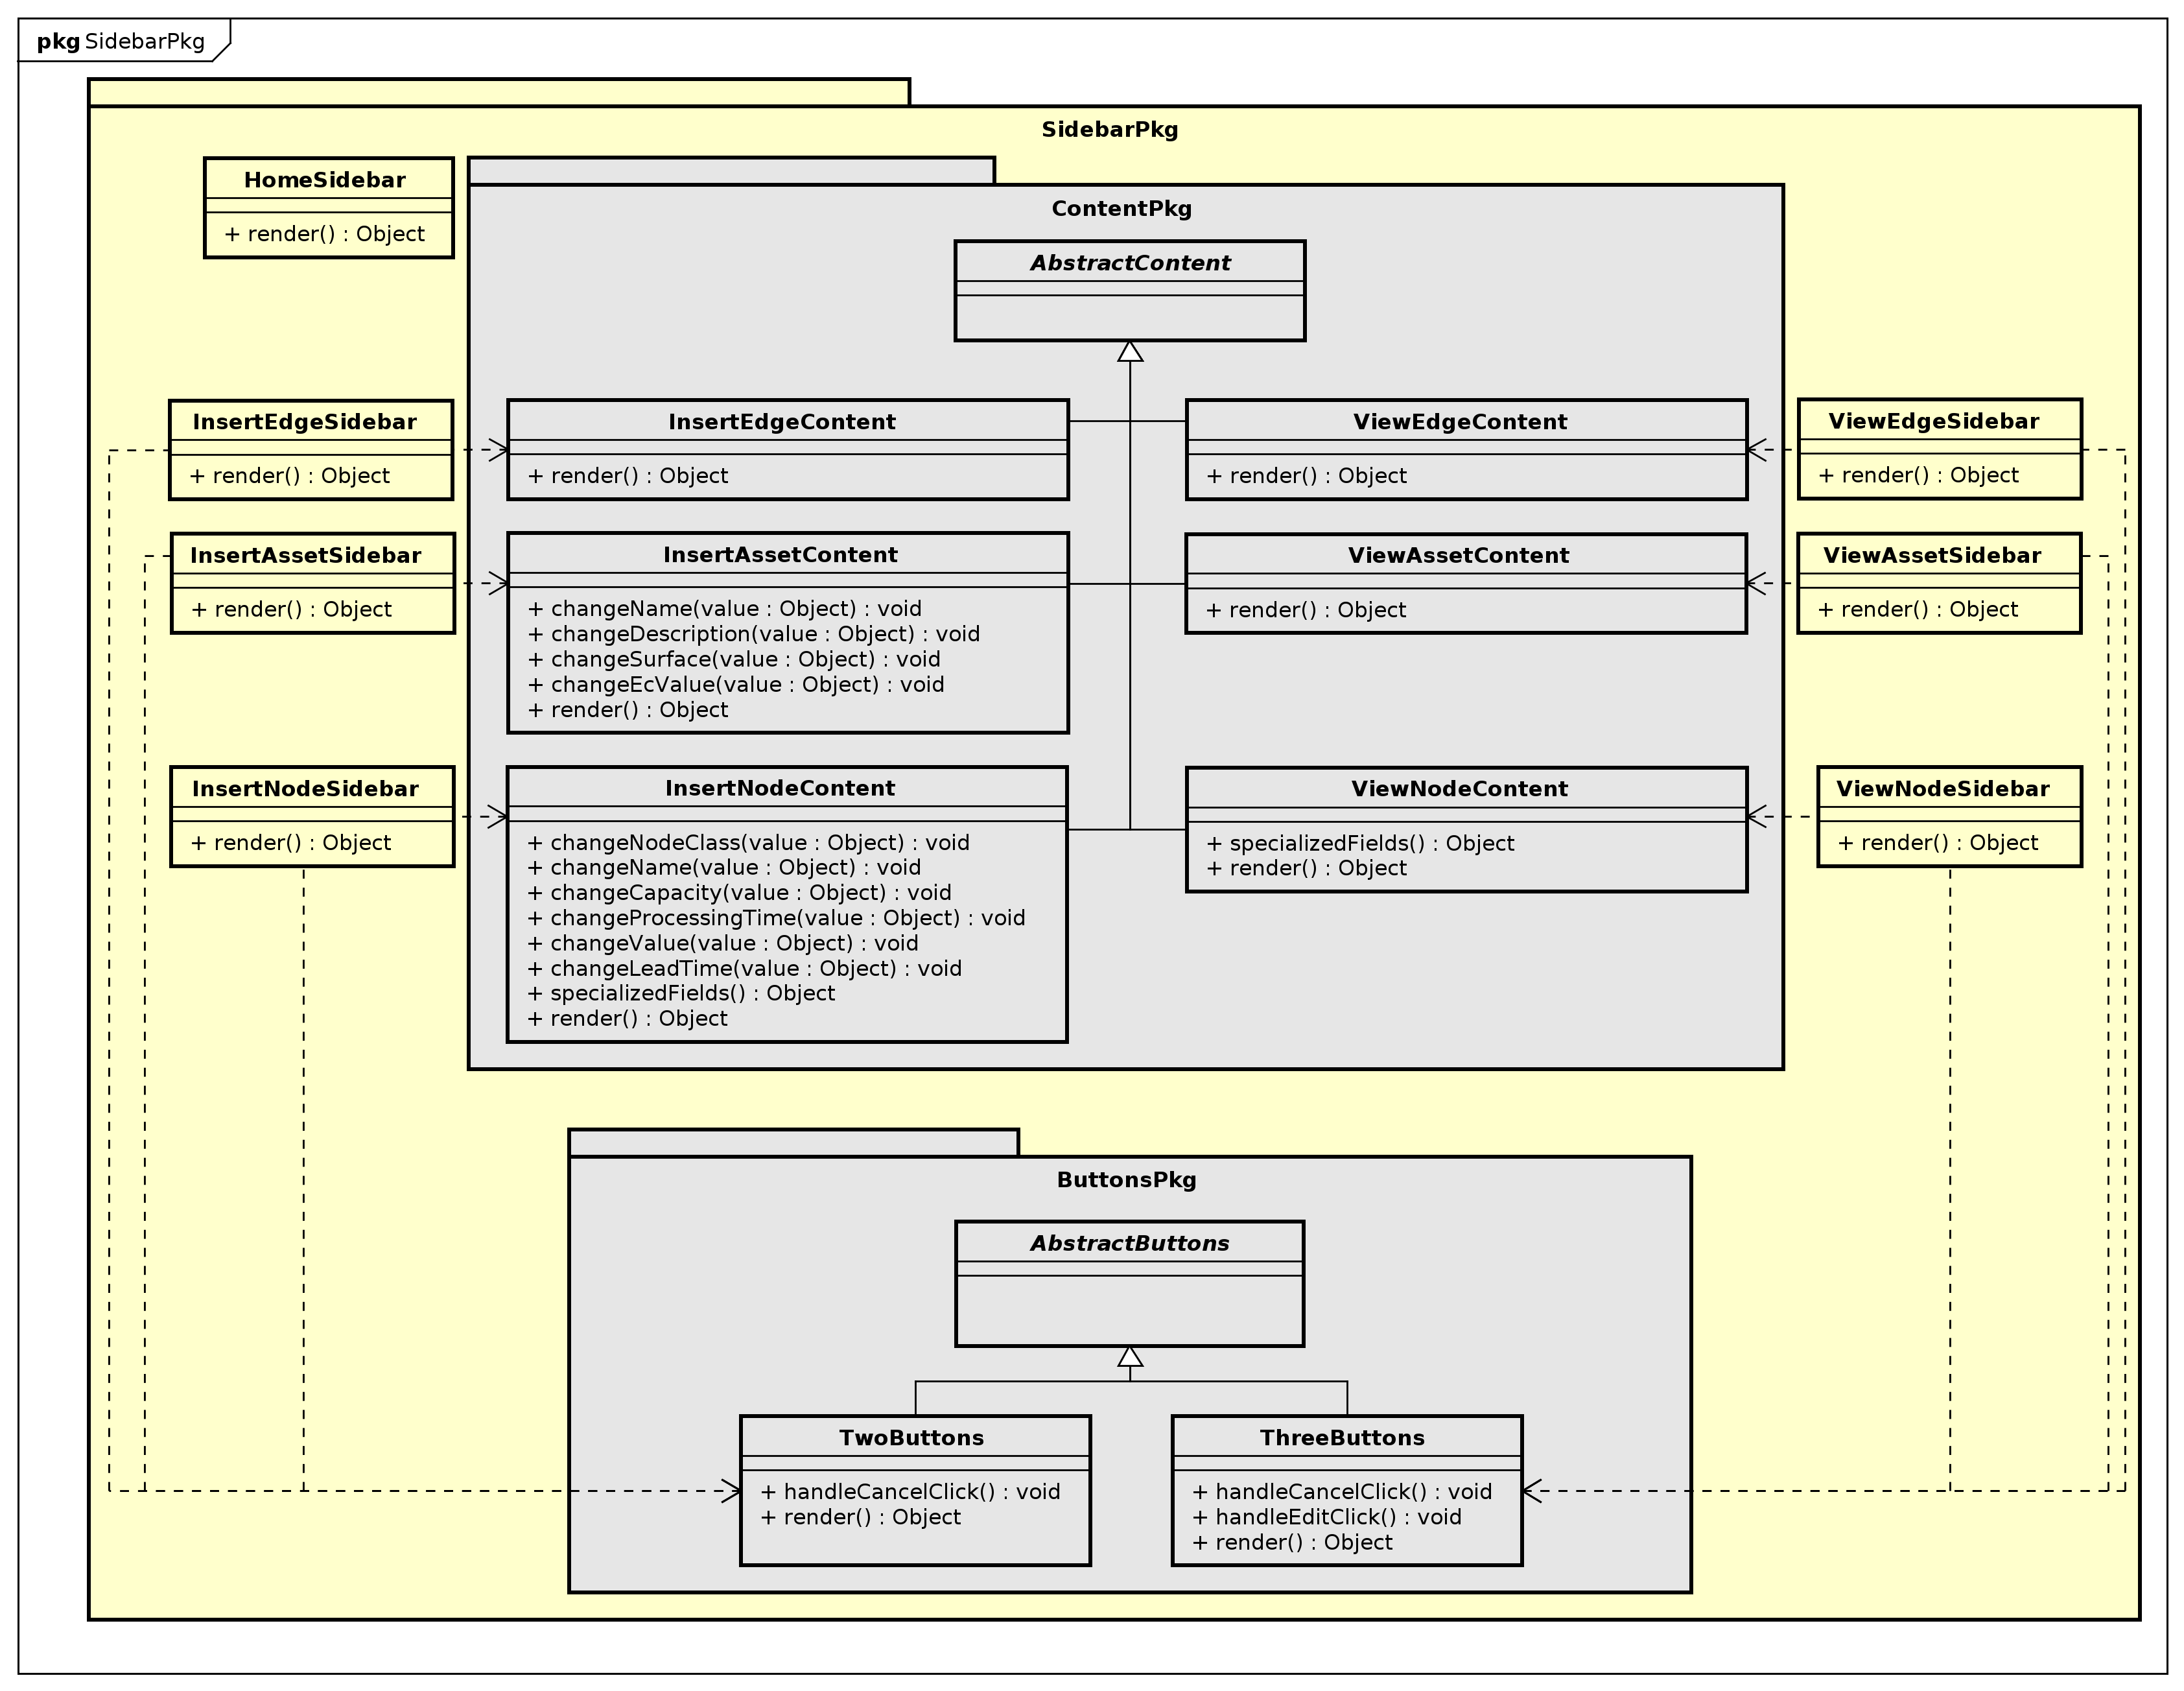
\includegraphics[width=\textwidth]{img/PkgDiagram/SidebarPkg.png}
	\caption{Schema componente DeGeOP::ViewPkg::SidebarPkg}
\end{figure}
\subsubsection{Informazioni sul package}
\begin{itemize}
	\item \textbf{descrizione:} racchiude le componenti necessarie alla rappresentazione della sidebar;
	\item \textbf{padre:} \hyperref[pkg::ViewPkg]{ViewPkg};
	\item \textbf{package contenuti:}
	\begin{itemize}
		\item SidebarPkg::\hyperref[pkg::ButtonsPkg]{ButtonsPkg};
		\item SidebarPkg::\hyperref[pkg::ContentPkg]{ContentPkg}.
	\end{itemize}
	\item \textbf{interazioni con altri package:} 
	\begin{itemize}
		\item IN DeGeOPViewPkg: utilizzo della sidebar.
	\end{itemize}
	\item \textbf{classi contenute:}
	\begin{itemize}
		\item HomeSidebar;
		\item InsertAssetSidebar;
		\item InsertEdgeSidebar;
		\item InsertNodeSidebar;
		\item ViewAssetSidebar;
		\item ViewEdgeSidebar;
		\item ViewNodeSidebar.
	\end{itemize}
\end{itemize}
\subsubsection{Classi}
\paragraph{HomeSidebar}
\begin{itemize}
	\begin{figure}[H]
		\centering
		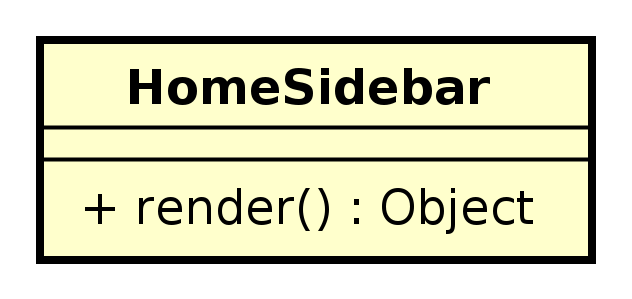
\includegraphics[width=0.3\textwidth]{./img/HomeSidebar.png}
		\caption{Diagramma classe HomeSidebar}
	\end{figure}
	\item \textbf{descrizione:} rappresenta la sidebar di default ;
	\item \textbf{utilizzo:} renderizza una sidebar di default che dà il benvenuto all'utente;
	\item \textbf{metodi:}
	\begin{itemize}
		\item +render() : Object\newline
		il metodo renderizza la sidebar di benvenuto
	\end{itemize}
\end{itemize}
\paragraph{InsertAssetSidebar}
\begin{itemize}
	\begin{figure}[H]
		\centering
		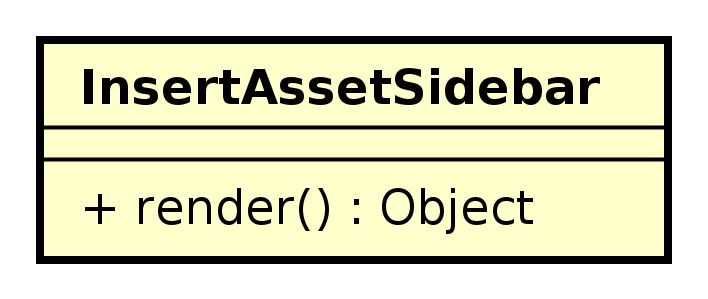
\includegraphics[width=0.3\textwidth]{./img/InsertAssetSidebar.png}
		\caption{Diagramma classe InsertAssetSidebar}
	\end{figure}
	\item \textbf{descrizione:} rappresenta una sidebar per l'inserimento e la modifica di un asset;
	\item \textbf{utilizzo:} renderizza una sidebar composta da contenuto in cui l'utente può compilare i dati e da bottoni che permettono di eseguire inserimenti e modifiche relative ad un asset;
	\item \textbf{metodi:}
	\begin{itemize}
		\item +render() : Object\newline
		il metodo renderizza la sidebar di inserimento e modifica di un asset, composta da un InsertAssetContent e da un TwoButtons
	\end{itemize}
\end{itemize}
\paragraph{InsertEdgeSidebar}
\begin{itemize}
	\begin{figure}[H]
		\centering
		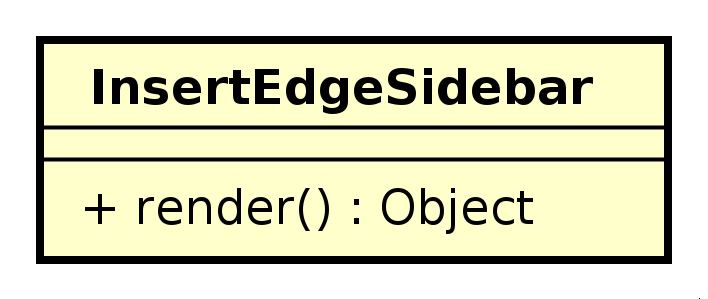
\includegraphics[width=0.3\textwidth]{./img/InsertEdgeSidebar.png}
		\caption{Diagramma classe InsertEdgeSidebar}
	\end{figure}
	\item \textbf{descrizione:} rappresenta una sidebar per l'inserimento e la modifica di un arco;
	\item \textbf{utilizzo:} renderizza una sidebar composta da contenuto in cui l'utente può compilare i dati e da bottoni che permettono di eseguire inserimenti e modifiche relative ad un arco;
	\item \textbf{metodi:}
	\begin{itemize}
		\item +render() : Object\newline
		il metodo renderizza la sidebar di inserimento e modifica di un arco, composta da un InsertEdgeContent e da un TwoButtons
	\end{itemize}
\end{itemize}
\paragraph{InsertNodeSidebar}
\begin{itemize}
	\begin{figure}[H]
		\centering
		\includegraphics[width=0.3\textwidth]{./img/InsertNodeSidebar.png}
		\caption{Diagramma classe InsertNodeSidebar}
	\end{figure}
	\item \textbf{descrizione:} rappresenta una sidebar per l'inserimento e la modifica di un nodo;
	\item \textbf{utilizzo:} renderizza una sidebar composta da contenuto in cui l'utente può compilare i dati e da bottoni che permettono di eseguire inserimenti e modifiche relative ad un nodo;
	\item \textbf{metodi:}
	\begin{itemize}
		\item +render() : Object\newline
		il metodo renderizza la sidebar di inserimento e modifica di un nodo, composta da un InsertNodeContent e da un TwoButtons
	\end{itemize}
\end{itemize}
\paragraph{ViewAssetSidebar}
\begin{itemize}
	\begin{figure}[H]
		\centering
		\includegraphics[width=0.3\textwidth]{./img/ViewAssetSidebar.png}
		\caption{Diagramma classe ViewAssetSidebar}
	\end{figure}
	\item \textbf{descrizione:} rappresenta una sidebar per la visualizzazione di un asset;
	\item \textbf{utilizzo:} renderizza una sidebar composta da contenuto in cui l'utente può visualizzare i dati e da bottoni che permettono di effettuare l'eliminazione dell'asset;
	\item \textbf{metodi:}
	\begin{itemize}
		\item +render() : Object\newline
		il metodo renderizza una sidebar per la visualizzazione di un asset, composta da un ViewAssetContent e da un ThreeButtons
	\end{itemize}
\end{itemize}
\paragraph{ViewEdgeSidebar}
\begin{itemize}
	\begin{figure}[H]
		\centering
		\includegraphics[width=0.3\textwidth]{./img/ViewEdgeSidebar.png}
		\caption{Diagramma classe ViewEdgeSidebar}
	\end{figure}
	\item \textbf{descrizione:} rappresenta una sidebar per l'inserimento e la modifica di un arco;
	\item \textbf{utilizzo:} renderizza una sidebar composta da contenuto in cui l'utente può visualizzare i dati e da bottoni che permettono di effettuare l'eliminazione dell'arco;
	\item \textbf{metodi:}
	\begin{itemize}
		\item +render() : Object\newline
		il metodo renderizza una sidebar per la visualizzazione di un arco, composta da un ViewEdgeContent e da un ThreeButtons
	\end{itemize}
\end{itemize}
\paragraph{ViewNodeSidebar}
\begin{itemize}
	\begin{figure}[H]
		\centering
		\includegraphics[width=0.3\textwidth]{./img/ViewNodeSidebar.png}
		\caption{Diagramma classe ViewNodeSidebar}
	\end{figure}
	\item \textbf{descrizione:} rappresenta una sidebar per la visualizzazione di un nodo;
	\item \textbf{utilizzo:} renderizza una sidebar composta da contenuto in cui l'utente può visualizzare i dati e da bottoni che permettono di effettuare l'eliminazione del nodo;
	\item \textbf{metodi:}
	\begin{itemize}
		\item +render() : Object\newline
		il metodo renderizza una sidebar per la visualizzazione di un arco, composta da un ViewNodeContent e da un ThreeButtons
	\end{itemize}
\end{itemize}
\newpage
\subsection{DeGeOP::ViewPkg::SidebarPkg::ContentPkg}
\label{pkg::ContentPkg}
\begin{figure}[H]
	\centering
	\includegraphics[width=\textwidth]{img/PkgDiagram/ContentPkg.png}
	\caption{Schema componente DeGeOP::ViewPkg::SidebarPkg::ContentPkg}
\end{figure}
\subsubsection{Informazioni sul package}
\begin{itemize}
	\item \textbf{descrizione:} racchiude le componenti che sono relative all'area informativa della Sidebar;
	\item \textbf{padre:} \hyperref[pkg::SidebarPkg]{SidebarPkg};
	\item \textbf{interazioni con altri package:} 
	\begin{itemize}
		\item IN FactorySidebarPkg: creazione contenuto della sidebar;
		\item OUT React-color: visualizzazione palette colori.
	\end{itemize}
	\item \textbf{classi contenute:}
	\begin{itemize}
		\item AbstractContent;
		\item InsertAssetContent;
		\item InsertEdgeContent;
		\item InsertNodeContent;
		\item ViewAssetContent;
		\item ViewEdgeContent;
		\item ViewNodeContent.
	\end{itemize}
\end{itemize}
\subsubsection{Classi}
\paragraph{AbstractContent}
\begin{itemize}
	\begin{figure}[H]
		\centering
		\includegraphics[width=0.3\textwidth]{./img/AbstractContent.png}
		\caption{Diagramma classe AbstractContent}
	\end{figure}
	\item \textbf{descrizione:} una classe d'interfaccia rappresentante il contenuto dell'area informativa nella sidebar;
	\item \textbf{utilizzo:} viene riferita da sidebar in quanto è una delle sue componenti.
\end{itemize}
\paragraph{InsertAssetContent}
\begin{itemize}
	\begin{figure}[H]
		\centering
		\includegraphics[width=0.3\textwidth]{./img/InsertAssetContent.png}
		\caption{Diagramma classe InsertAssetContent}
	\end{figure}
	\item \textbf{descrizione:} rappresenta il contenuto della sidebar relativa all'inserimento di un asset;
	\item \textbf{utilizzo:} viene creata da InsertAssetSidebarFactory ;
	\item \textbf{metodi:}
	\begin{itemize}
		\item +changeDescription() : void\newline
		delega il cambiamento dell'input della descrizione alla componente di livello più alto
		\item +changeEcValue(value) : void\newline
		delega il cambiamento dell'input del valore economico dell'asset alla componente di livello più alto
		\begin{itemize}
			\item value : string\\
			valore attualmente contenuto nell'input del valore economico dell'asset.
		\end{itemize}
		\item +changeName(value) : void\newline
		delega il cambiamento dell'input del nome dell'asset alla componente di livello più alto
		\begin{itemize}
			\item value : Object\\
			valore attualmente contenuto nell'input del nome dell'asset.
		\end{itemize}
		\item +changeSurface() : void\newline
		delega il cambiamento dell'input della superficie dell'asset alla componente di livello più alto
		\item +render() : Object\newline
		renderizza il contenuto della sidebar dell'asset in modalità inserimento e modifica
	\end{itemize}
\end{itemize}
\paragraph{InsertEdgeContent}
\begin{itemize}
	\begin{figure}[H]
		\centering
		\includegraphics[width=0.3\textwidth]{./img/InsertEdgeContent.png}
		\caption{Diagramma classe InsertEdgeContent}
	\end{figure}
	\item \textbf{descrizione:} rappresenta il contenuto della sidebar relativa all'inserimento di un arco;
	\item \textbf{utilizzo:} viene creata da InsertEdgeSidebarFactory ;
	\item \textbf{metodi:}
	\begin{itemize}
		\item +render() : Object\newline
		renderizza il contenuto della sidebar dell'arco in modalità inserimento e modifica
	\end{itemize}
\end{itemize}
\paragraph{InsertNodeContent}
\begin{itemize}
	\begin{figure}[H]
		\centering
		\includegraphics[width=0.3\textwidth]{./img/InsertNodeContent.png}
		\caption{Diagramma classe InsertNodeContent}
	\end{figure}
	\item \textbf{descrizione:} rappresenta il contenuto della sidebar relativa all'inserimento di un nodo;
	\item \textbf{utilizzo:} viene creata da InsertNodeSidebarFactory ;
	\item \textbf{metodi:}
	\begin{itemize}
		\item +changeCapacity() : void\newline
		delega il cambiamento della capacità del nodo alla componente di più alto livello
		\item +changeLeadTime(value) : void\newline
		delega il cambiamento del tempo di approvigionamento del nodo alla componente di più alto livello
		\begin{itemize}
			\item value : string\\
			valore che è contenuto nel dropdown della classe del nodo.
		\end{itemize}
		\item +changeName(value) : void\newline
		delega il cambiamento del nome del nodo alla componente di più alto livello
		\begin{itemize}
			\item value : string\\
			valore che è contenuto nel dropdown della classe del nodo.
		\end{itemize}
		\item +changeNodeClass(value) : void\newline
		delega il cambiamento del dropdown del nome del nodo alla componente di più alto livello
		\begin{itemize}
			\item value : string\\
			valore che è contenuto nel dropdown della classe del node.
		\end{itemize}
		\item +changeProcessingTime(value) : void\newline
		delega il cambiamento del valore del nodo alla componente di più alto livello
		\begin{itemize}
			\item value : string\\
			valore che è contenuto nel dropdown della classe del nodo.
		\end{itemize}
		\item +render() : Object\newline
		renderizza il il contenuto della sidebar del node in modalità inserimento e modifica
		\item +specializedFields() : Object\newline
		metodo che gestisce i campi dati da visualizzare a seconda della tipologia del nodo
	\end{itemize}
\end{itemize}
\paragraph{ViewAssetContent}
\begin{itemize}
	\begin{figure}[H]
		\centering
		\includegraphics[width=0.3\textwidth]{./img/ViewAssetContent.png}
		\caption{Diagramma classe ViewAssetContent}
	\end{figure}
	\item \textbf{descrizione:} rappresenta il contenuto della sidebar relativa alla visualizzazione di un asset;
	\item \textbf{utilizzo:} viene creata da ViewAssetSidebarFactory ;
	\item \textbf{metodi:}
	\begin{itemize}
		\item +render() : Object\newline
		renderizza la parte di sidebar relativa alla visualizzazione dei campi dati di un asset
	\end{itemize}
\end{itemize}
\paragraph{ViewEdgeContent}
\begin{itemize}
	\begin{figure}[H]
		\centering
		\includegraphics[width=0.3\textwidth]{./img/ViewEdgeContent.png}
		\caption{Diagramma classe ViewEdgeContent}
	\end{figure}
	\item \textbf{descrizione:} rappresenta il contenuto della sidebar relativa alla visualizzazione di un arco;
	\item \textbf{utilizzo:} viene creata da ViewEdgeSidebarFactory ;
	\item \textbf{metodi:}
	\begin{itemize}
		\item +render() : Object\newline
		renderizza la parte di sidebar relativa alla visualizzazione dei campi dati di un arco
		\item +specializedFields() : Object\newline
		si occupa della visualizzazione dei campi dati a seconda della tipologia del nodo
	\end{itemize}
\end{itemize}
\paragraph{ViewNodeContent}
\begin{itemize}
	\begin{figure}[H]
		\centering
		\includegraphics[width=0.3\textwidth]{./img/ViewNodeContent.png}
		\caption{Diagramma classe ViewNodeContent}
	\end{figure}
	\item \textbf{descrizione:} rappresenta il contenuto della sidebar relativa alla visualizzazione di un ndo;
	\item \textbf{utilizzo:} viene creata da ViewNodeSidebarFactory ;
	\item \textbf{metodi:}
	\begin{itemize}
		\item +render() : Object\newline
		renderizza la parte di sidebar relativa alla visualizzazione dei campi dati di un nodo
	\end{itemize}
\end{itemize}
\newpage
\subsection{DeGeOP::ViewPkg::SidebarPkg::ButtonsPkg}
\label{pkg::ButtonsPkg}
\begin{figure}[H]
	\centering
	\includegraphics[width=\textwidth]{img/PkgDiagram/ButtonsPkg.png}
	\caption{Schema componente DeGeOP::ViewPkg::SidebarPkg::ButtonsPkg}
\end{figure}
\subsubsection{Informazioni sul package}
\begin{itemize}
	\item \textbf{descrizione:} racchiude le componenti che sono relative all'area con i bottoni della Sidebar;
	\item \textbf{padre:} \hyperref[pkg::SidebarPkg]{SidebarPkg};
	\item \textbf{classi contenute:}
	\begin{itemize}
		\item AbstractButtons;
		\item ThreeButtons;
		\item TwoButtons.
	\end{itemize}
\end{itemize}
\subsubsection{Classi}
\paragraph{AbstractButtons}
\begin{itemize}
	\begin{figure}[H]
		\centering
		\includegraphics[width=0.3\textwidth]{./img/AbstractButtons.png}
		\caption{Diagramma classe AbstractButtons}
	\end{figure}
	\item \textbf{descrizione:} una classe d'interfaccia rappresentante i bottoni inseriti nella sidebar;
	\item \textbf{utilizzo:} viene riferita da sidebar in quanto è una delle sue componenti.
\end{itemize}
\paragraph{ThreeButtons}
\begin{itemize}
	\begin{figure}[H]
		\centering
		\includegraphics[width=0.3\textwidth]{./img/ThreeButtons.png}
		\caption{Diagramma classe ThreeButtons}
	\end{figure}
	\item \textbf{descrizione:} classe che renderizza tre bottoni, uno di modifica,  uno di eliminazione e uno di annullamento. Il bottone di annullamento provoca l'annullamento della selezione corrente. Il bottone di eliminazione provoca la comparsa di una finestra modale che chiede la conferma dell'eliminazione dell'elemento correntemente selezionato. Il bottone di modifica provoca l'avvio della modalità di modifica, con cui è possibile ridisegnare l'asset o cambiare i campi dati;
	\item \textbf{utilizzo:} viene utilizzata nelle sidebar di visualizzazione;
	\item \textbf{metodi:}
	\begin{itemize}
		\item +handleCancelClick() : void\newline
		il metodo gestisce il click sul bottone di annullamento, ripristinando la sidebar di default
		\item +handleEditClick() : void\newline
		il metodo imposta la sidebar di modifica dell'elemento attualmente selezionato
		\item +render() : Object\newline
		renderizza tre bottoni, uno di modifica, uno di annullamento e uno di eliminazione
	\end{itemize}
\end{itemize}
\paragraph{TwoButtons}
\begin{itemize}
	\begin{figure}[H]
		\centering
		\includegraphics[width=0.3\textwidth]{./img/TwoButtons.png}
		\caption{Diagramma classe TwoButtons}
	\end{figure}
	\item \textbf{descrizione:} classe che renderizza due bottoni, uno di salvataggio e uno di annullamento. Il bottone di salvataggio è disabilitato fino a che tutti i campi della sidebar non sono stati compilati in modo corretto. Il bottone di annullamento provoca l'interruzione dell'inserimento dei dati;
	\item \textbf{utilizzo:} viene utilizzata nelle sidebar di inserimento;
	\item \textbf{metodi:}
	\begin{itemize}
		\item +handleCancelClick() : void\newline
		il metodo gestisce il click sul bottone di annullamento, ripristinando la sidebar di default
		\item +render() : Object\newline
		renderizza due bottoni, uno di annullamento e uno di salvataggio
	\end{itemize}
\end{itemize}
\newpage
